%% The "\appendix" call has already been made in the declaration
%% of the "appendices" environment (see thesis.tex).
\chapter{Appendix: Search strategy}
\label{app:analysis}

%\chapterquote{%
%Le savant n'\'etudie pas la nature parce que cela est utile; \\
%\indent il l'\'etudie parce qu'il y prend plaisir, \\
%\indent et il y prend plaisir parce qu'elle est belle.}%
%{Henri Poincar\'e, 1854--1912}

%Appendixes (or should that be ``appendices''?) make you look really clever, 
%%%'cos it's like you had more clever stuff to say than could be fitted into 
%%%the %%%%main bit of your thesis. Yeah. So everyone should have at least 
%%%%%%%three of %%%%%them\dots

%% Big appendixes should be split off into separate files, just like chapters
%\input{app-myreallybigappendix}

%Data/MC plots or 
%plots showing the contributions of different backgrounds in 
%the SR/CRs. And/or yields (section 4 in AN).

\section{Uncertainties on transfer factors derived from variations in 
simulation}
\label{app:tfvariations}
This appendix shows the changes of the transfer factors, which are used to 
assign systematic uncertainties to them, upon varying the various correction 
factors applied to the simulation (Sec.~\ref{sec:analysis-mccorrections}) by 
one standard deviation up and down according to their measured uncertainties. 
This is discussed in Sec.~\ref{sec:analysis-systematics-mc}.

\begin{figure}[h!]
	\subfloat{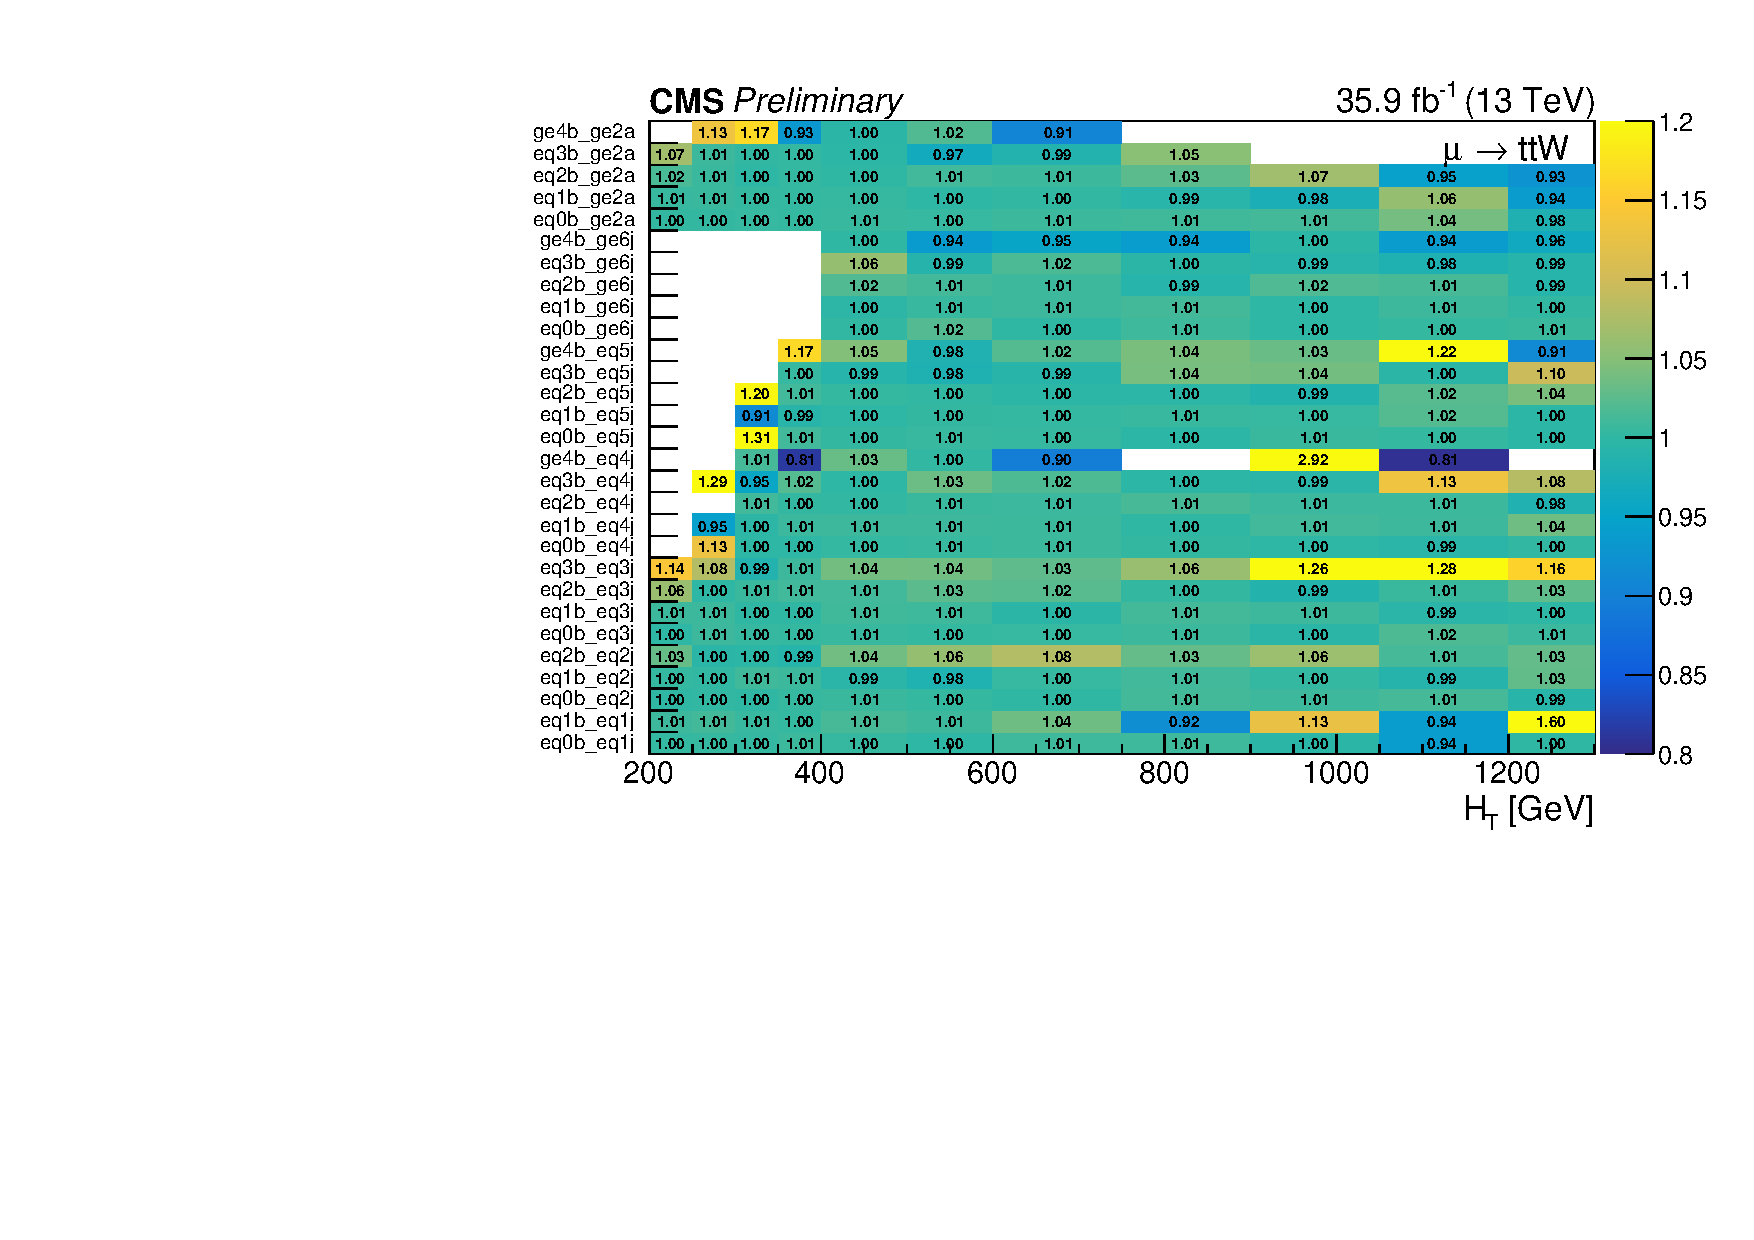
\includegraphics[width=0.5\textwidth]{figs/analysis/transferfactors/tfratio_mu_Ttw_2d_puWeightUp}}~
	\subfloat{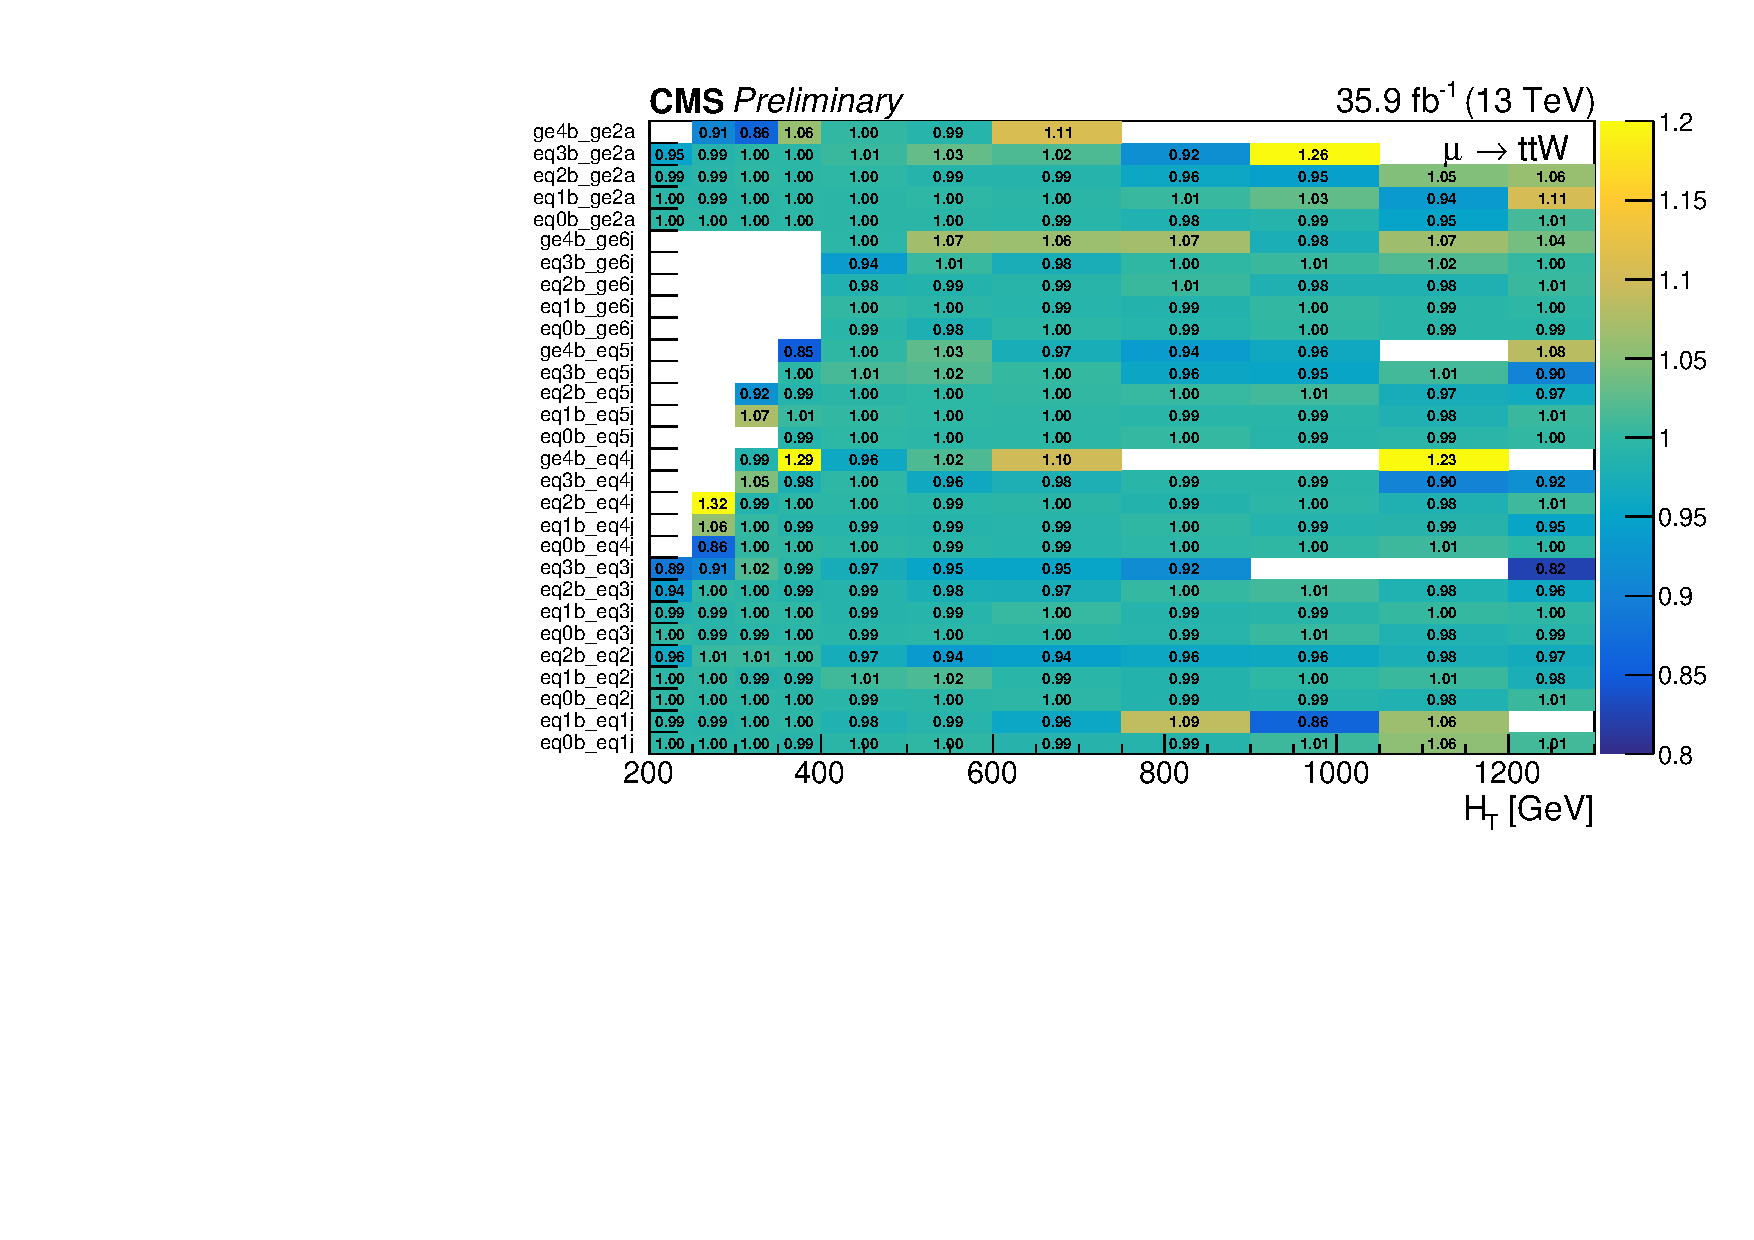
\includegraphics[width=0.5\textwidth]{figs/analysis/transferfactors/tfratio_mu_Ttw_2d_puWeightDown}}\\
	\subfloat{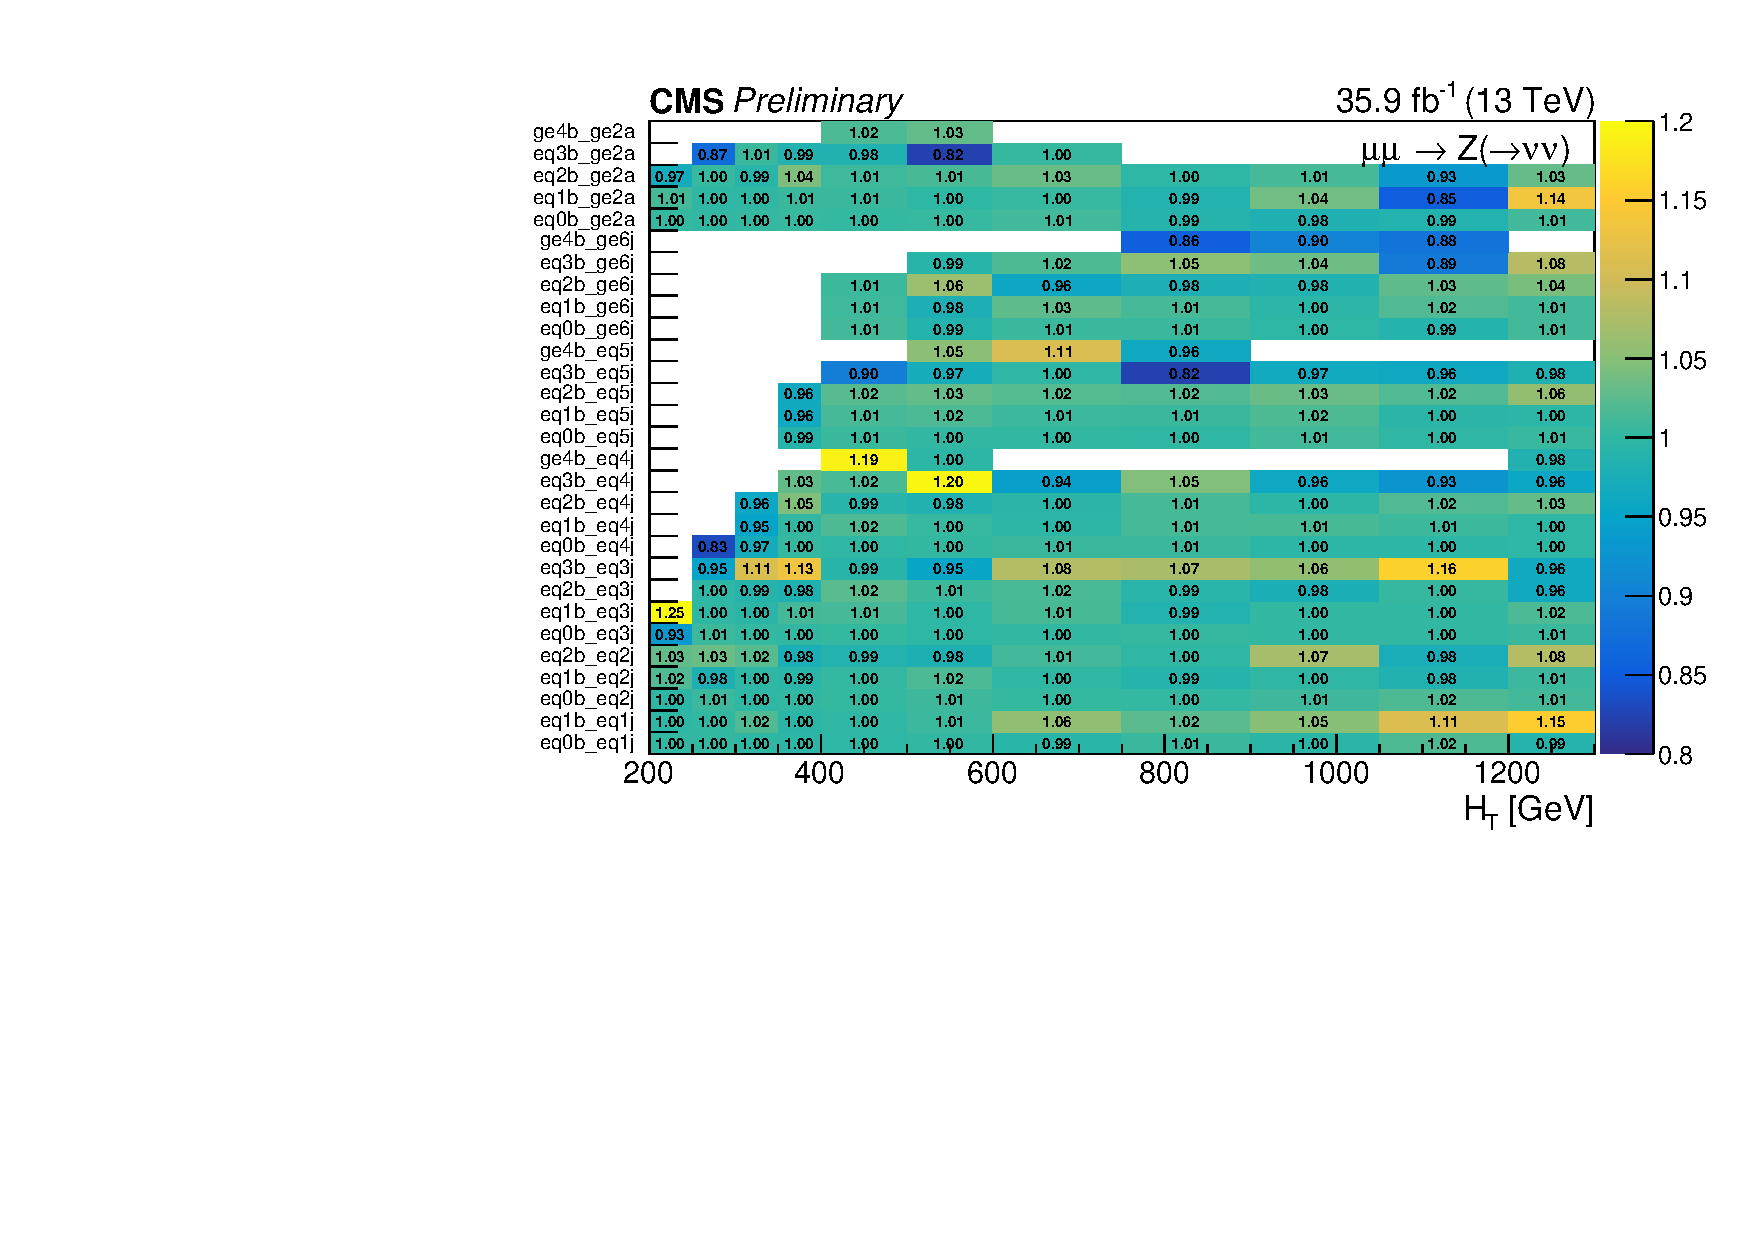
\includegraphics[width=0.5\textwidth]{figs/analysis/transferfactors/tfratio_mumu_Zinv_2d_puWeightUp}}~
	\subfloat{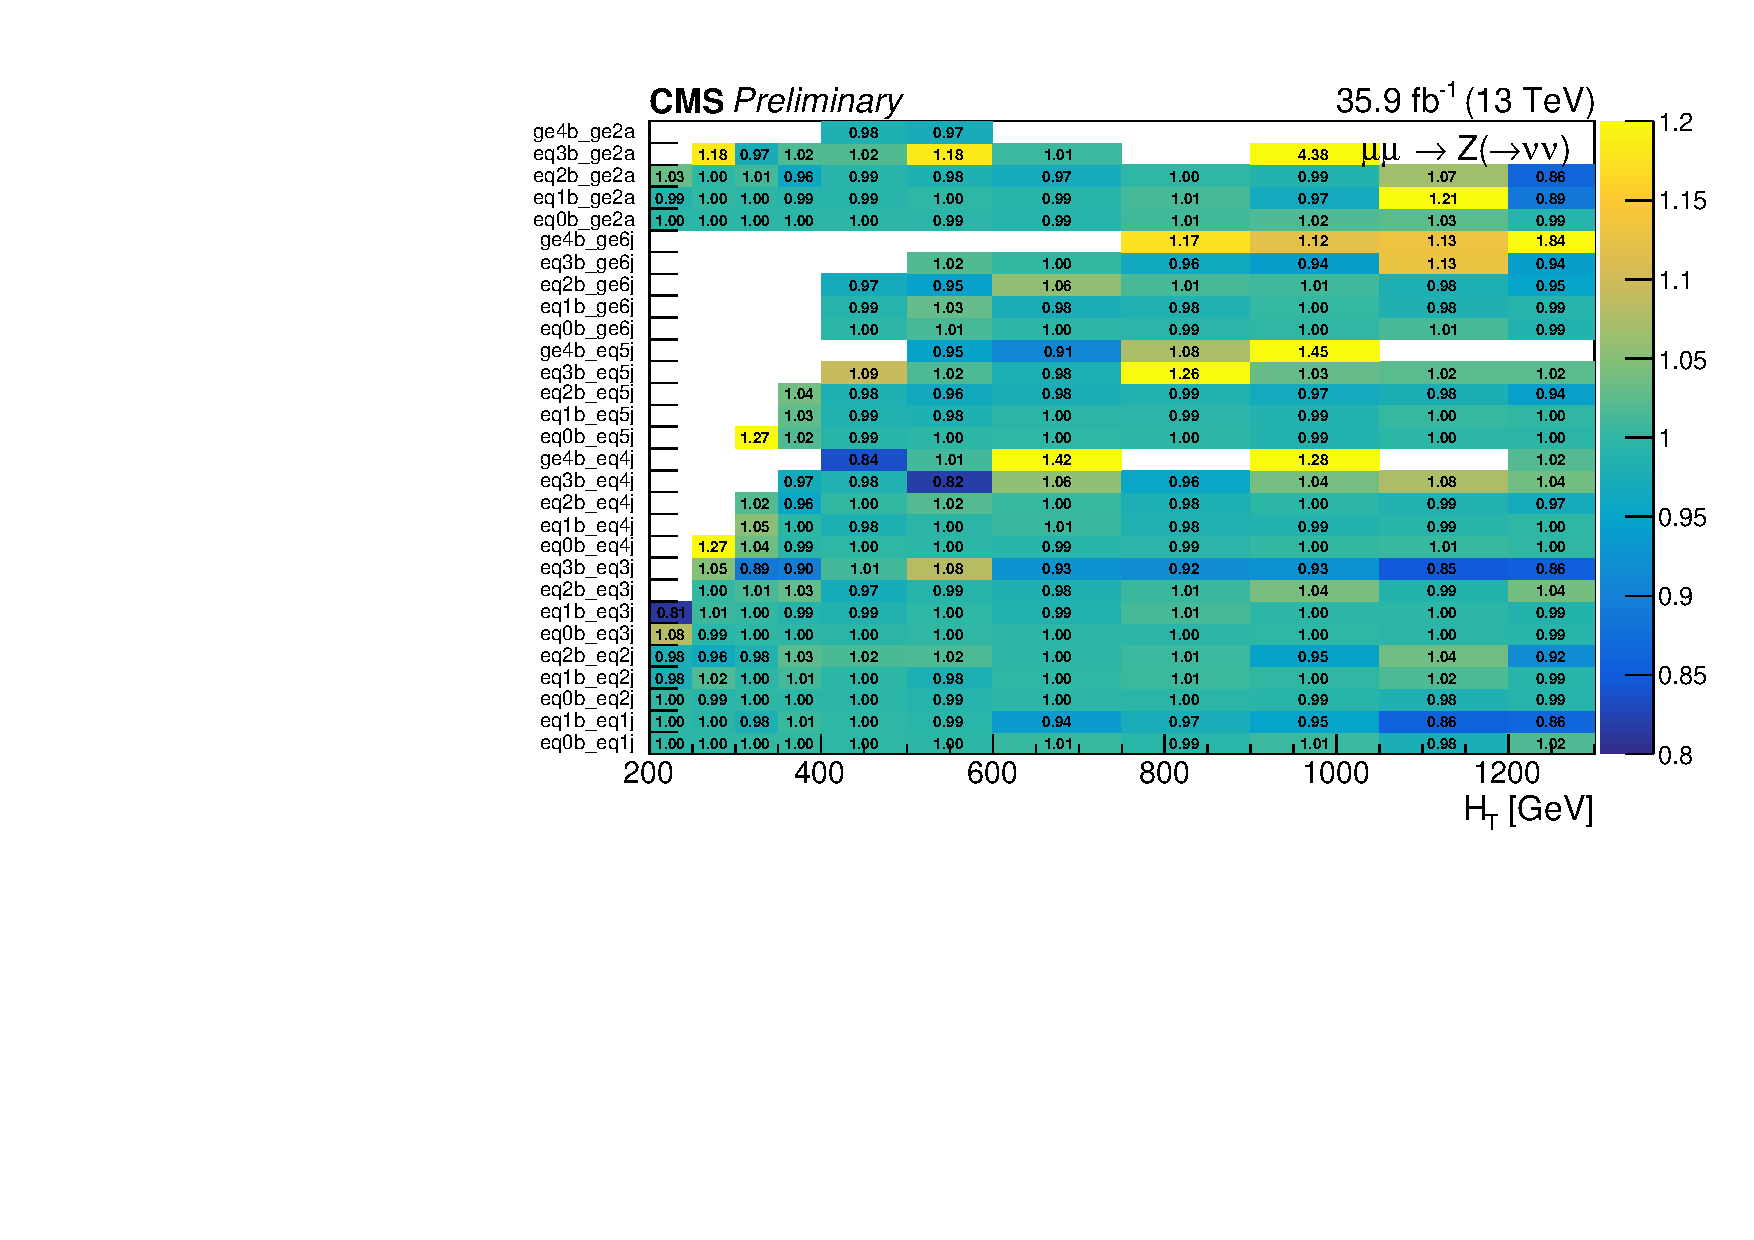
\includegraphics[width=0.5\textwidth]{figs/analysis/transferfactors/tfratio_mumu_Zinv_2d_puWeightDown}}\\
	\caption{The ratio of the \Tmutottw (top) and \Tmumutoz (bottom) transfer 
		factors in each \njnbht bin when varying the pileup correction factors 
		by $+1\sigma$ (left) and $-1\sigma$ (right) with respect to 
		their nominal values.}
	\label{fig:tfvariations-pileup}
\end{figure}

\begin{figure}[h!]
	\subfloat{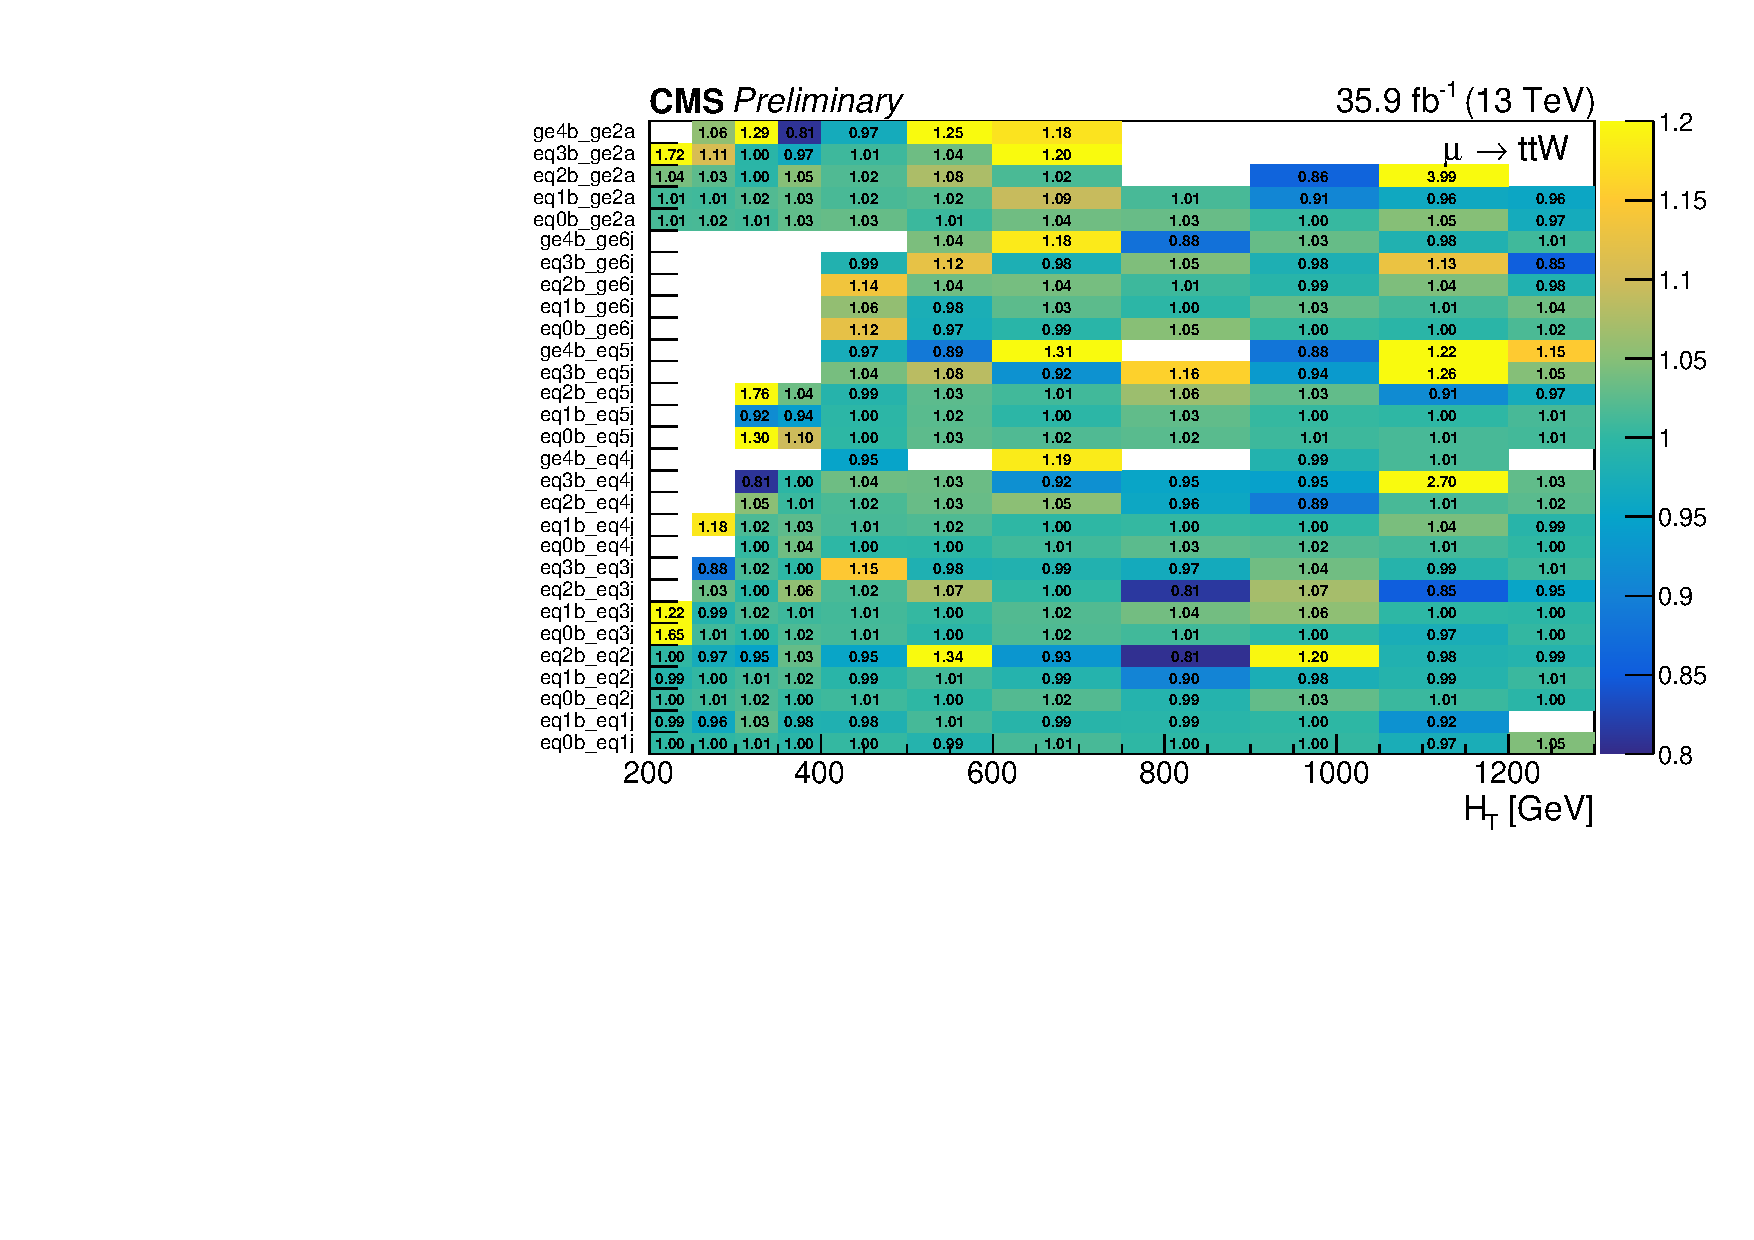
\includegraphics[width=0.5\textwidth]{figs/analysis/transferfactors/tfratio_mu_Ttw_2d_jecUp}}~
	\subfloat{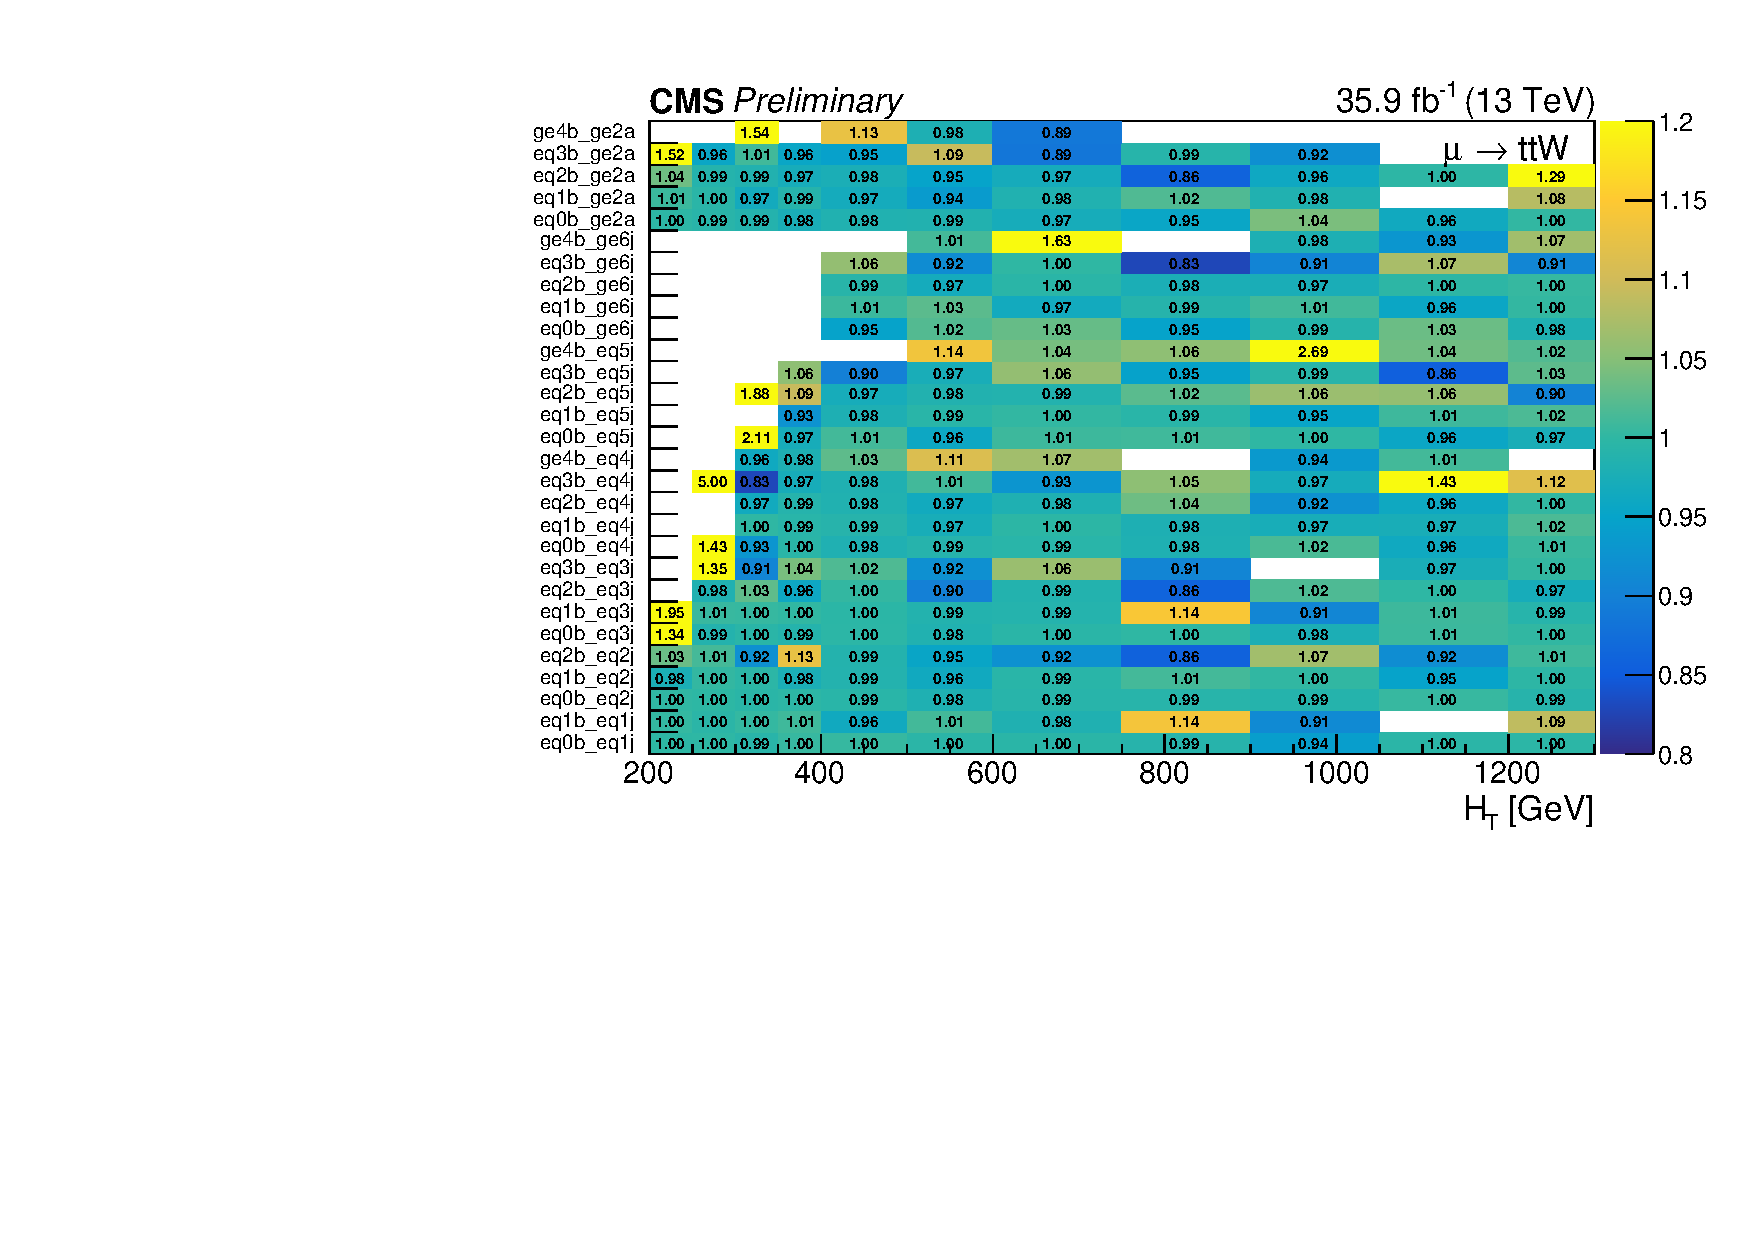
\includegraphics[width=0.5\textwidth]{figs/analysis/transferfactors/tfratio_mu_Ttw_2d_jecDown}}\\
	\subfloat{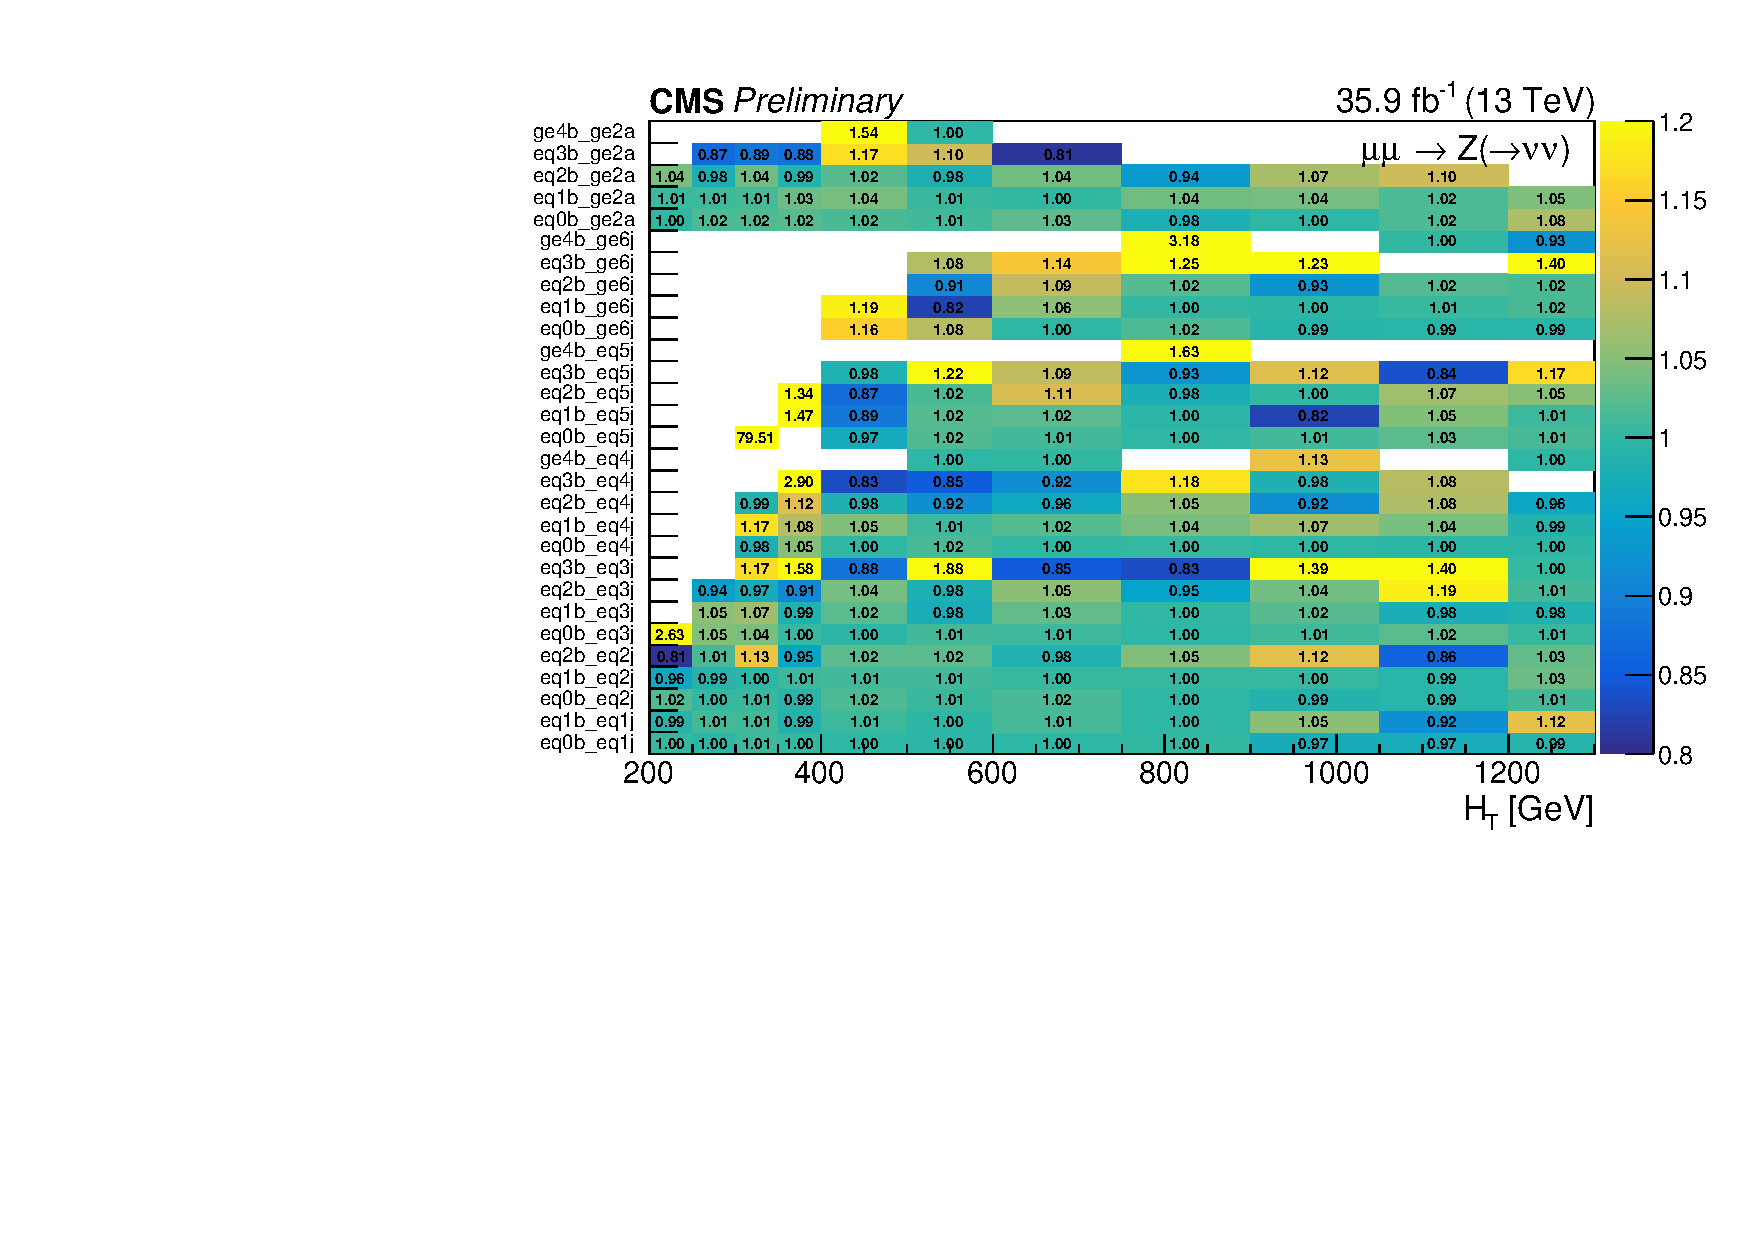
\includegraphics[width=0.5\textwidth]{figs/analysis/transferfactors/tfratio_mumu_Zinv_2d_jecUp}}~
	\subfloat{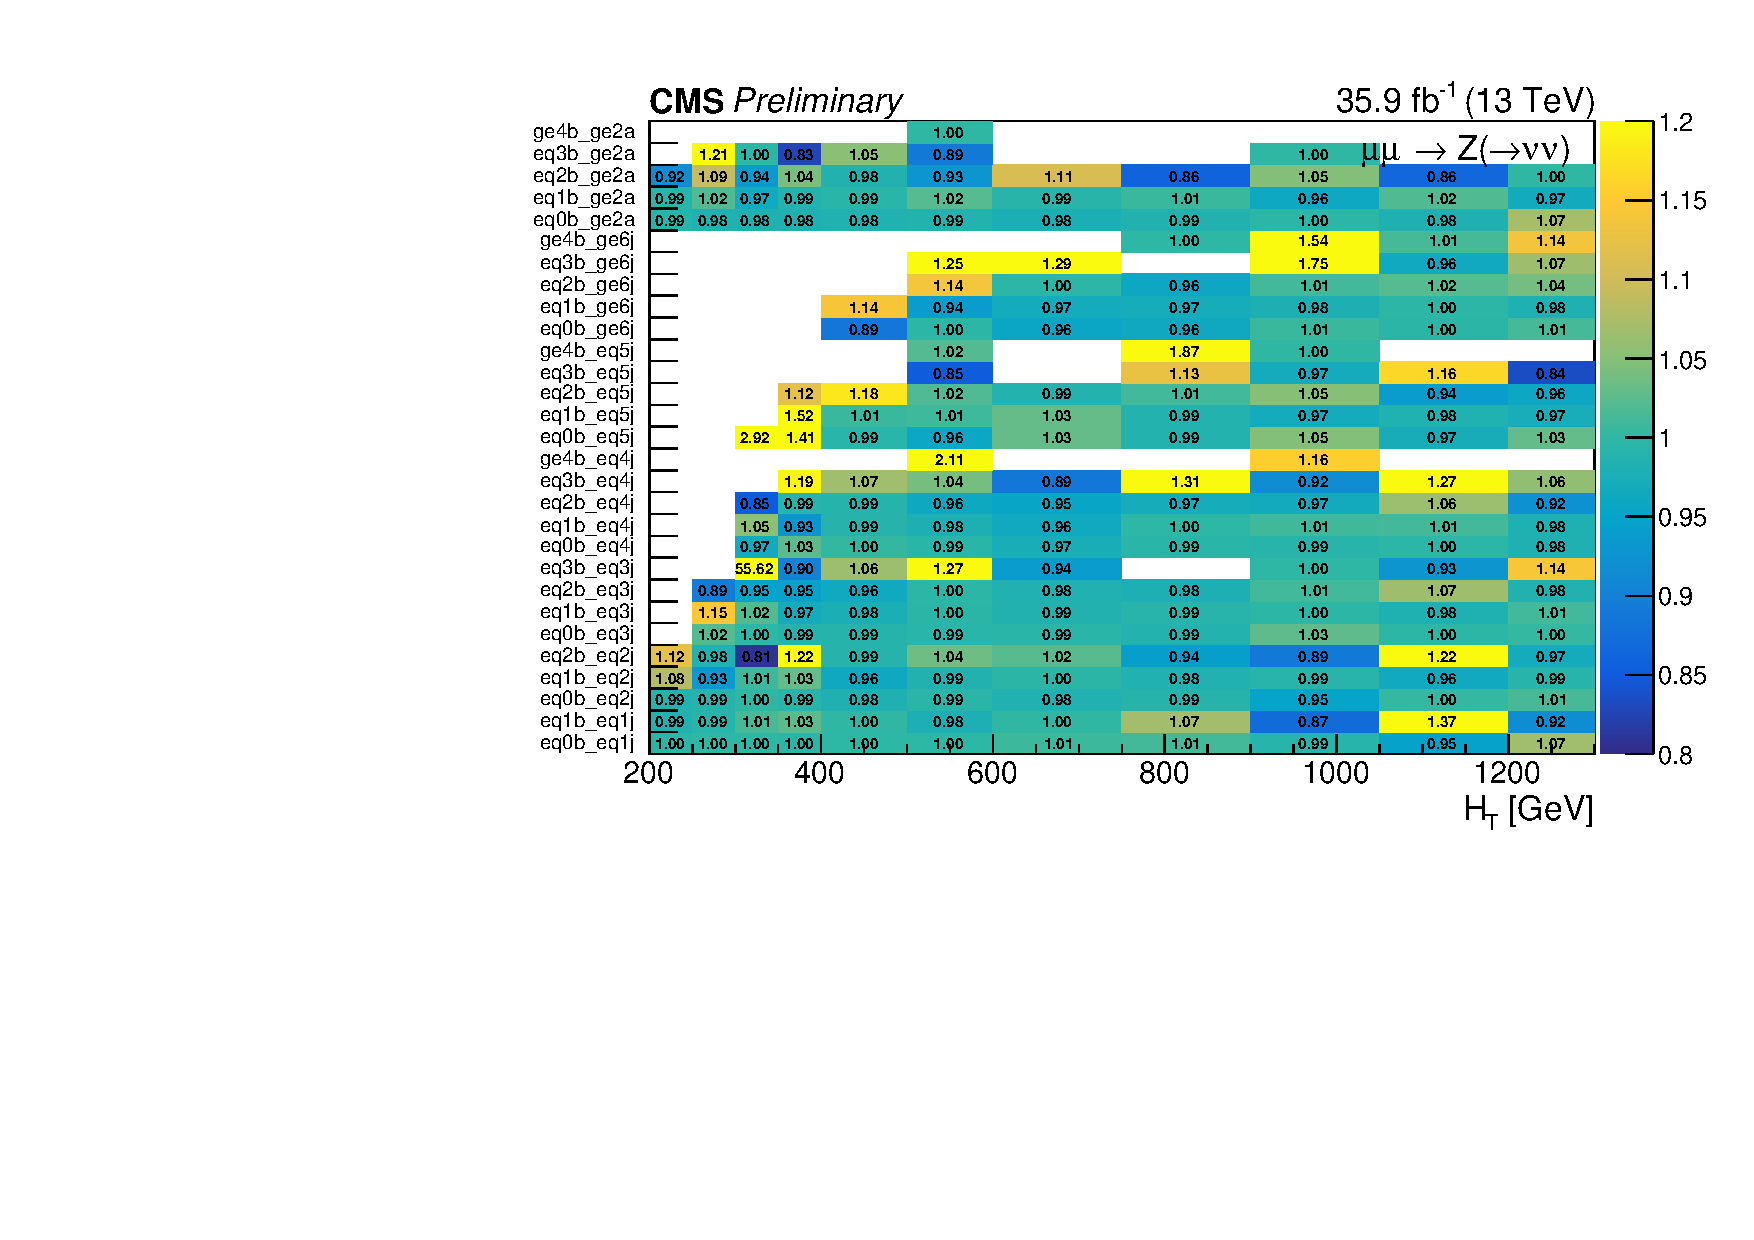
\includegraphics[width=0.5\textwidth]{figs/analysis/transferfactors/tfratio_mumu_Zinv_2d_jecDown}}\\
	\caption{The ratio of the \Tmutottw (top) and \Tmumutoz (bottom) transfer 
		factors in each \njnbht bin when varying the jet energy correction 
		factors by $+1\sigma$ (left) and $-1\sigma$ (right) with respect to 
		their nominal values.}
	\label{fig:tfvariations-jec}
\end{figure}

\begin{figure}[h!]
	\subfloat{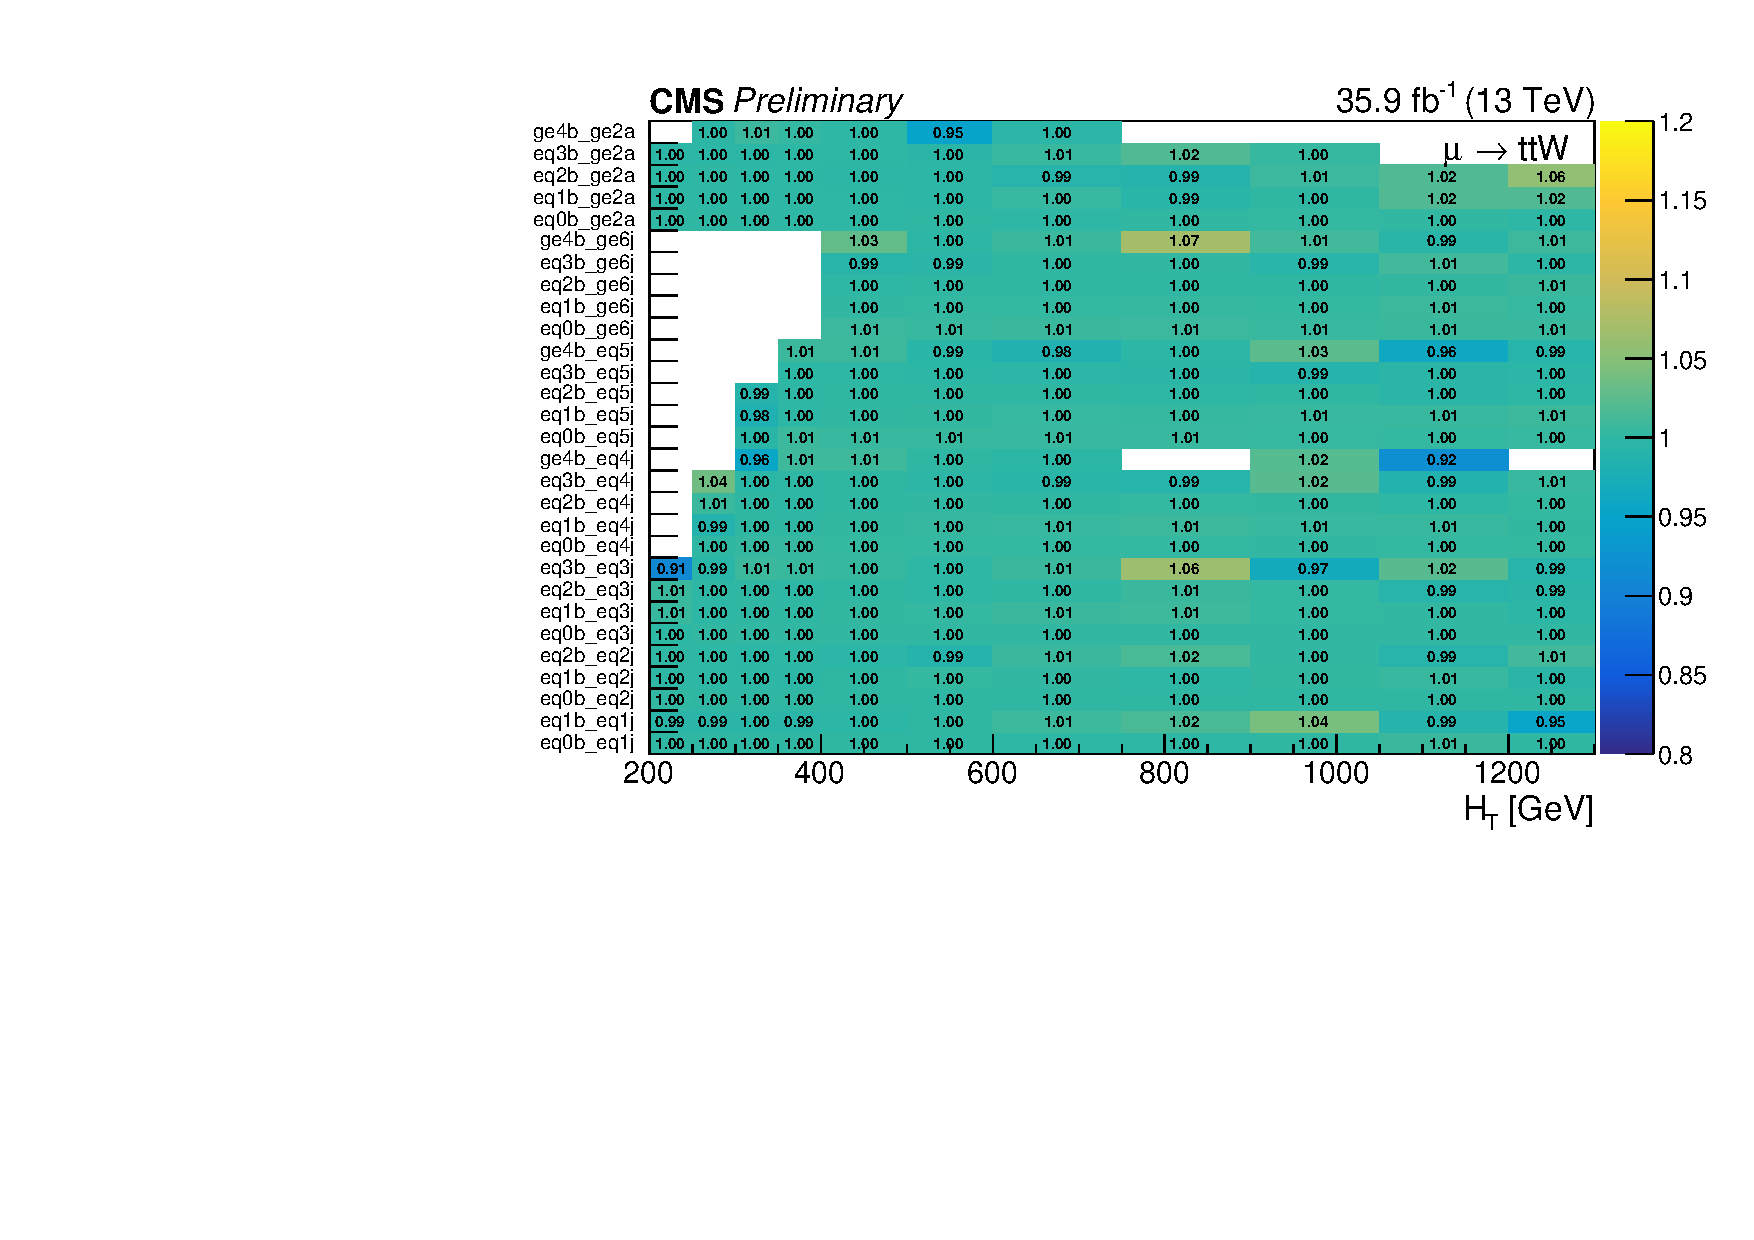
\includegraphics[width=0.5\textwidth]{figs/analysis/transferfactors/tfratio_mu_Ttw_2d_bsfWeightUp}}~
	\subfloat{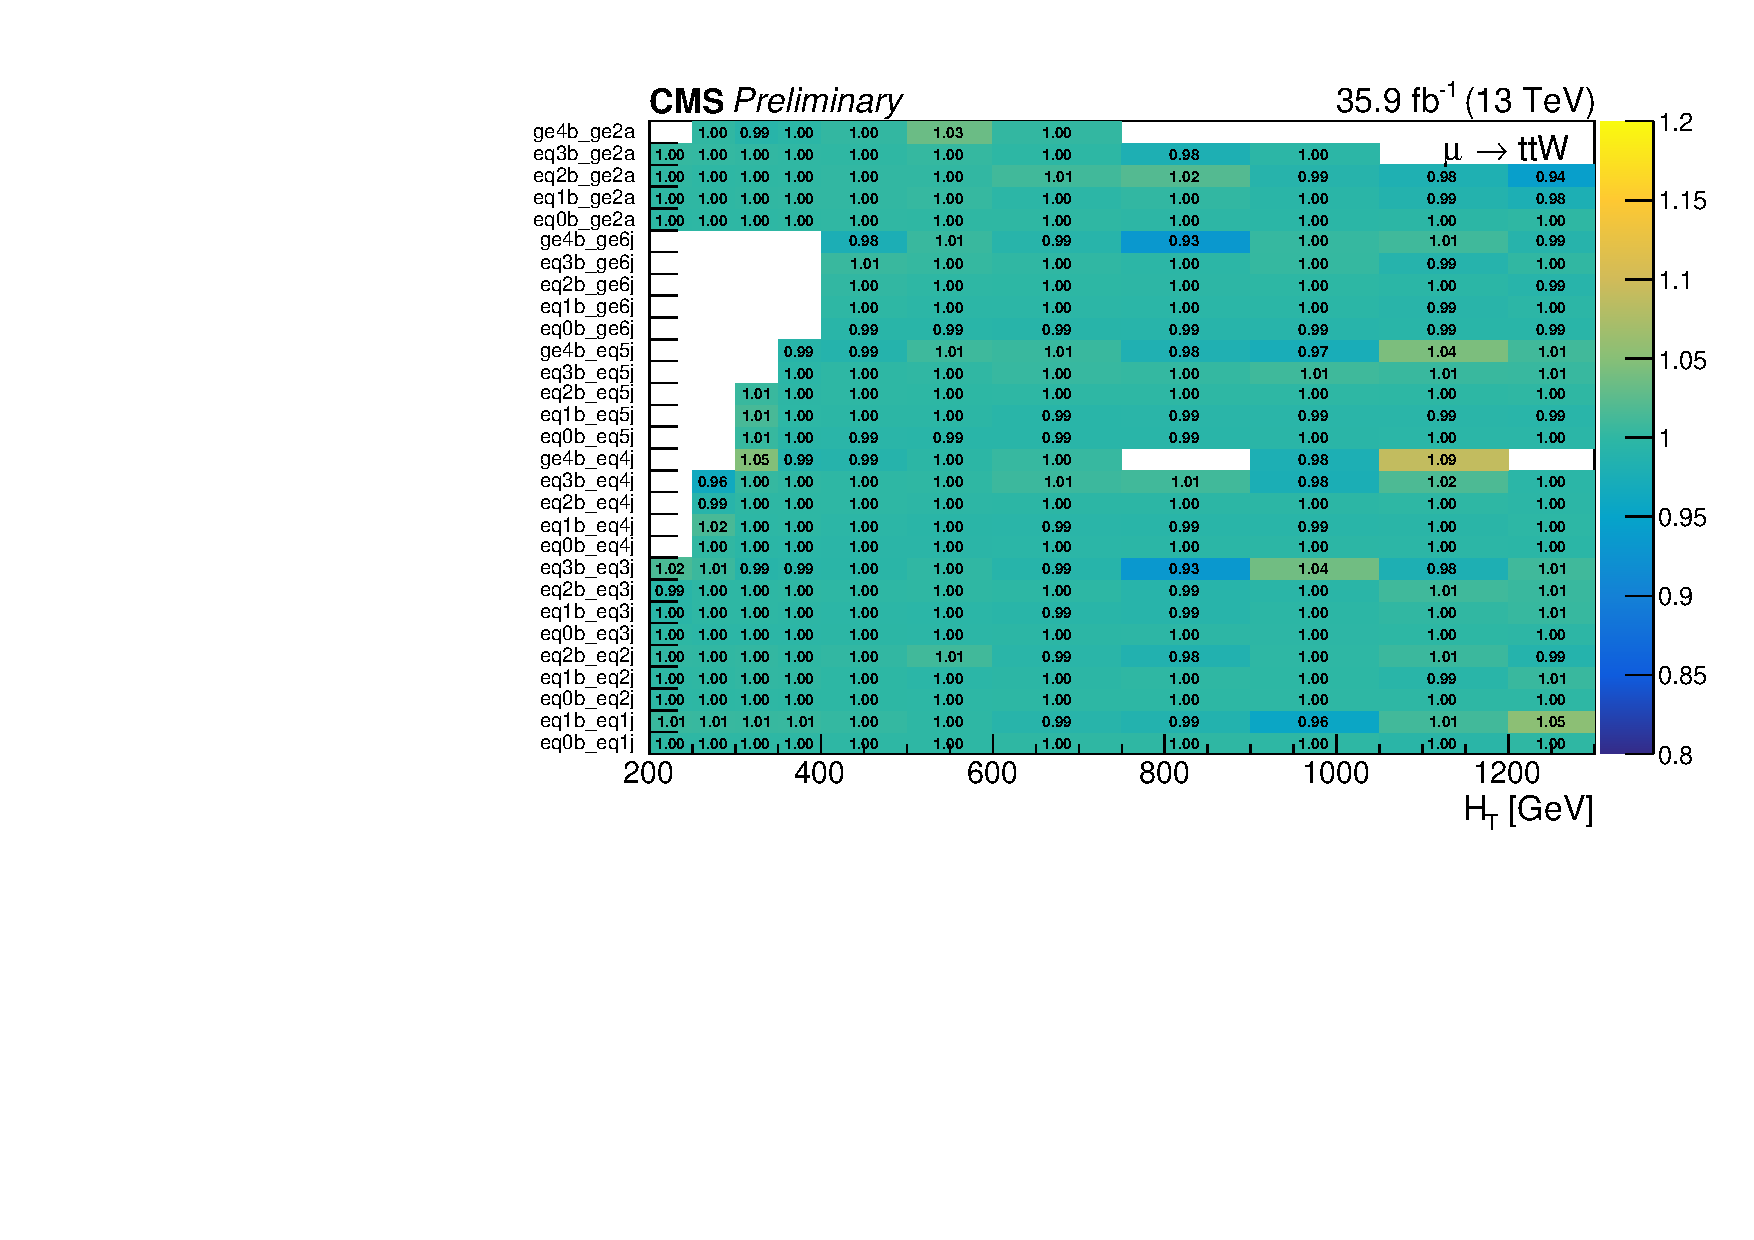
\includegraphics[width=0.5\textwidth]{figs/analysis/transferfactors/tfratio_mu_Ttw_2d_bsfWeightDown}}\\
	\subfloat{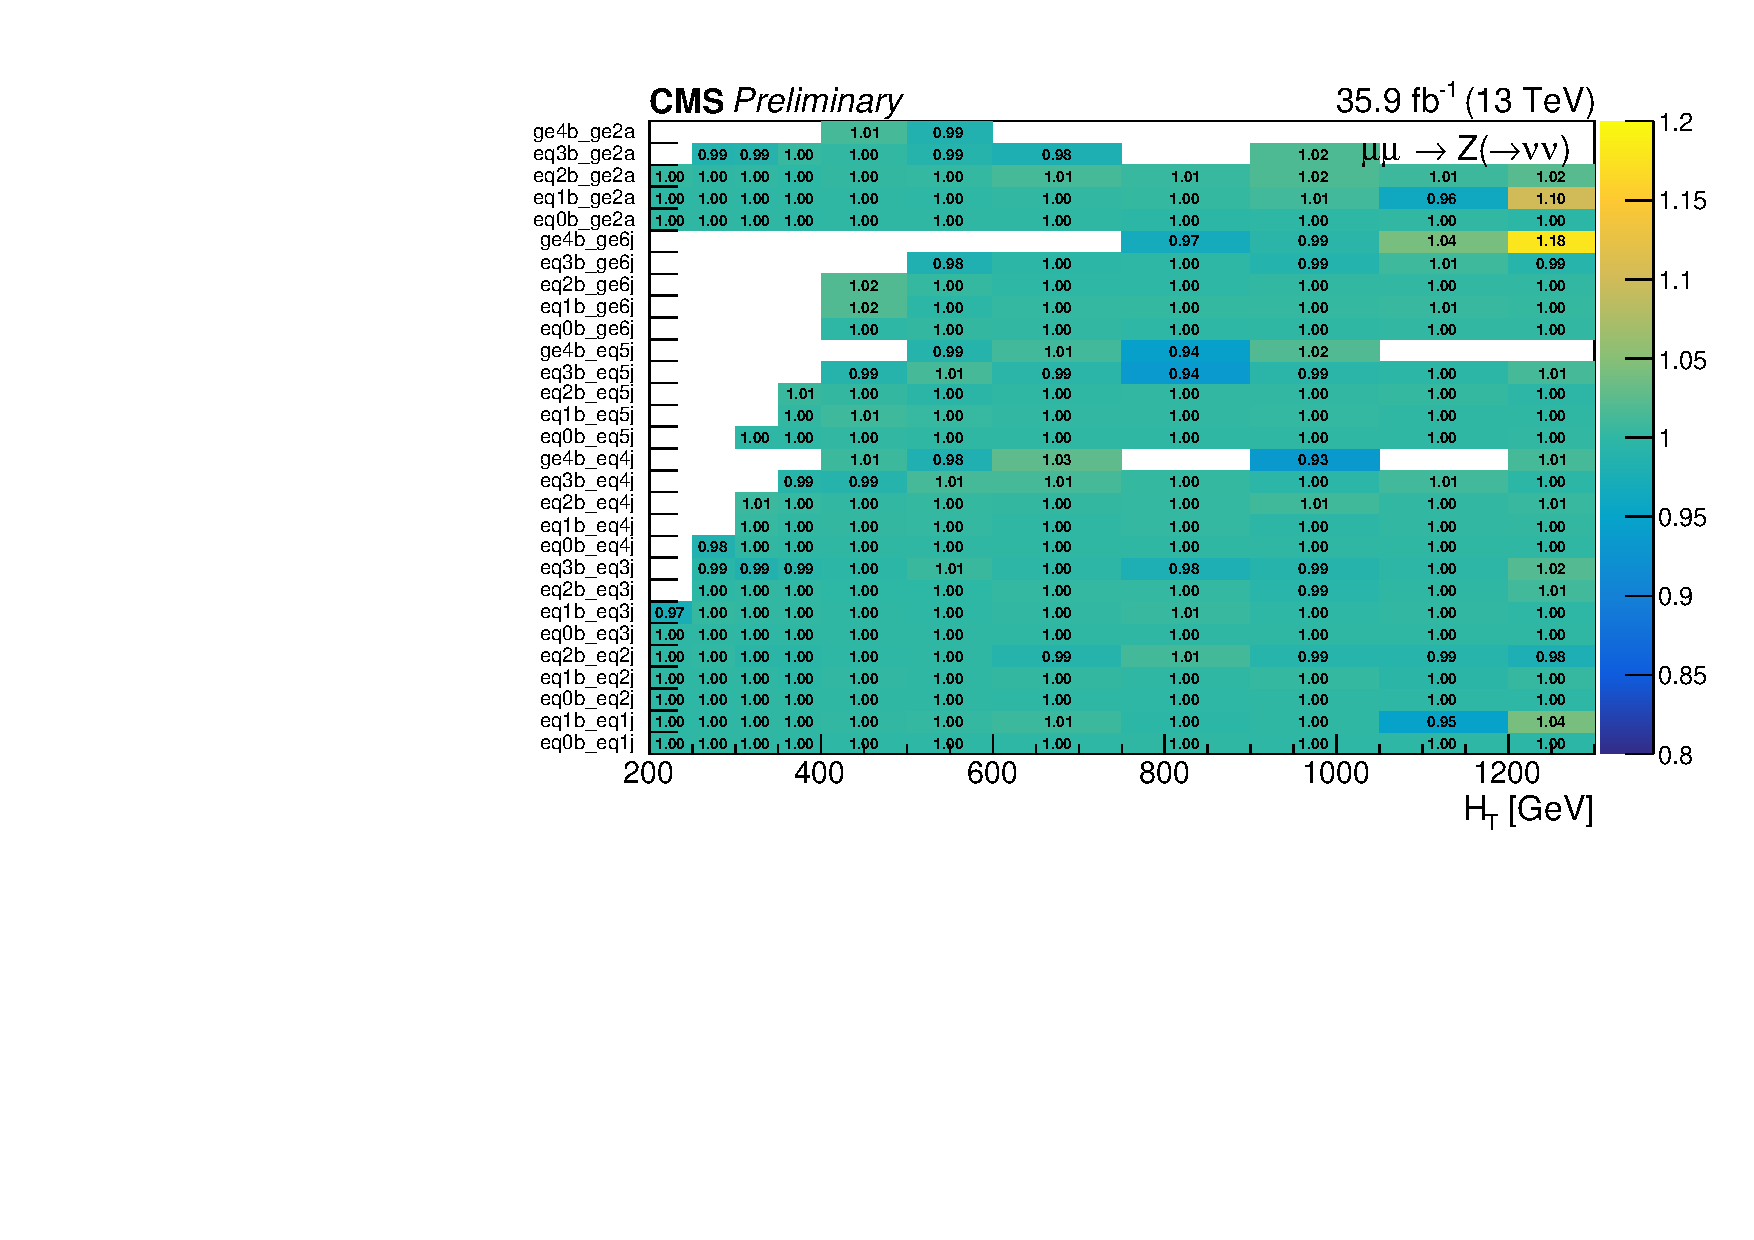
\includegraphics[width=0.5\textwidth]{figs/analysis/transferfactors/tfratio_mumu_Zinv_2d_bsfWeightUp}}~
	\subfloat{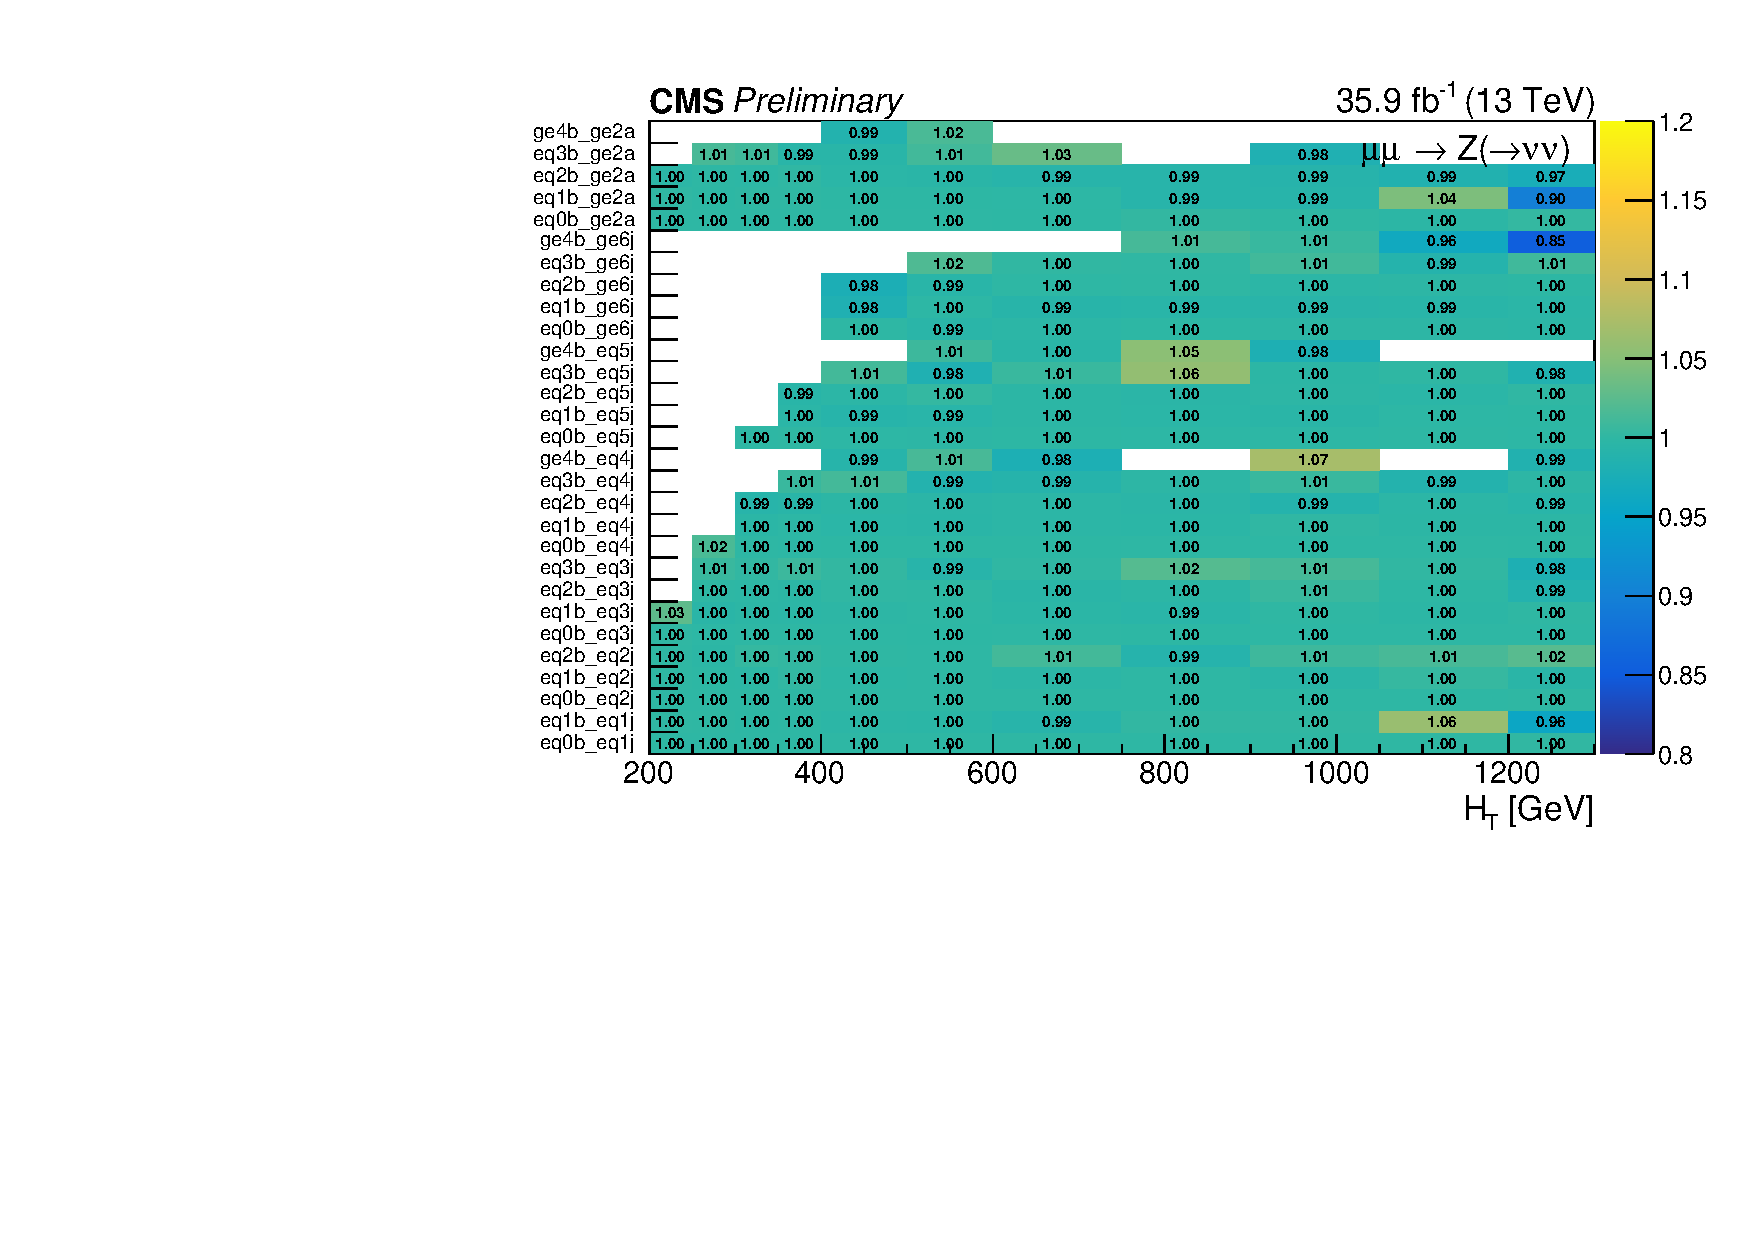
\includegraphics[width=0.5\textwidth]{figs/analysis/transferfactors/tfratio_mumu_Zinv_2d_bsfWeightDown}}\\
	\caption{The ratio of the \Tmutottw (top) and \Tmumutoz (bottom) transfer 
		factors in each \njnbht bin when varying the b-tagging correction 
		factors for bottom and charm quarks by $+1\sigma$ (left) and $-1\sigma$ 
		(right) with respect to 
		their nominal values.}
	\label{fig:tfvariations-btagging-heavy}
\end{figure}

\begin{figure}[h!]
	\subfloat{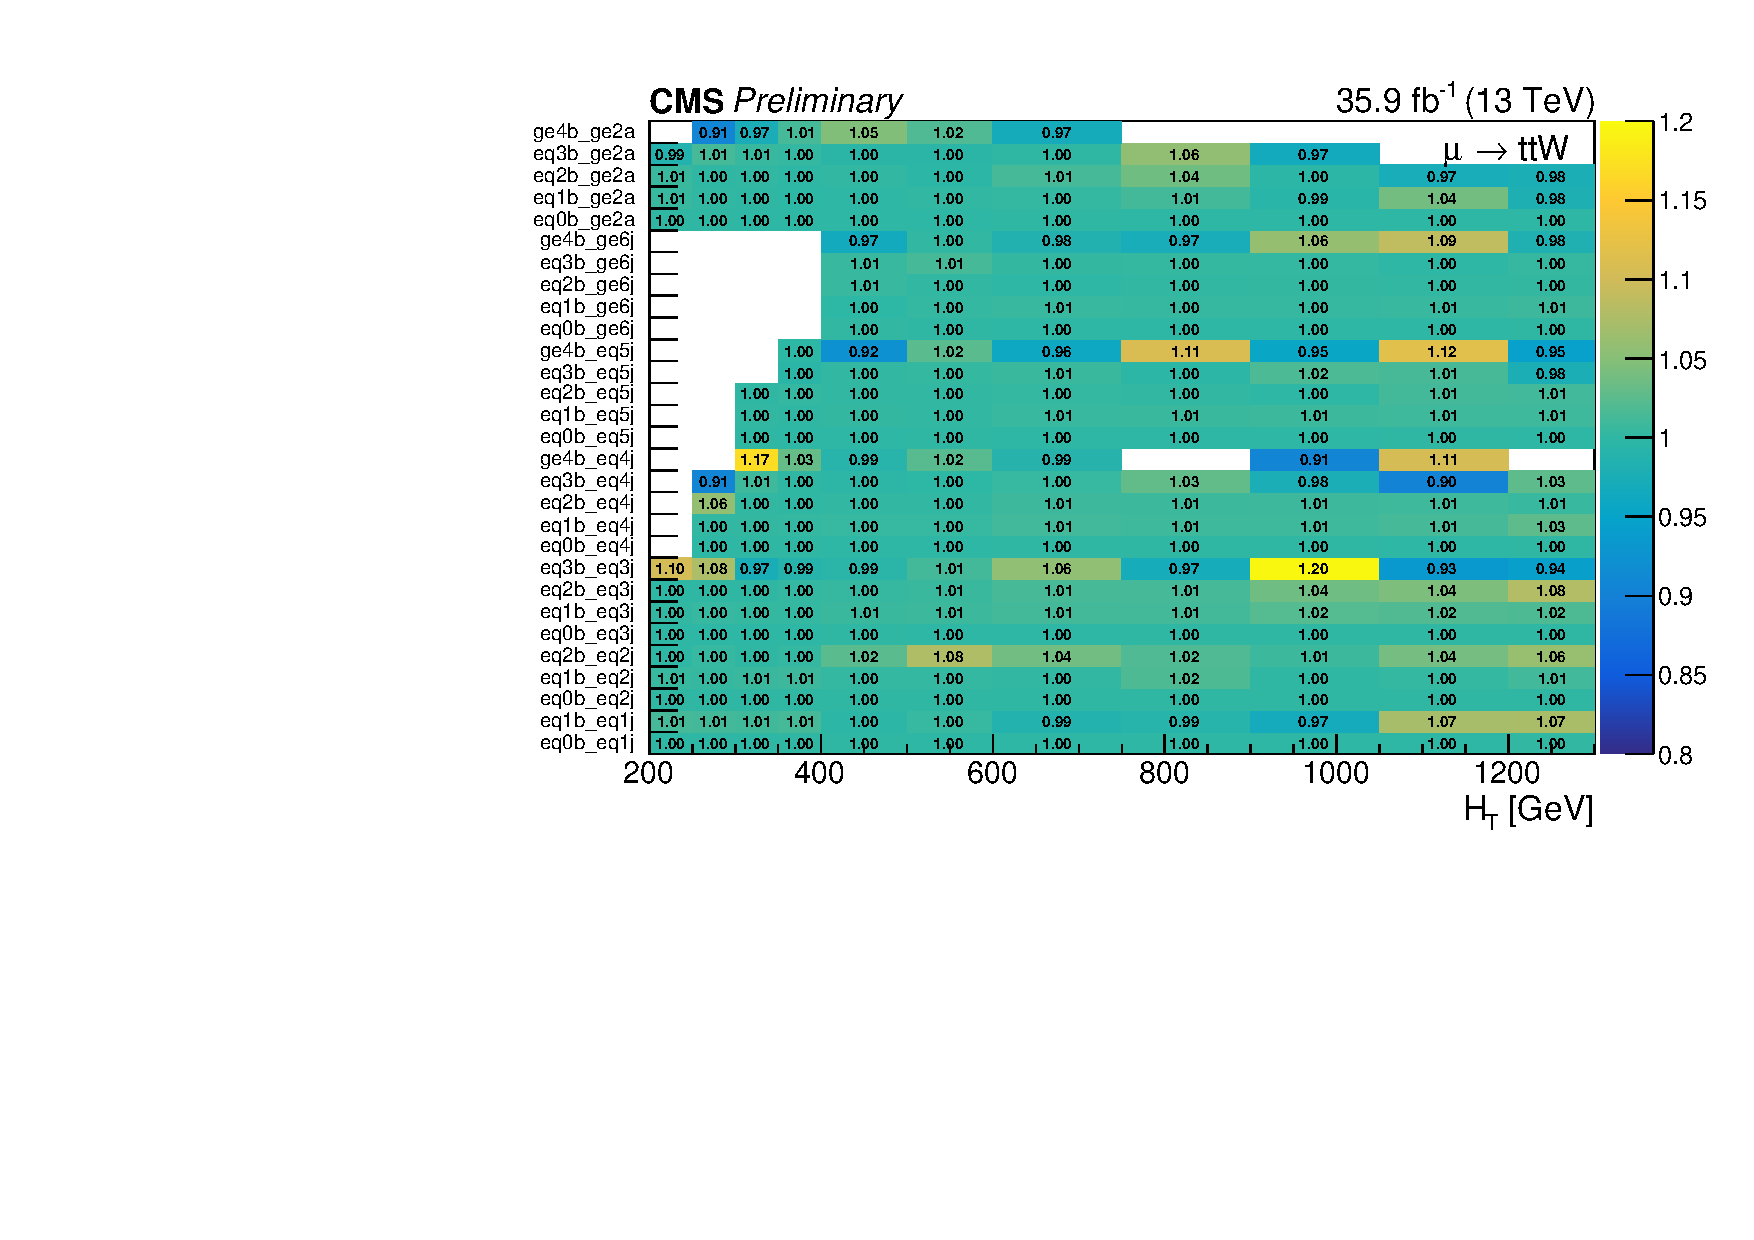
\includegraphics[width=0.5\textwidth]{figs/analysis/transferfactors/tfratio_mu_Ttw_2d_bsfLightWeightUp}}~
	\subfloat{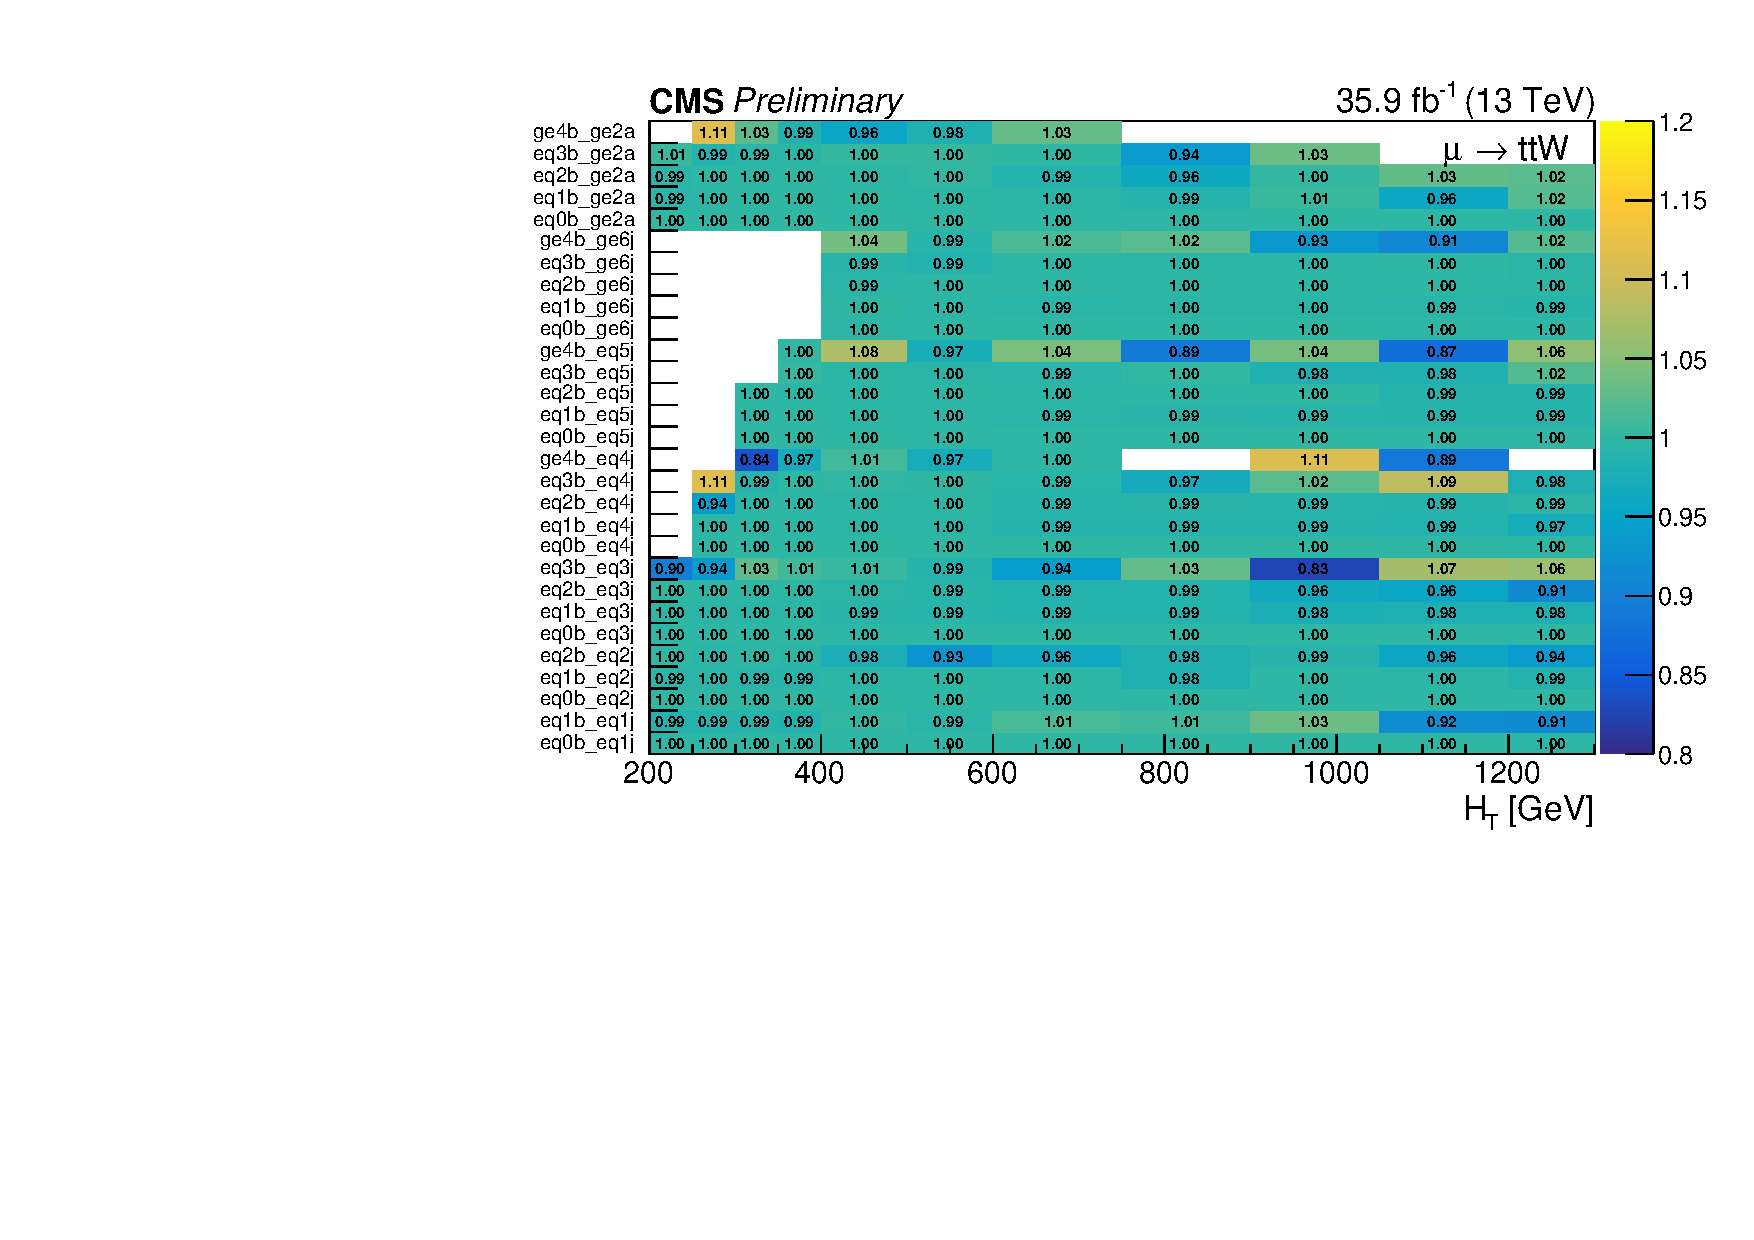
\includegraphics[width=0.5\textwidth]{figs/analysis/transferfactors/tfratio_mu_Ttw_2d_bsfLightWeightDown}}\\
	\subfloat{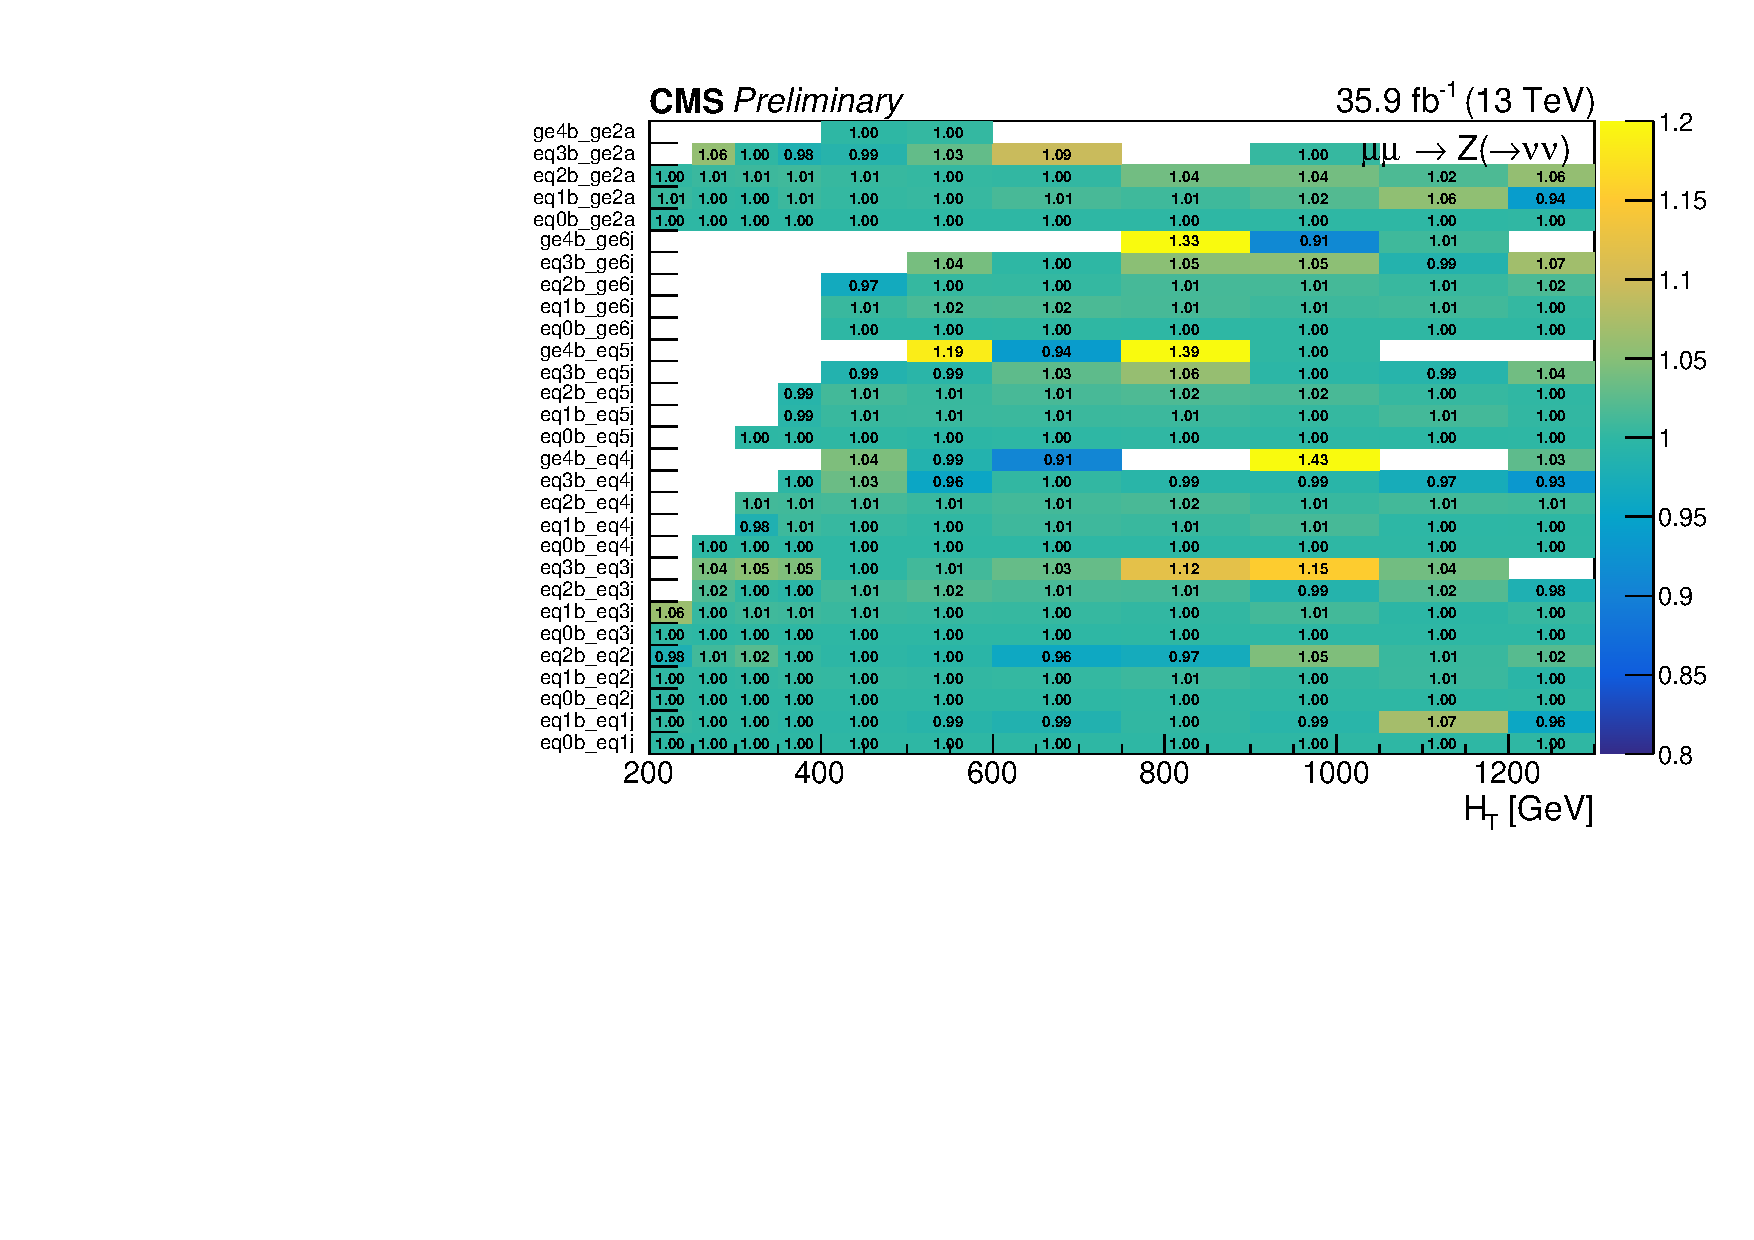
\includegraphics[width=0.5\textwidth]{figs/analysis/transferfactors/tfratio_mumu_Zinv_2d_bsfLightWeightUp}}~
	\subfloat{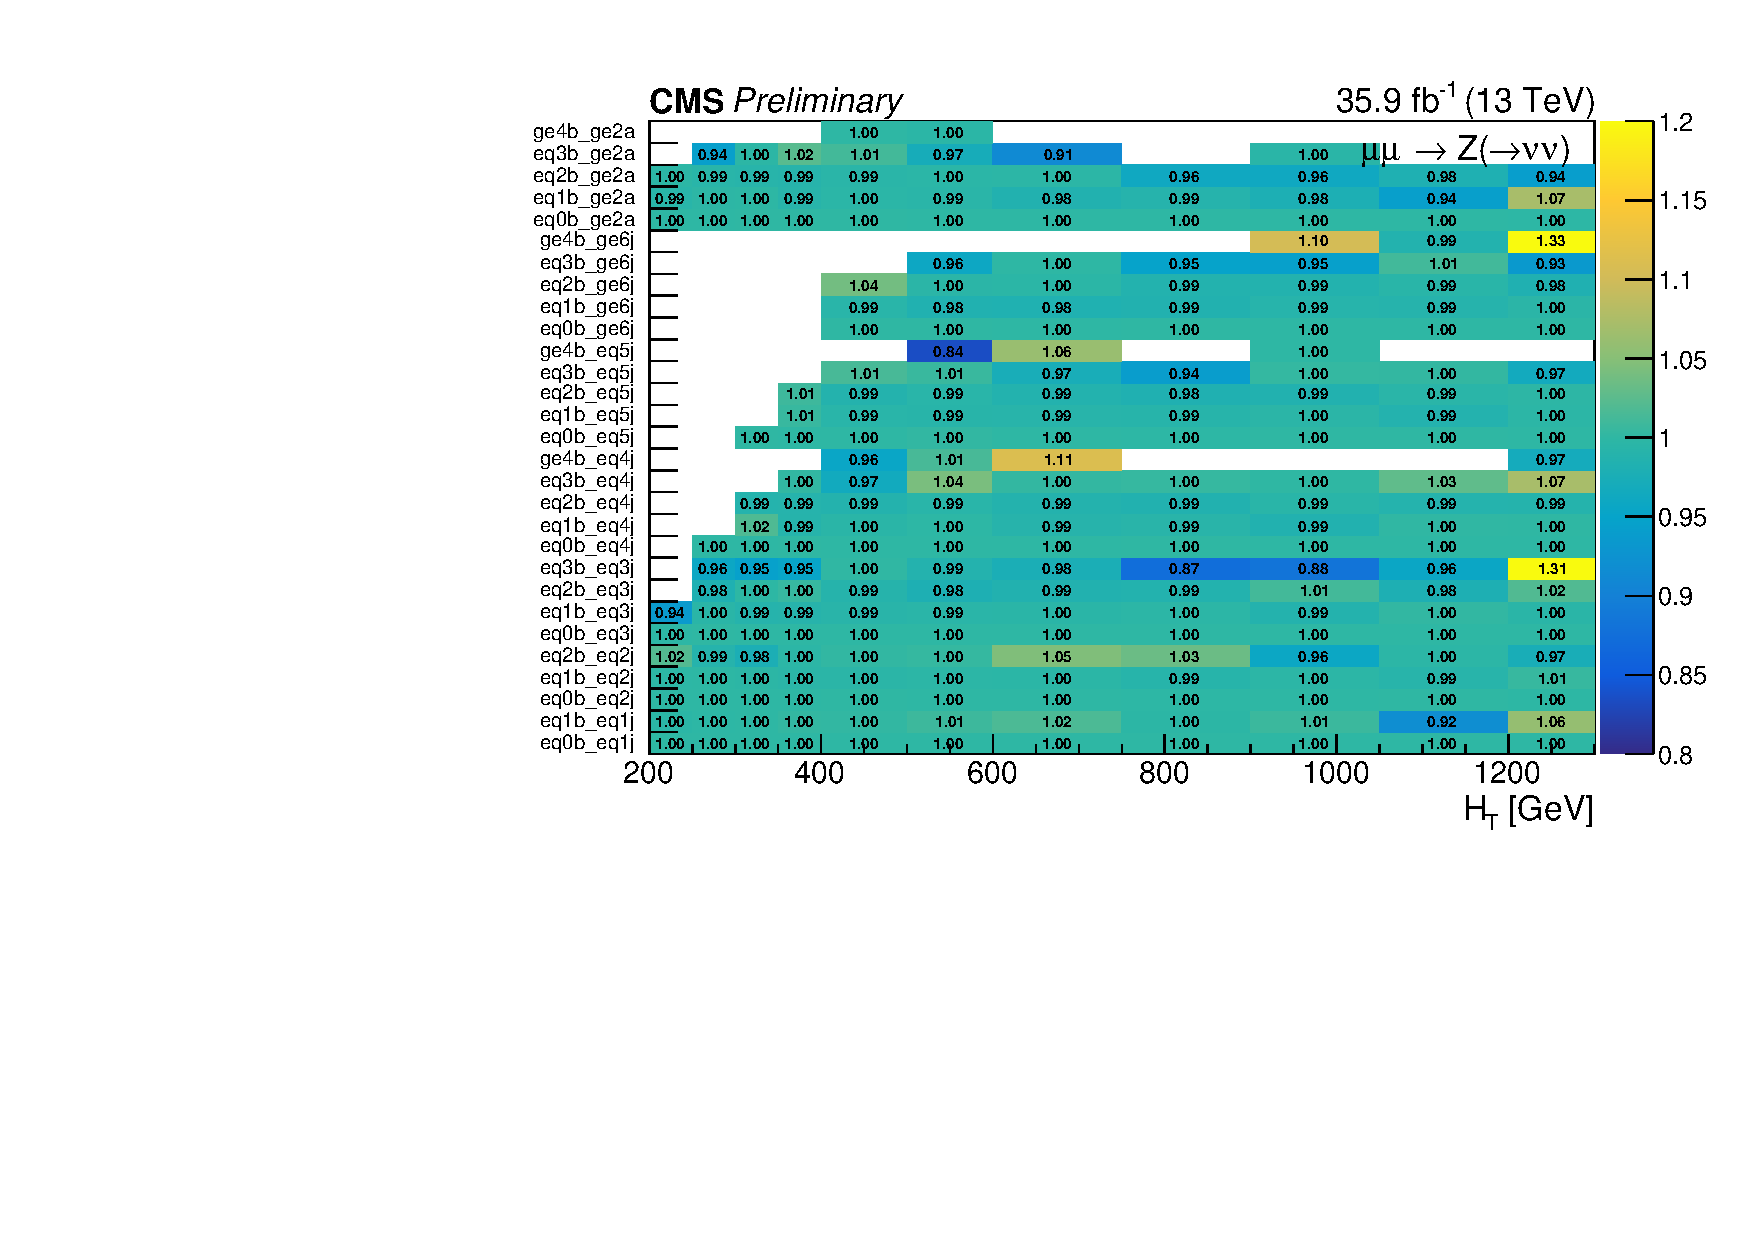
\includegraphics[width=0.5\textwidth]{figs/analysis/transferfactors/tfratio_mumu_Zinv_2d_bsfLightWeightDown}}\\
	\caption{The ratio of the \Tmutottw (top) and \Tmumutoz (bottom) transfer 
		factors in each \njnbht bin when varying the b-tagging correction 
		factors for light partons (u, d, s, gluon) by $+1\sigma$ (left) and 
		$-1\sigma$ (right) with respect to 
		their nominal values.}
	\label{fig:tfvariations-btagging-light}
\end{figure}

\begin{figure}[h!]
	\subfloat{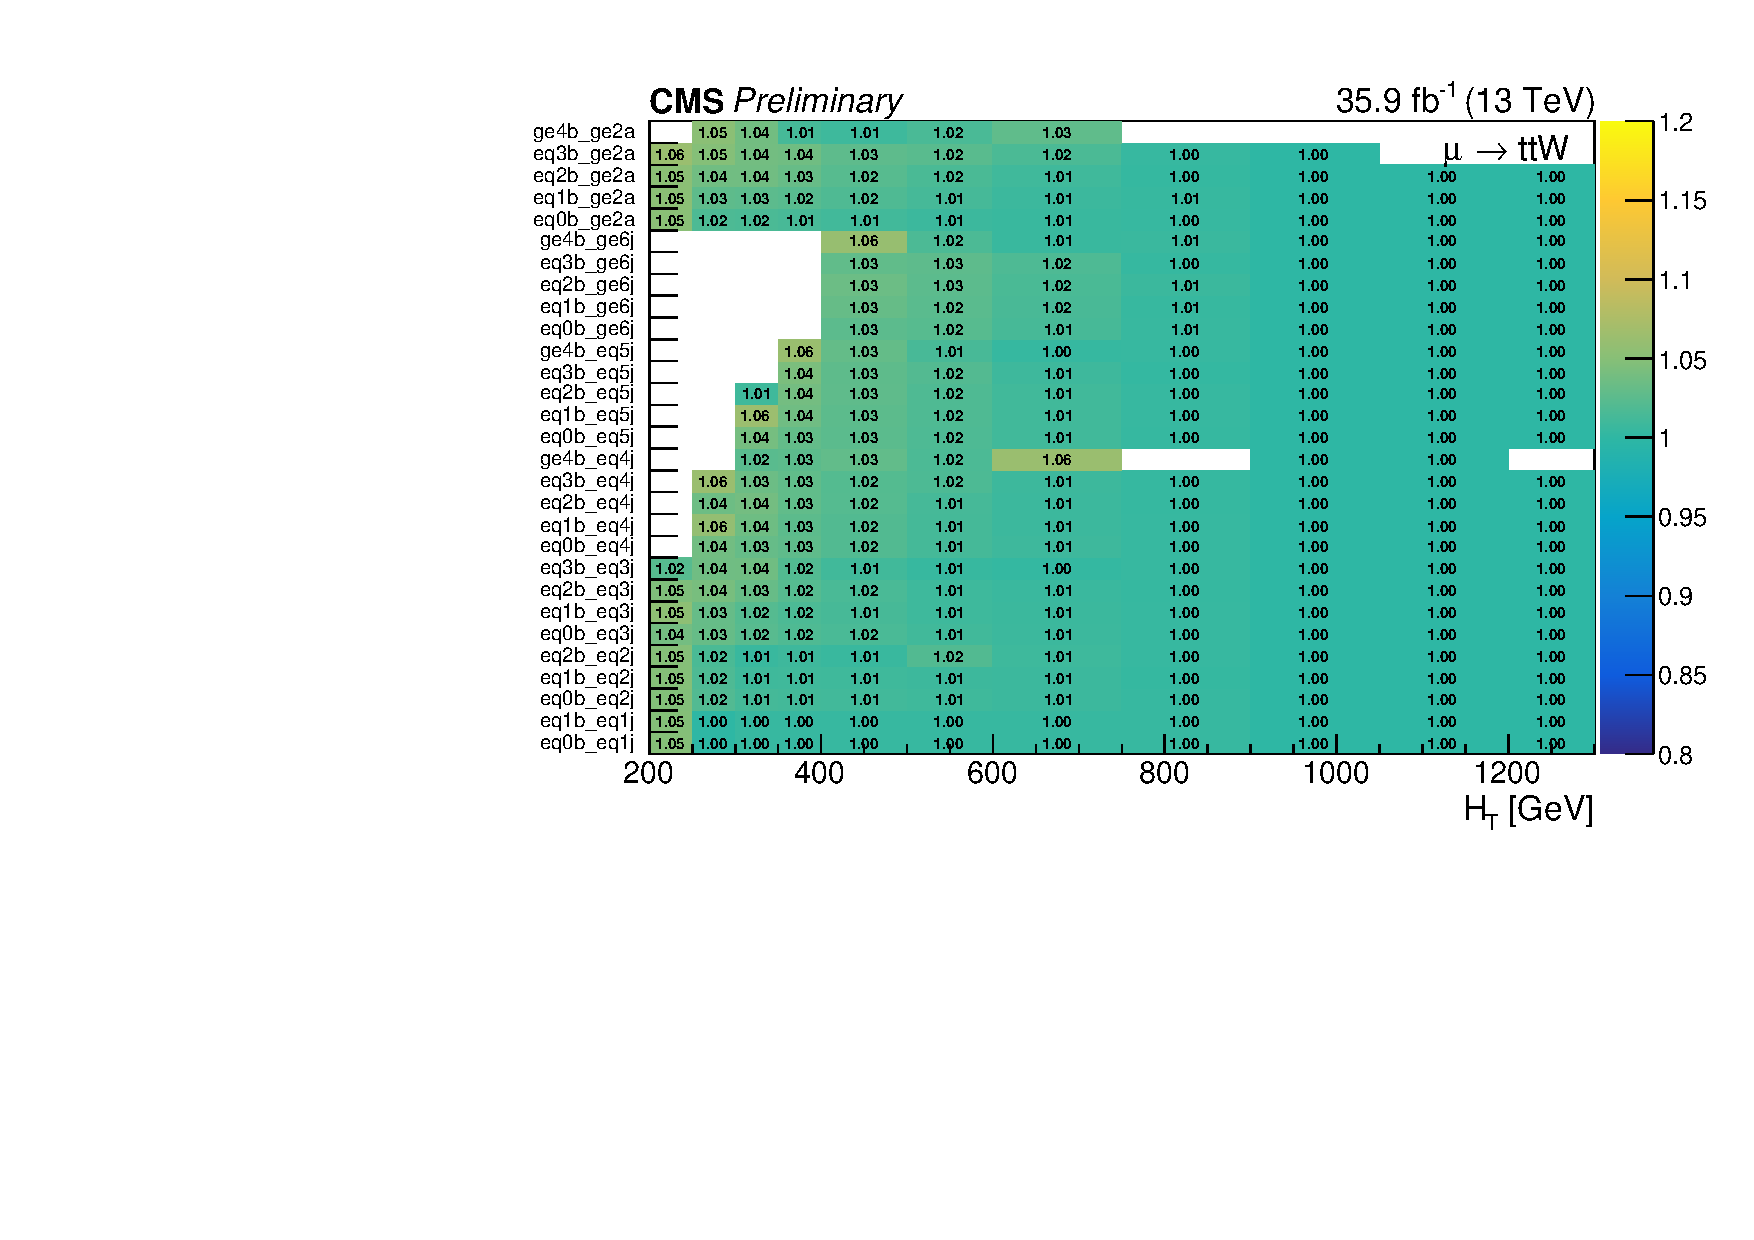
\includegraphics[width=0.5\textwidth]{figs/analysis/transferfactors/tfratio_mu_Ttw_2d_triggerWeightUp}}~
	\subfloat{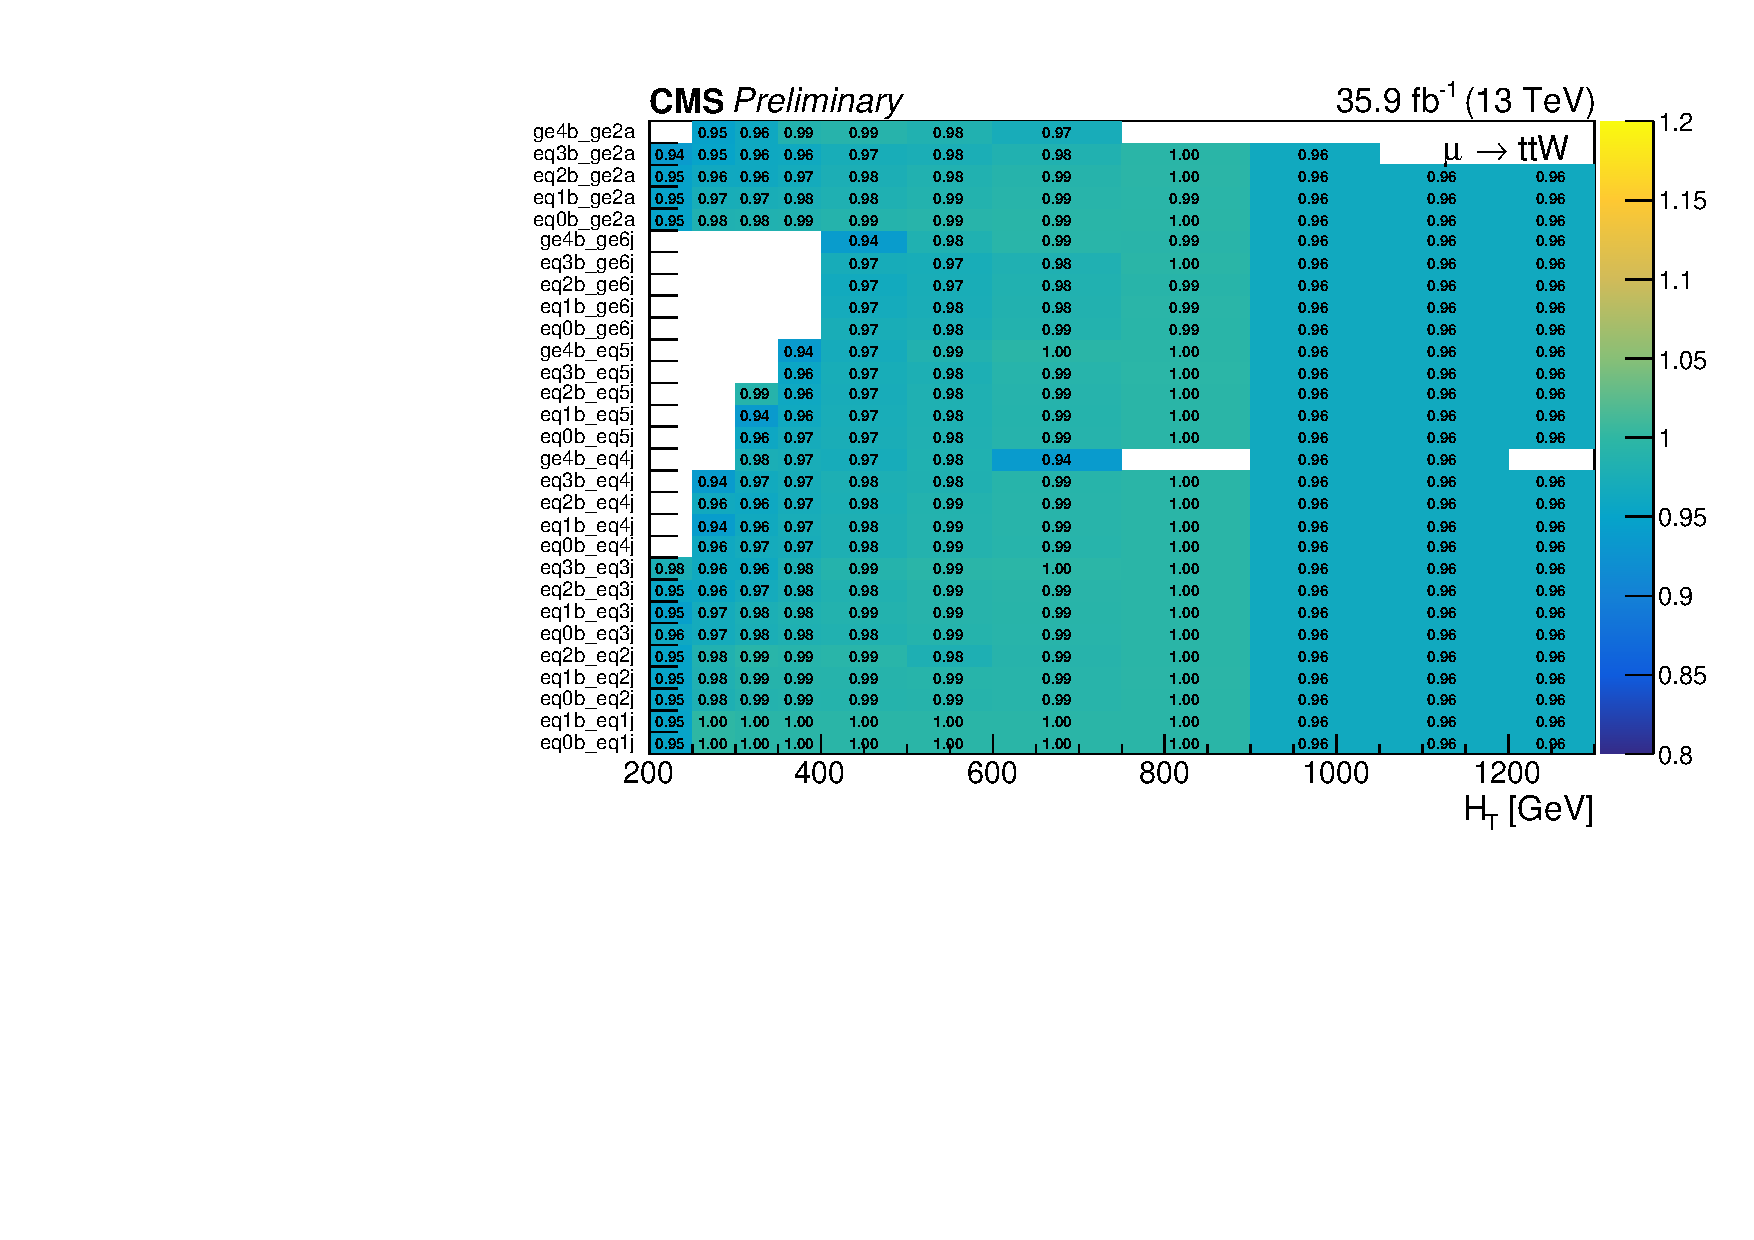
\includegraphics[width=0.5\textwidth]{figs/analysis/transferfactors/tfratio_mu_Ttw_2d_triggerWeightDown}}\\
	\subfloat{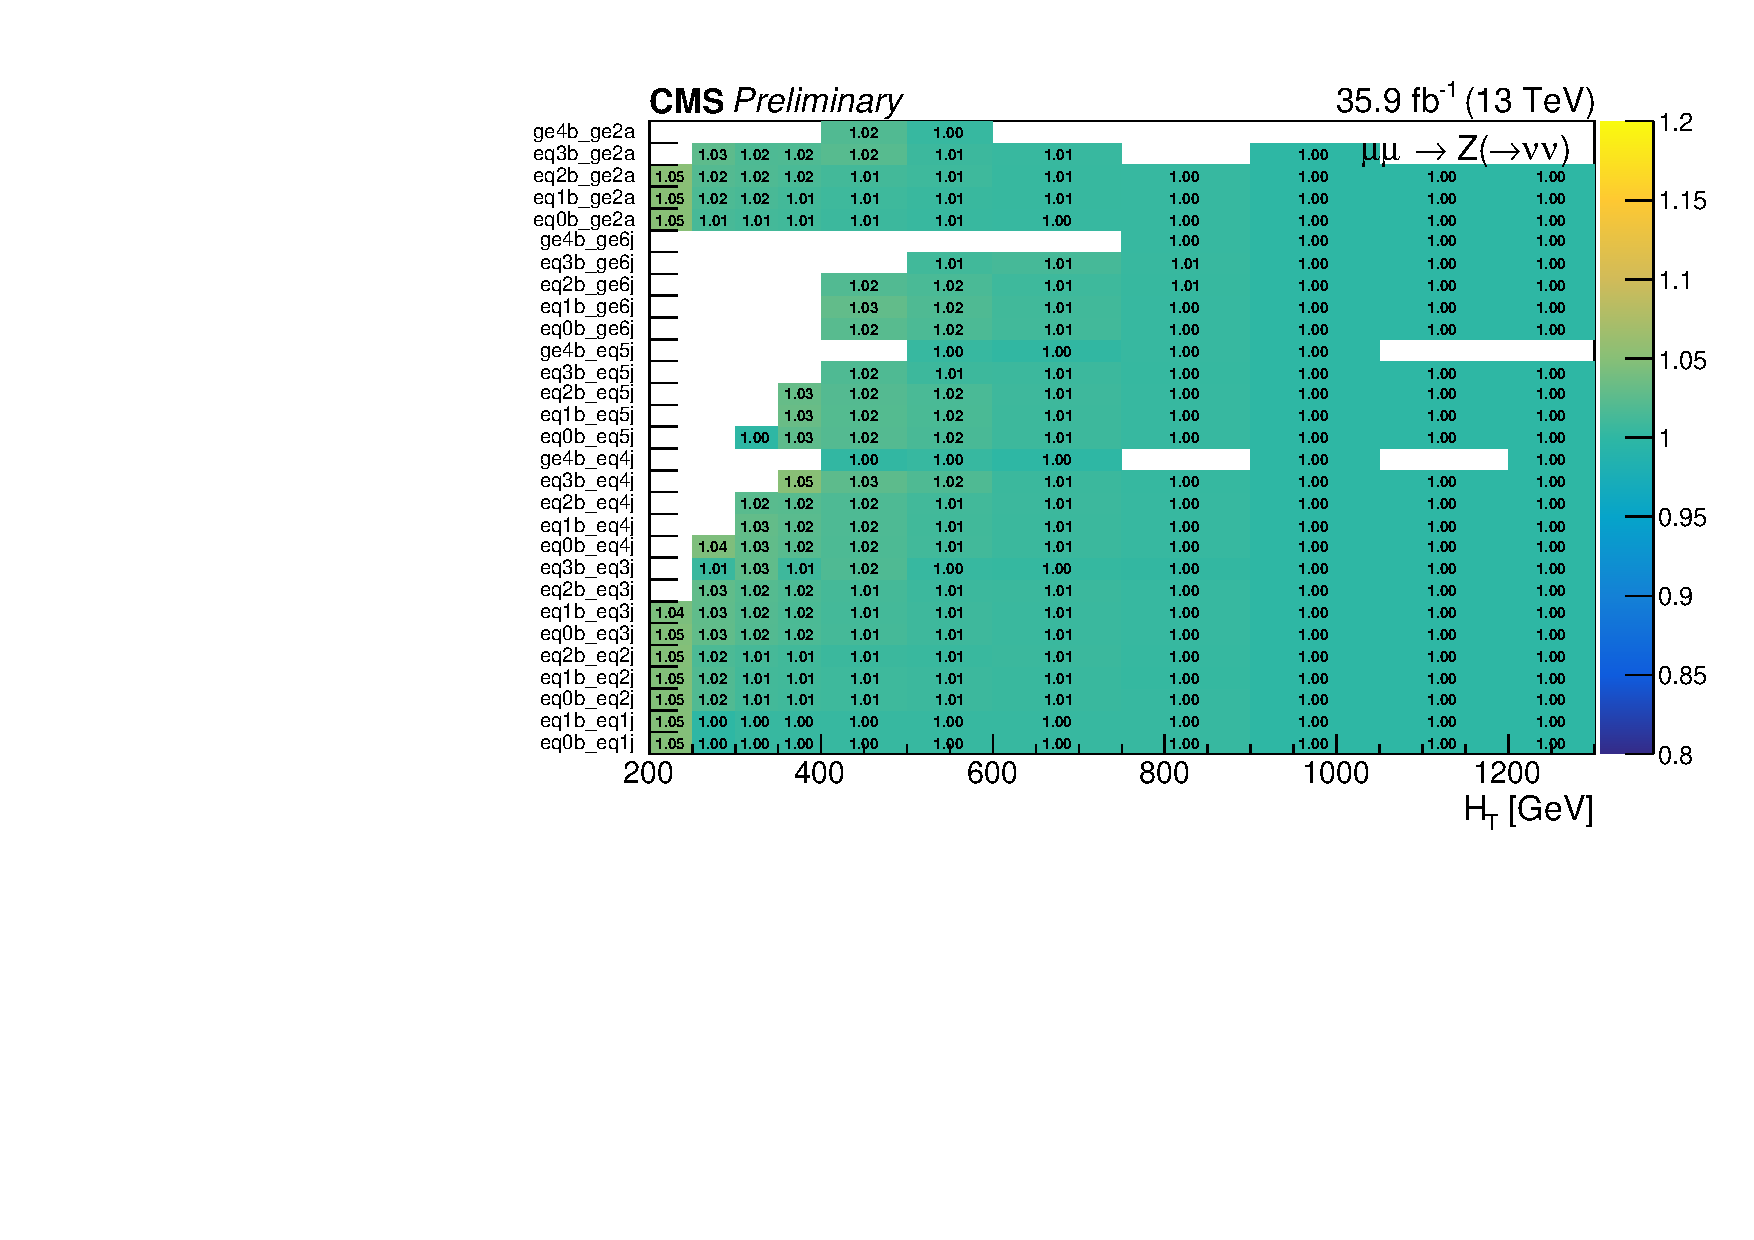
\includegraphics[width=0.5\textwidth]{figs/analysis/transferfactors/tfratio_mumu_Zinv_2d_triggerWeightUp}}~
	\subfloat{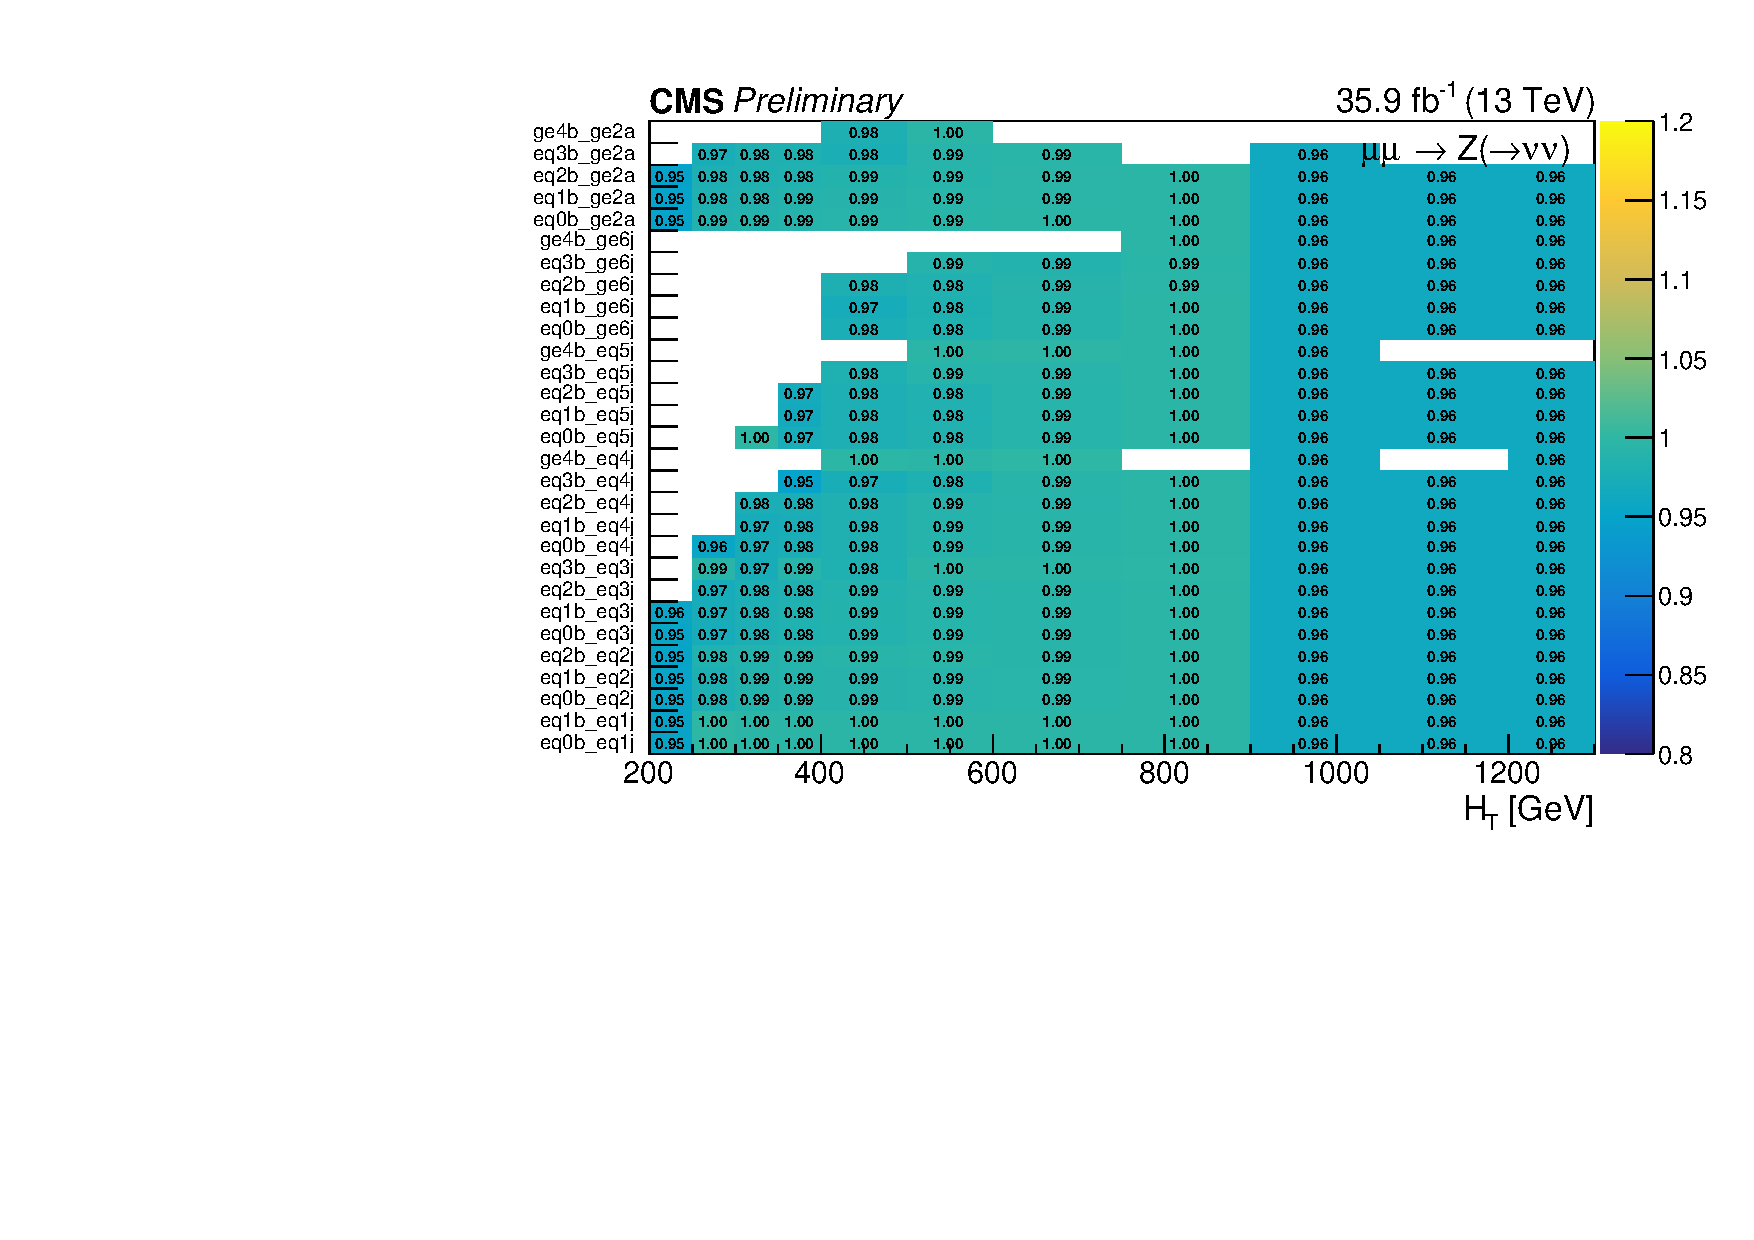
\includegraphics[width=0.5\textwidth]{figs/analysis/transferfactors/tfratio_mumu_Zinv_2d_triggerWeightDown}}\\
	\caption{The ratio of the \Tmutottw (top) and \Tmumutoz (bottom) transfer 
		factors in each \njnbht bin when varying the trigger correction factors 
		by $+1\sigma$ (left) and $-1\sigma$ (right) with respect to 
		their nominal values.}
	\label{fig:tfvariations-trigger}
\end{figure}

\begin{figure}[h!]
	\subfloat{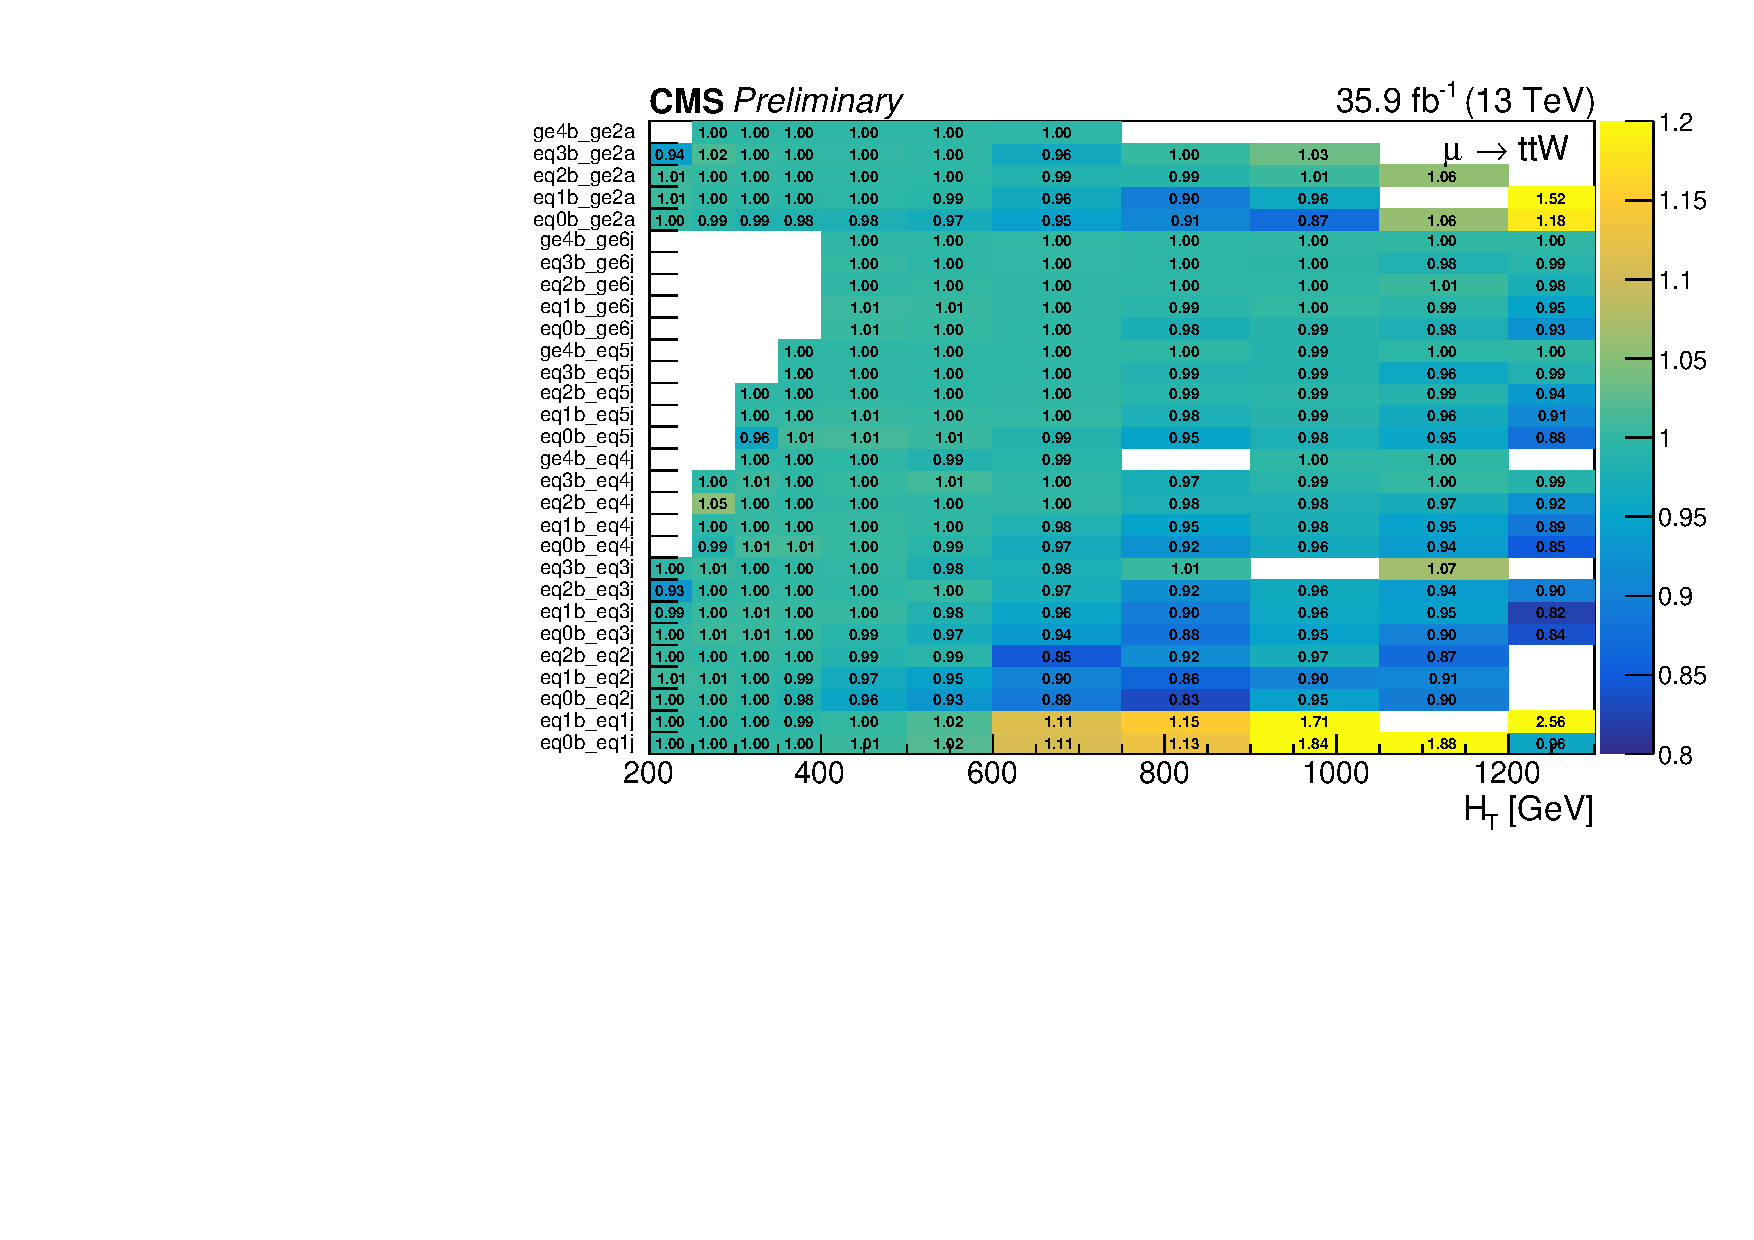
\includegraphics[width=0.5\textwidth]{figs/analysis/transferfactors/tfratio_mu_Ttw_2d_bosonPtWeightUp}}~
	\subfloat{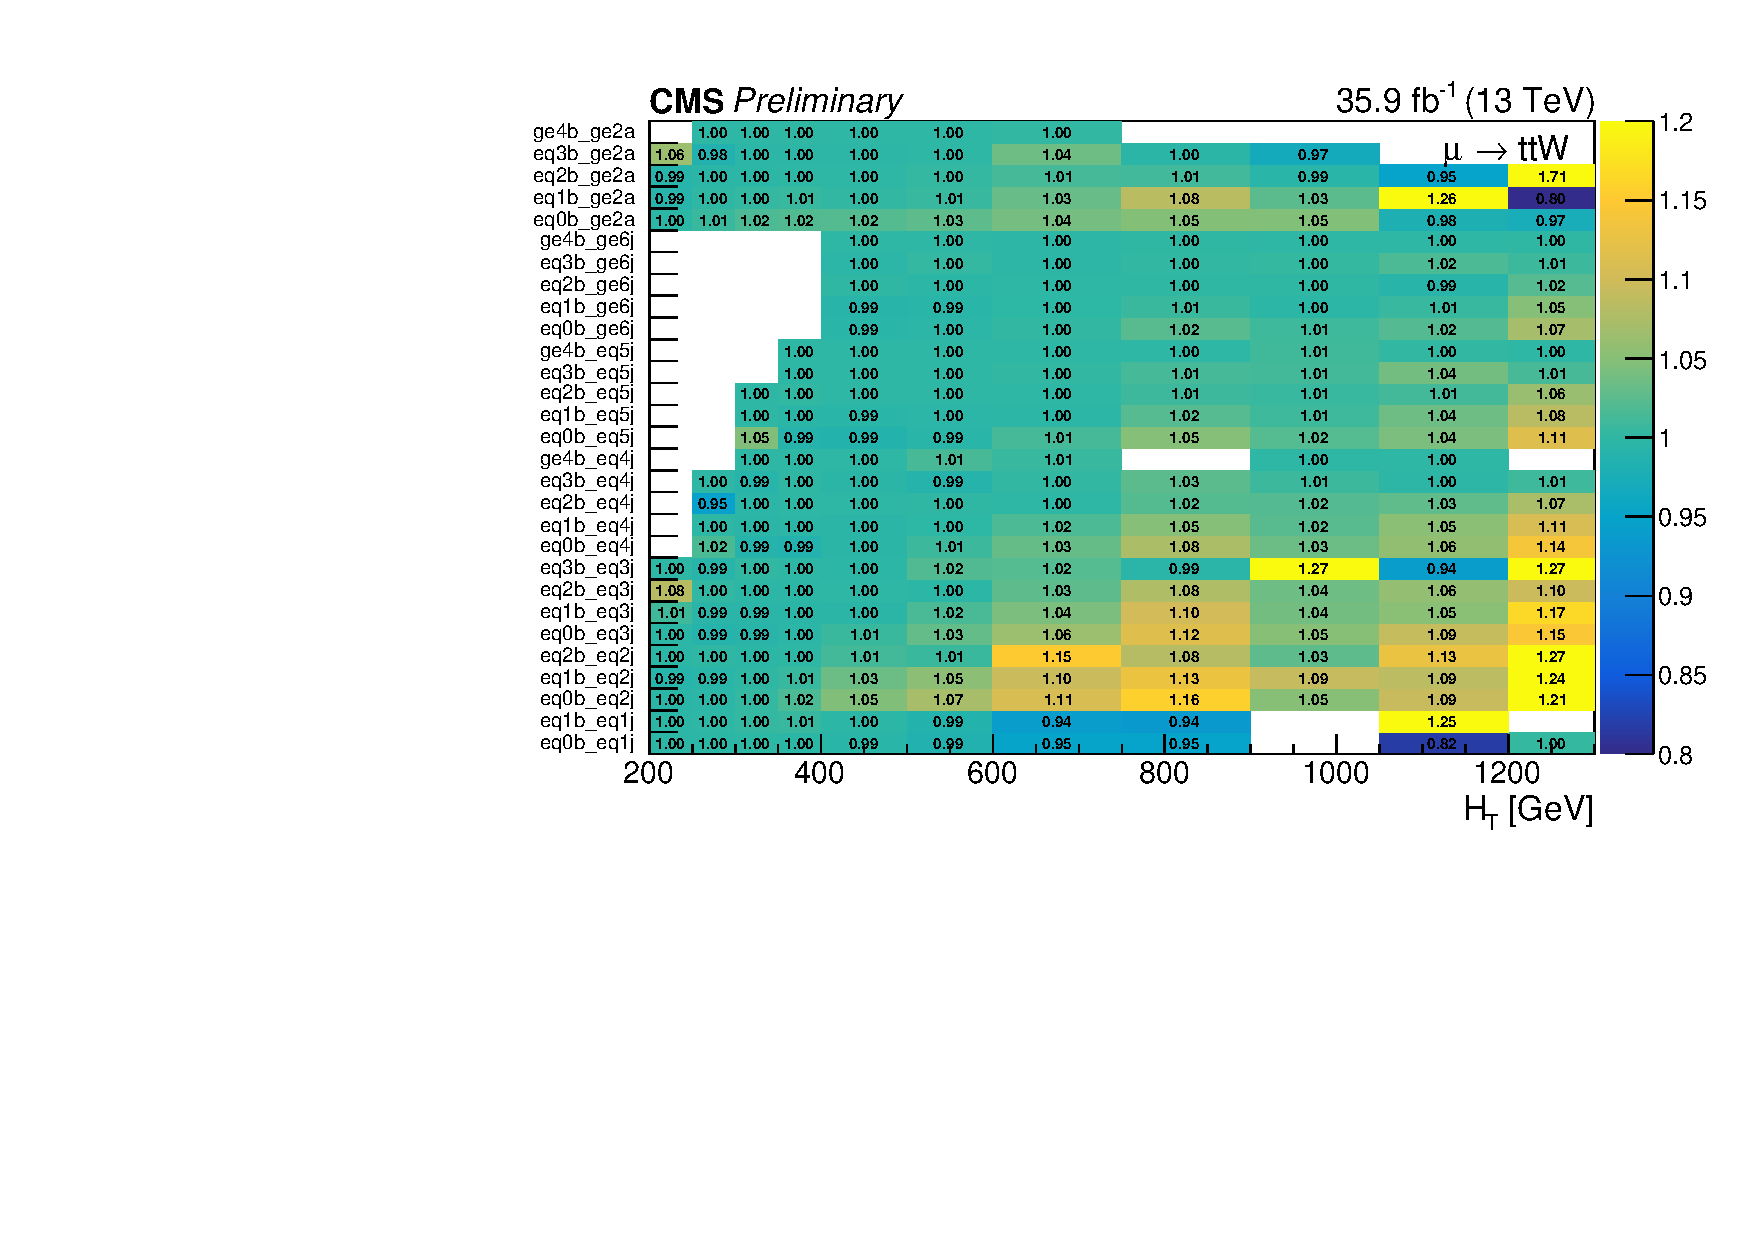
\includegraphics[width=0.5\textwidth]{figs/analysis/transferfactors/tfratio_mu_Ttw_2d_bosonPtWeightDown}}\\
	\subfloat{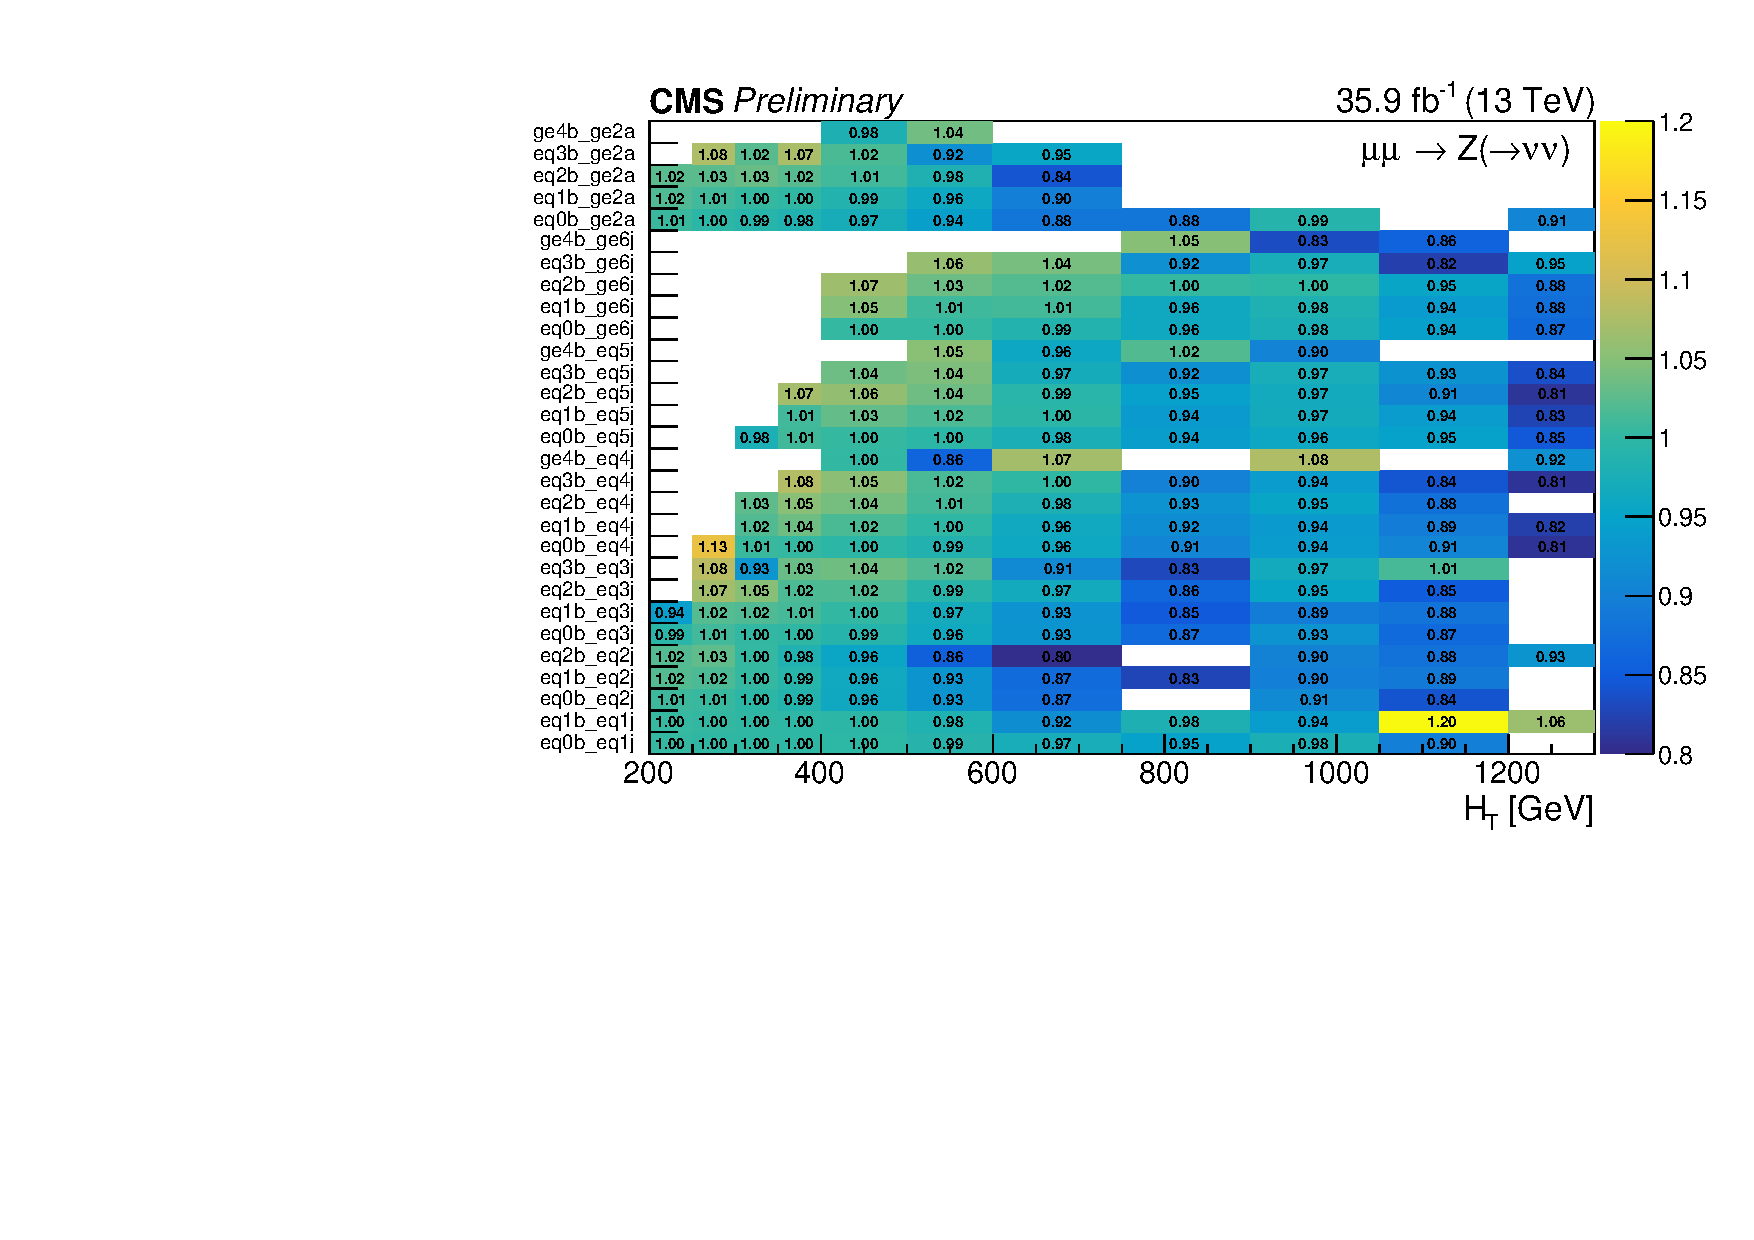
\includegraphics[width=0.5\textwidth]{figs/analysis/transferfactors/tfratio_mumu_Zinv_2d_bosonPtWeightUp}}~
	\subfloat{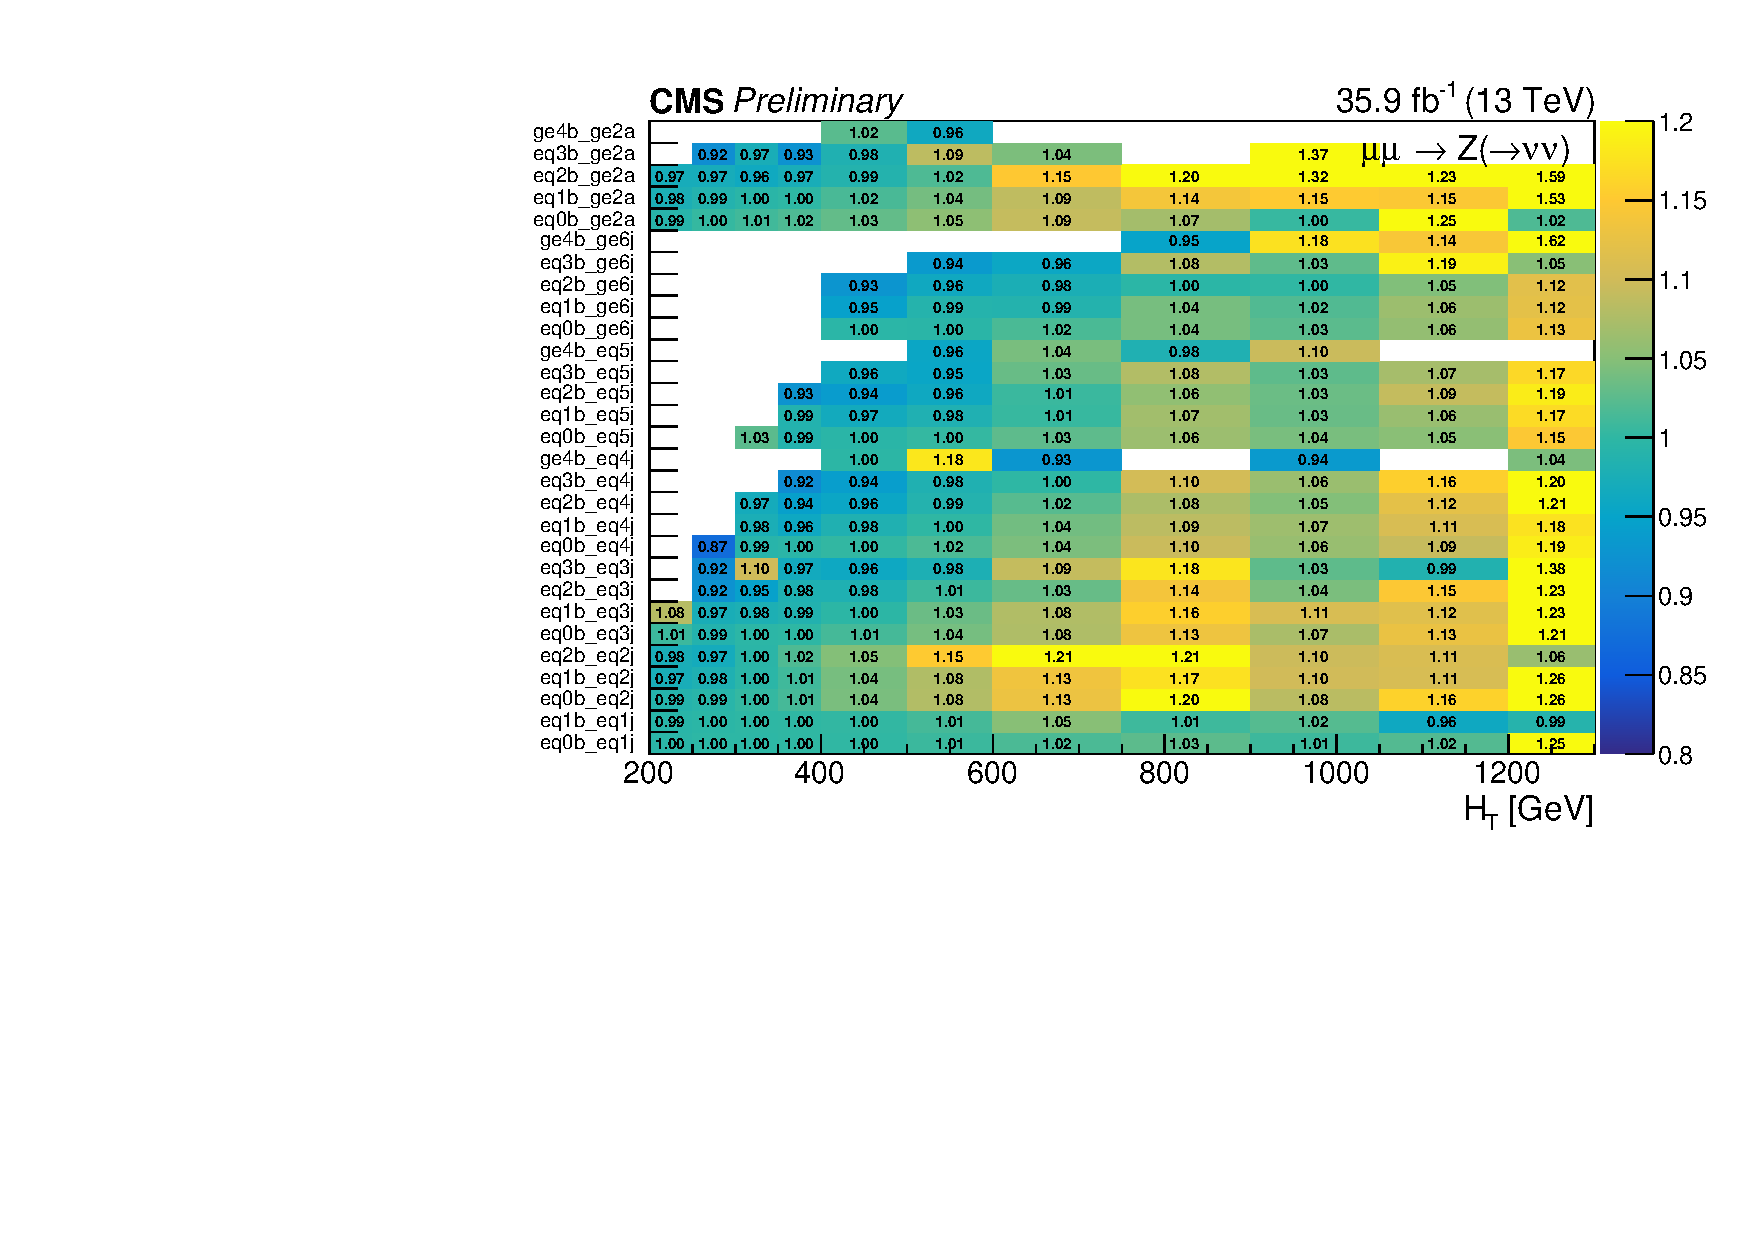
\includegraphics[width=0.5\textwidth]{figs/analysis/transferfactors/tfratio_mumu_Zinv_2d_bosonPtWeightDown}}\\
	\caption{The ratio of the \Tmutottw (top) and \Tmumutoz (bottom) transfer 
		factors in each \njnbht bin when varying the boson \pt dependent NLO 
		correction factors by $+1\sigma$ (left) and $-1\sigma$ (right) with 
		respect to 
		their nominal values.}
	\label{fig:tfvariations-nlo}
\end{figure}

\begin{figure}[h!]
	\subfloat{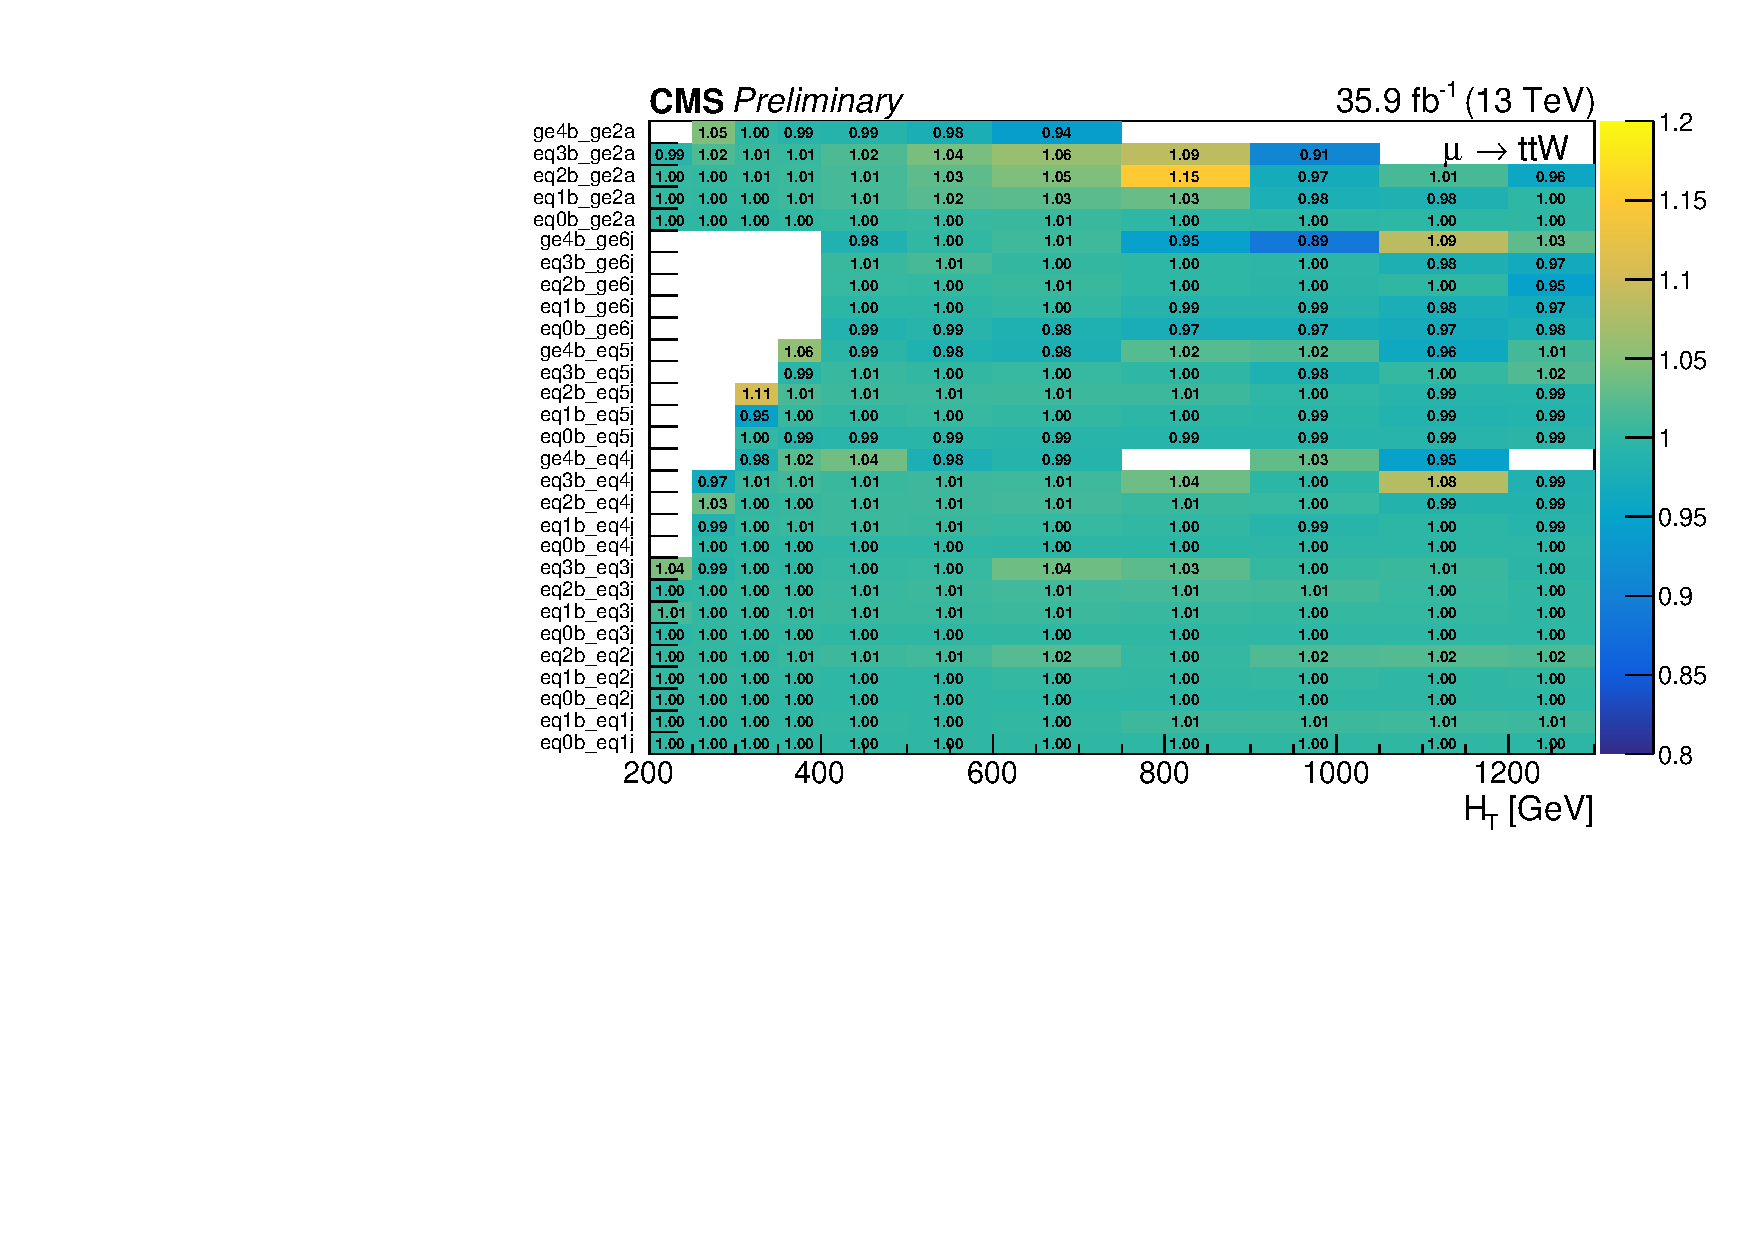
\includegraphics[width=0.5\textwidth]{figs/analysis/transferfactors/tfratio_mu_Ttw_2d_nIsrWeightUp}}~
	\subfloat{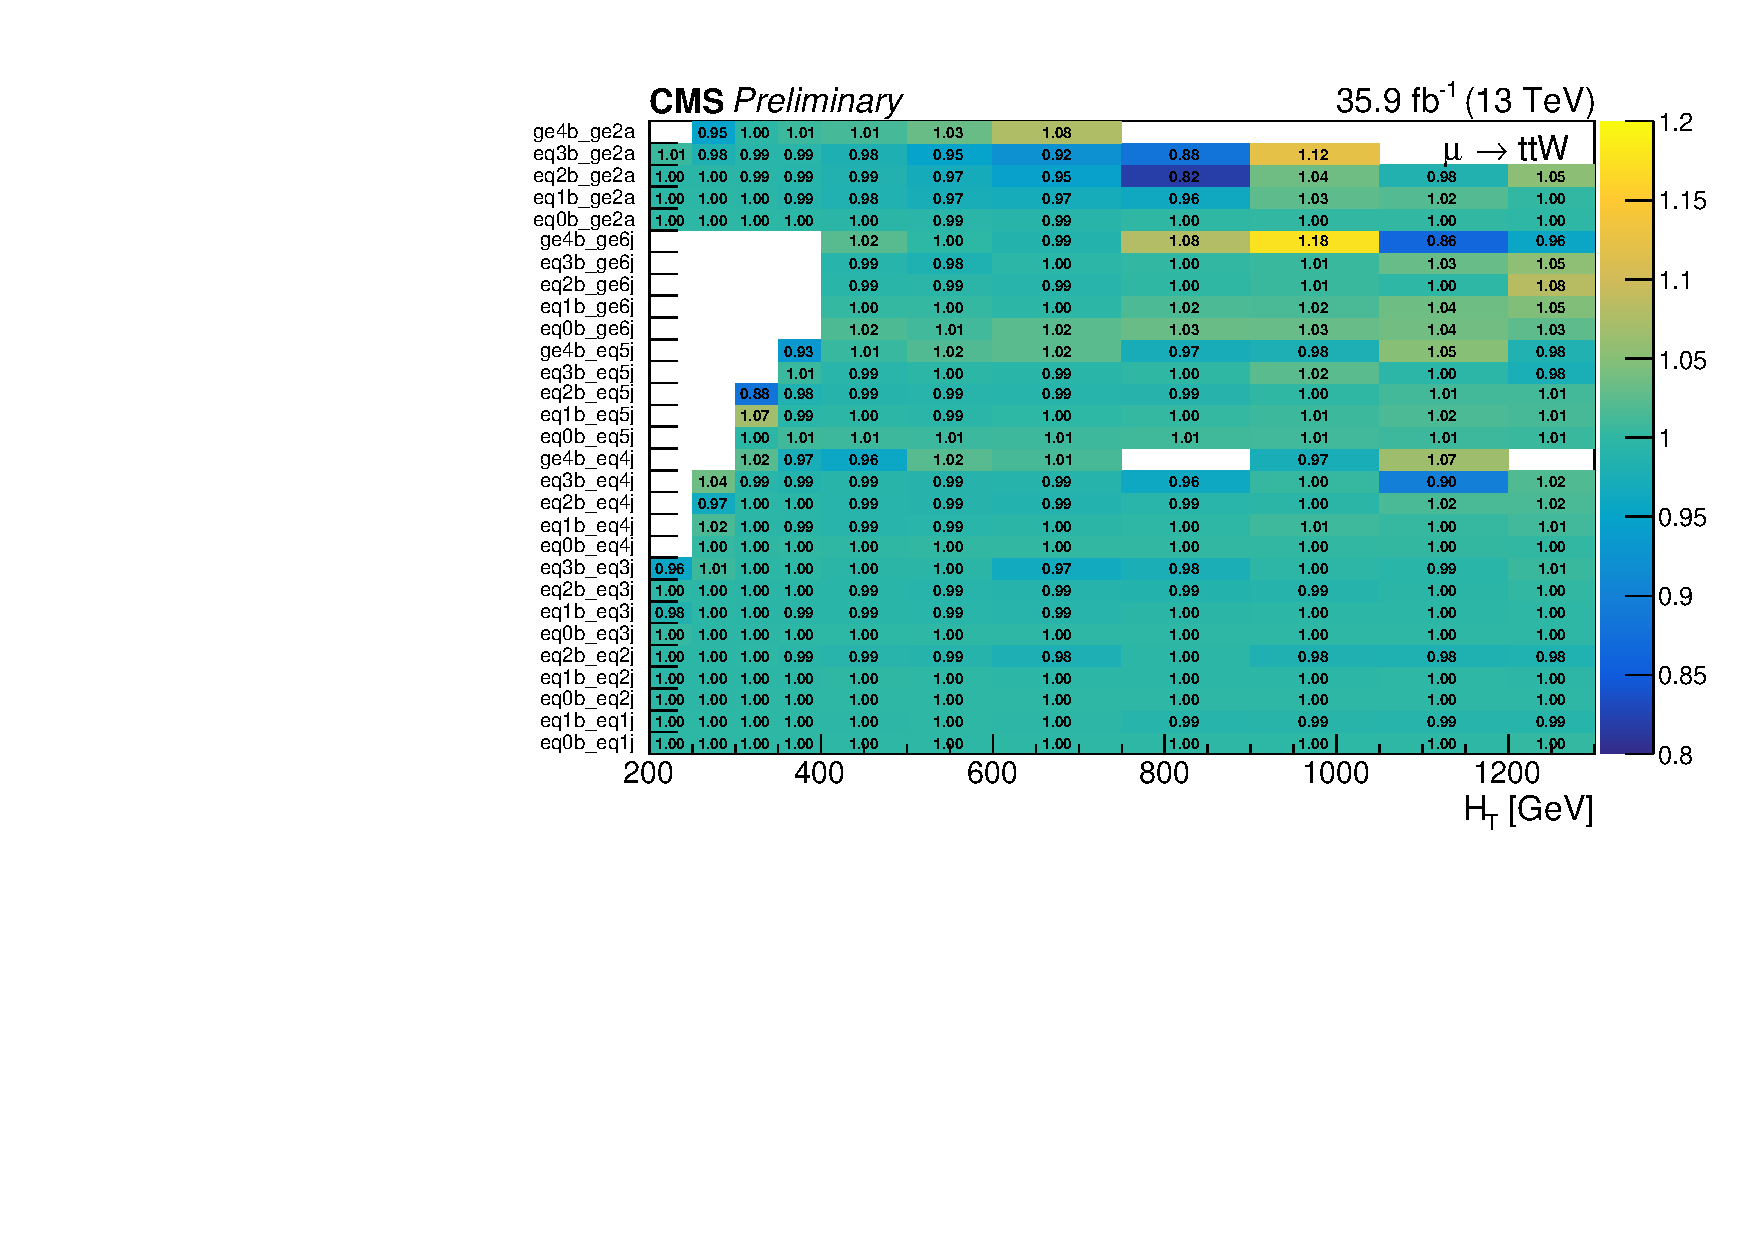
\includegraphics[width=0.5\textwidth]{figs/analysis/transferfactors/tfratio_mu_Ttw_2d_nIsrWeightDown}}\\
	\subfloat{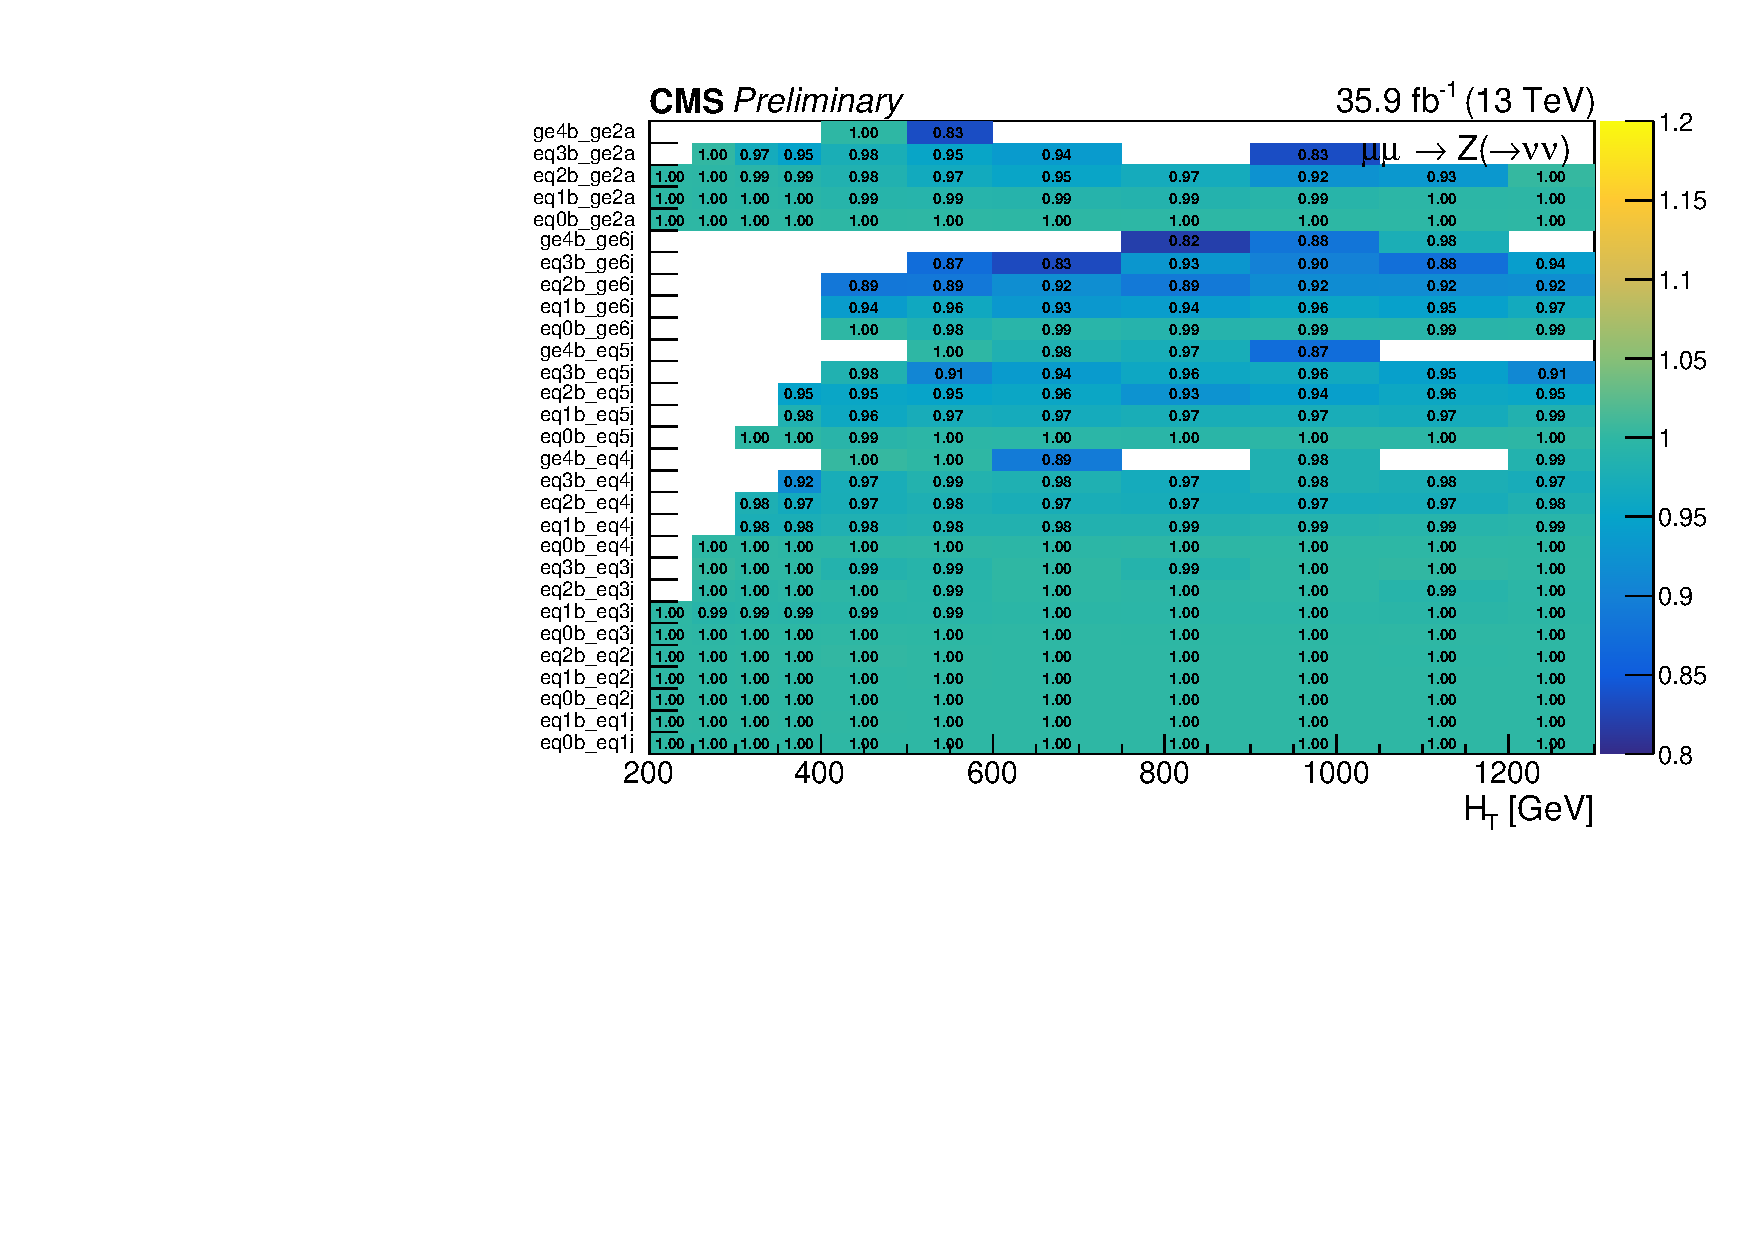
\includegraphics[width=0.5\textwidth]{figs/analysis/transferfactors/tfratio_mumu_Zinv_2d_nIsrWeightUp}}~
	\subfloat{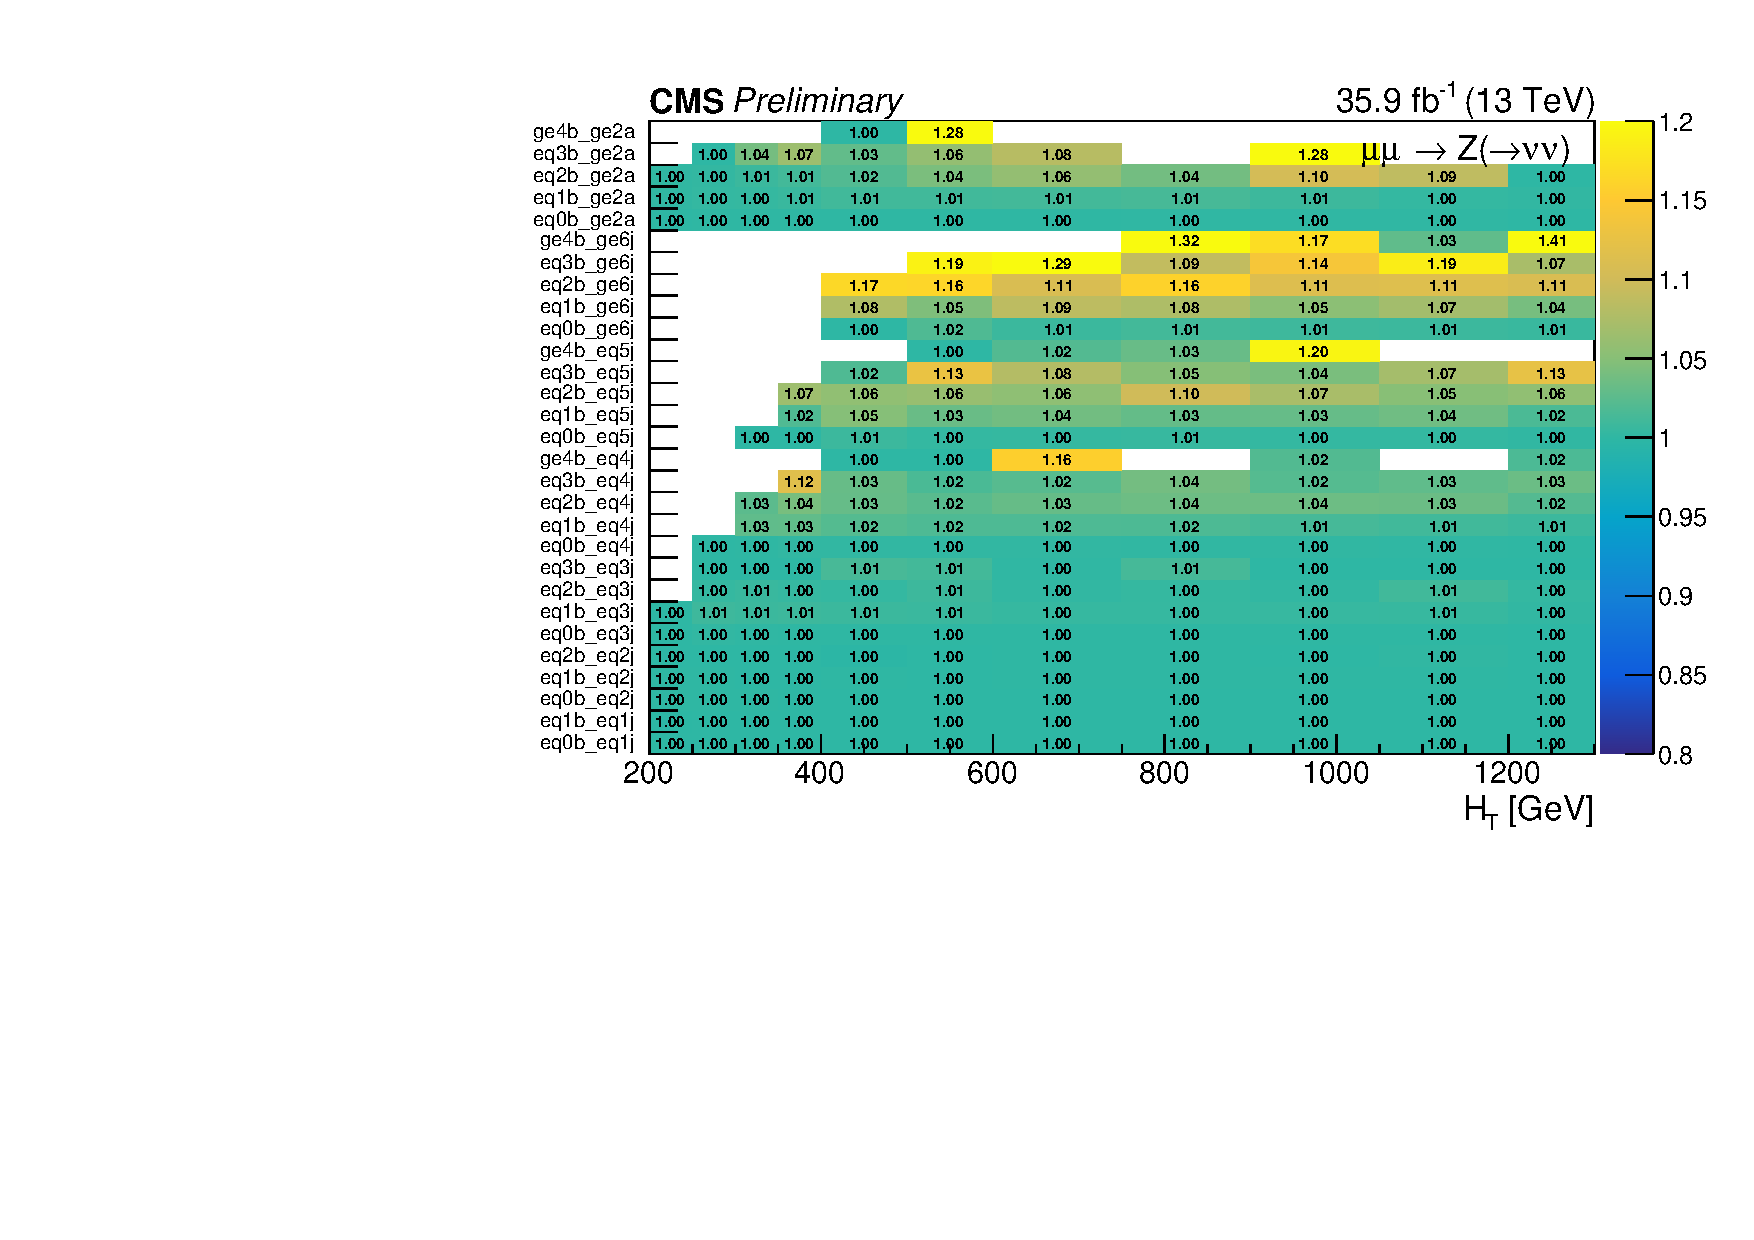
\includegraphics[width=0.5\textwidth]{figs/analysis/transferfactors/tfratio_mumu_Zinv_2d_nIsrWeightDown}}\\
	\caption{The ratio of the \Tmutottw (top) and \Tmumutoz (bottom) transfer 
		factors in each \njnbht bin when varying the \ttbar ISR correction 
		factors by $+1\sigma$ (left) and $-1\sigma$ (right) with respect to 
		their nominal values.}
	\label{fig:tfvariations-nisr}
\end{figure}

\begin{figure}[h!]
	\subfloat{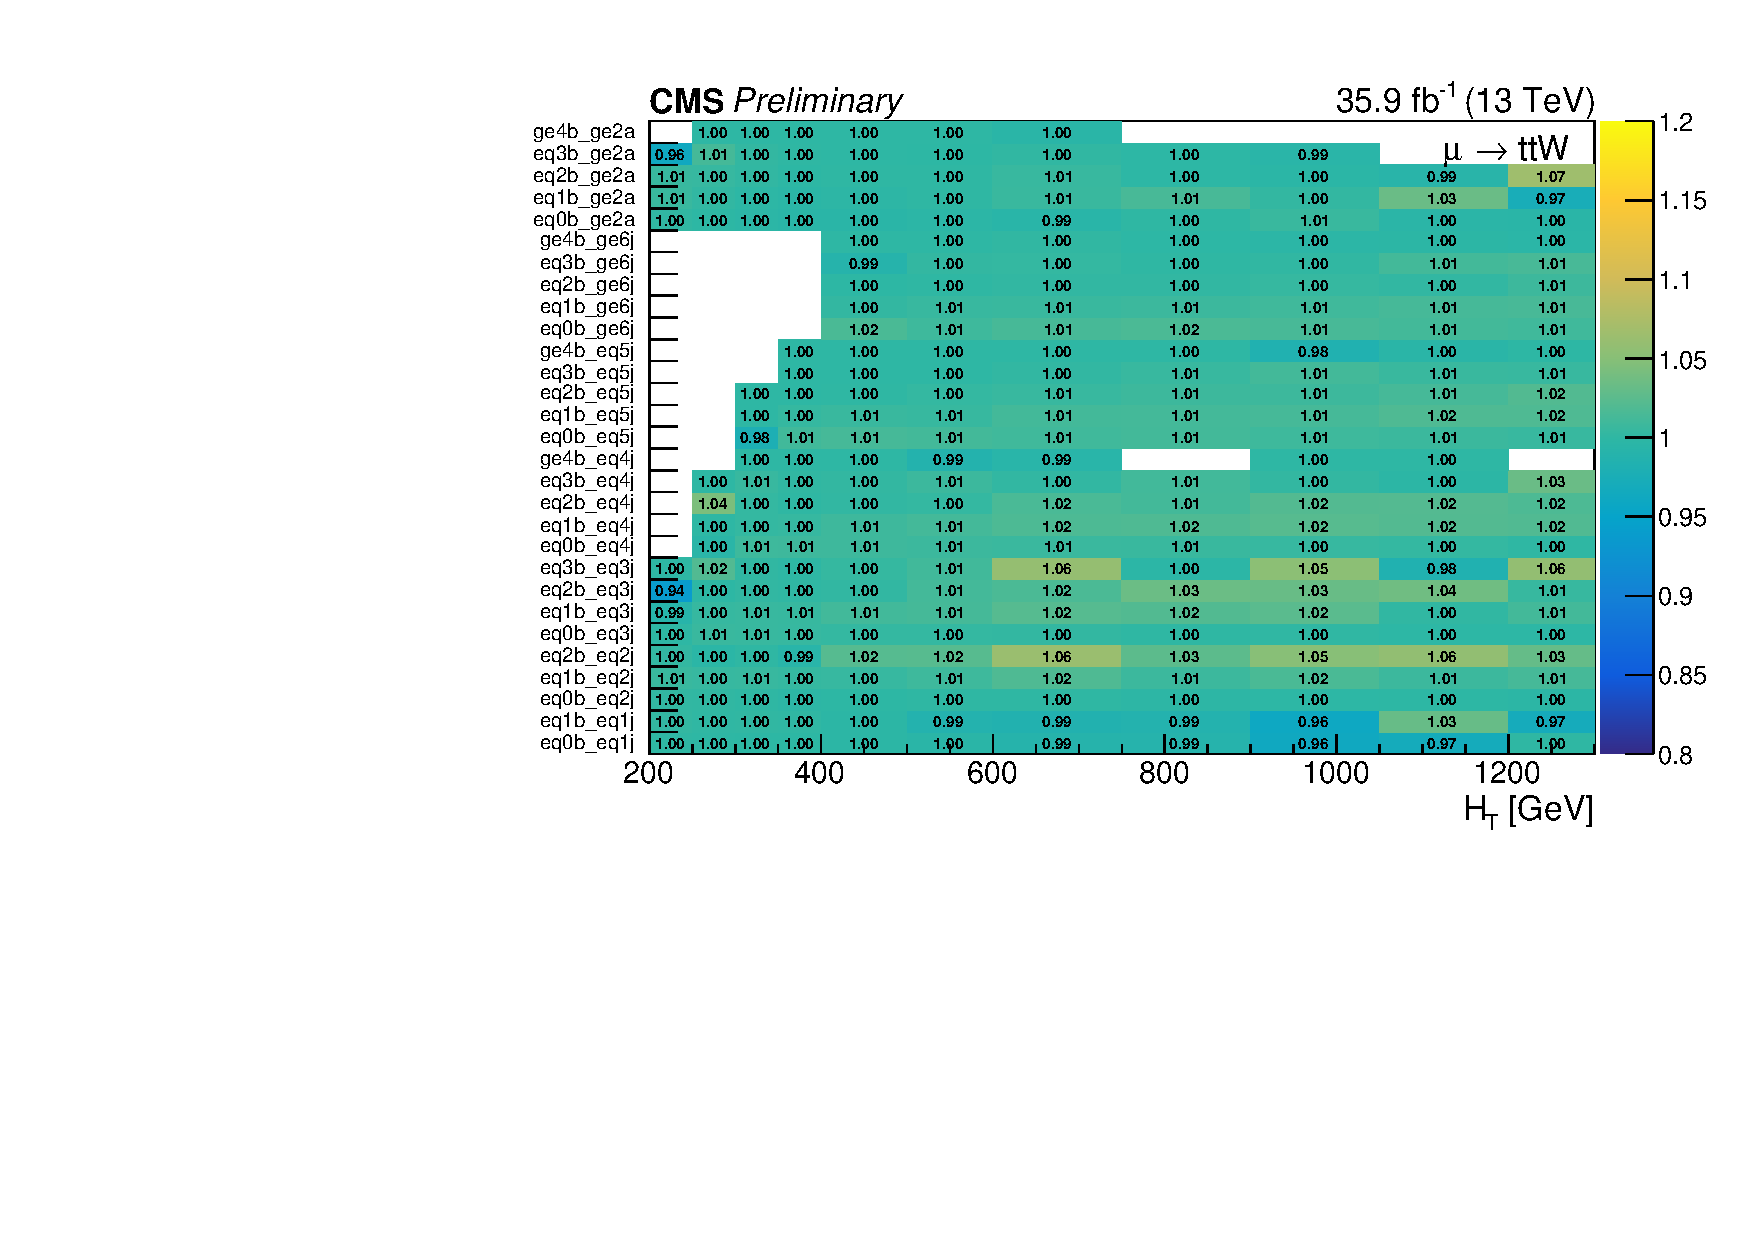
\includegraphics[width=0.5\textwidth]{figs/analysis/transferfactors/tfratio_mu_Ttw_2d_xsWeightWUp}}~
	\subfloat{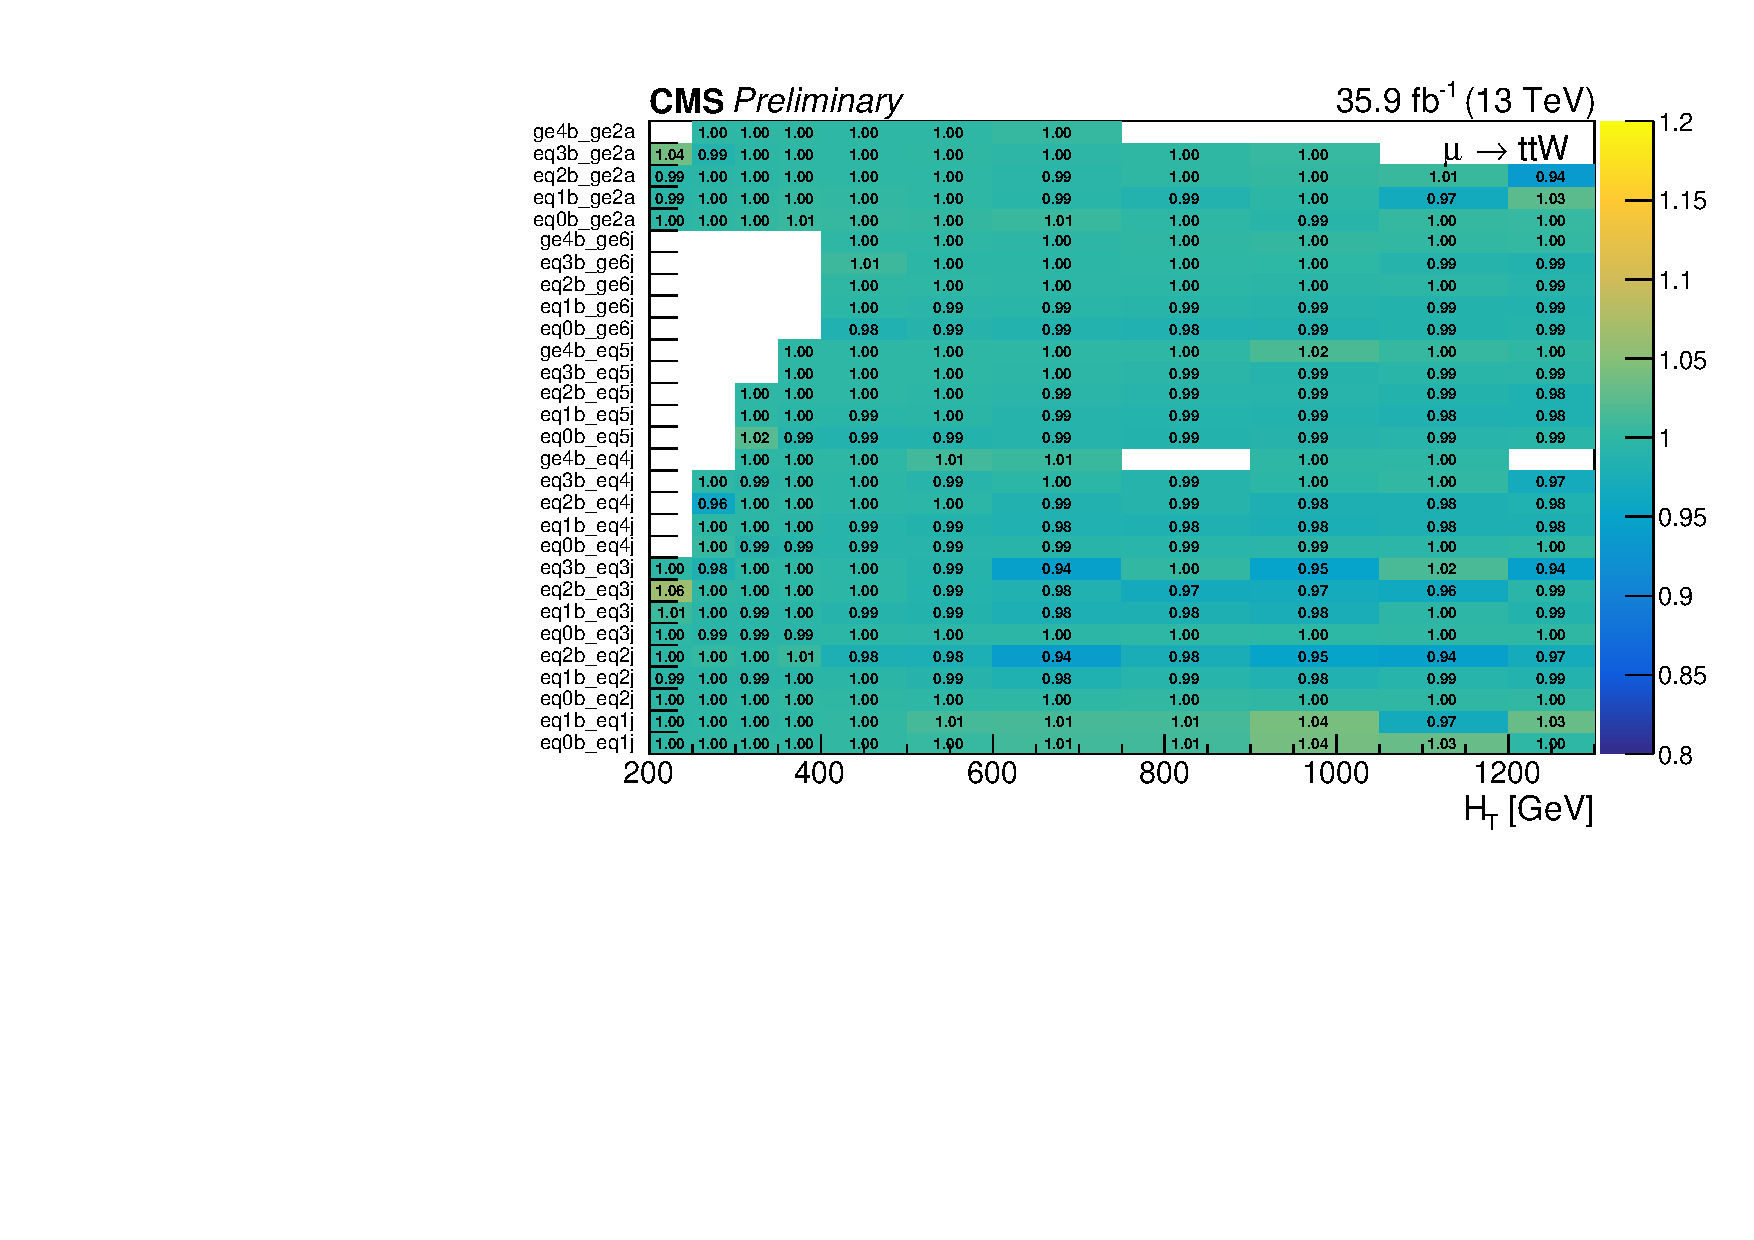
\includegraphics[width=0.5\textwidth]{figs/analysis/transferfactors/tfratio_mu_Ttw_2d_xsWeightWDown}}\\
	\subfloat{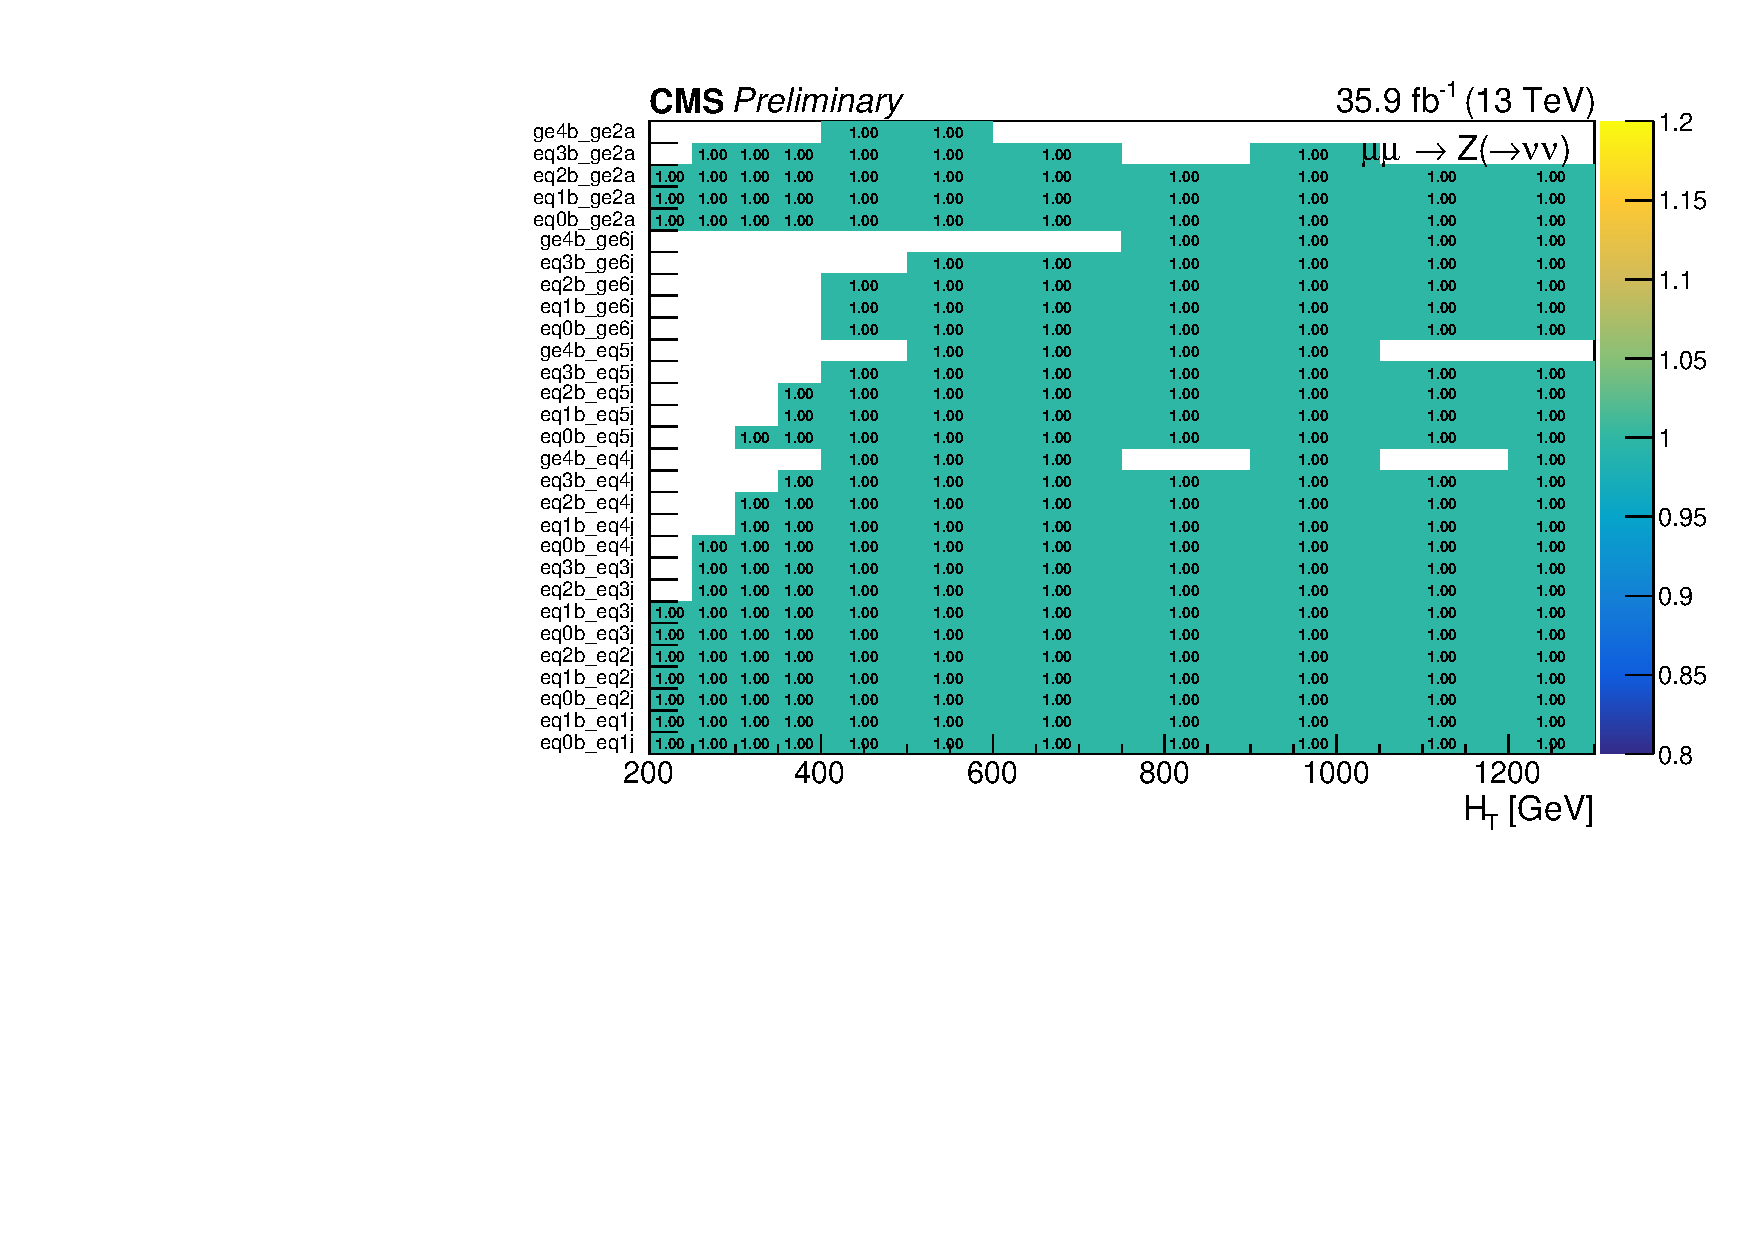
\includegraphics[width=0.5\textwidth]{figs/analysis/transferfactors/tfratio_mumu_Zinv_2d_xsWeightWUp}}~
	\subfloat{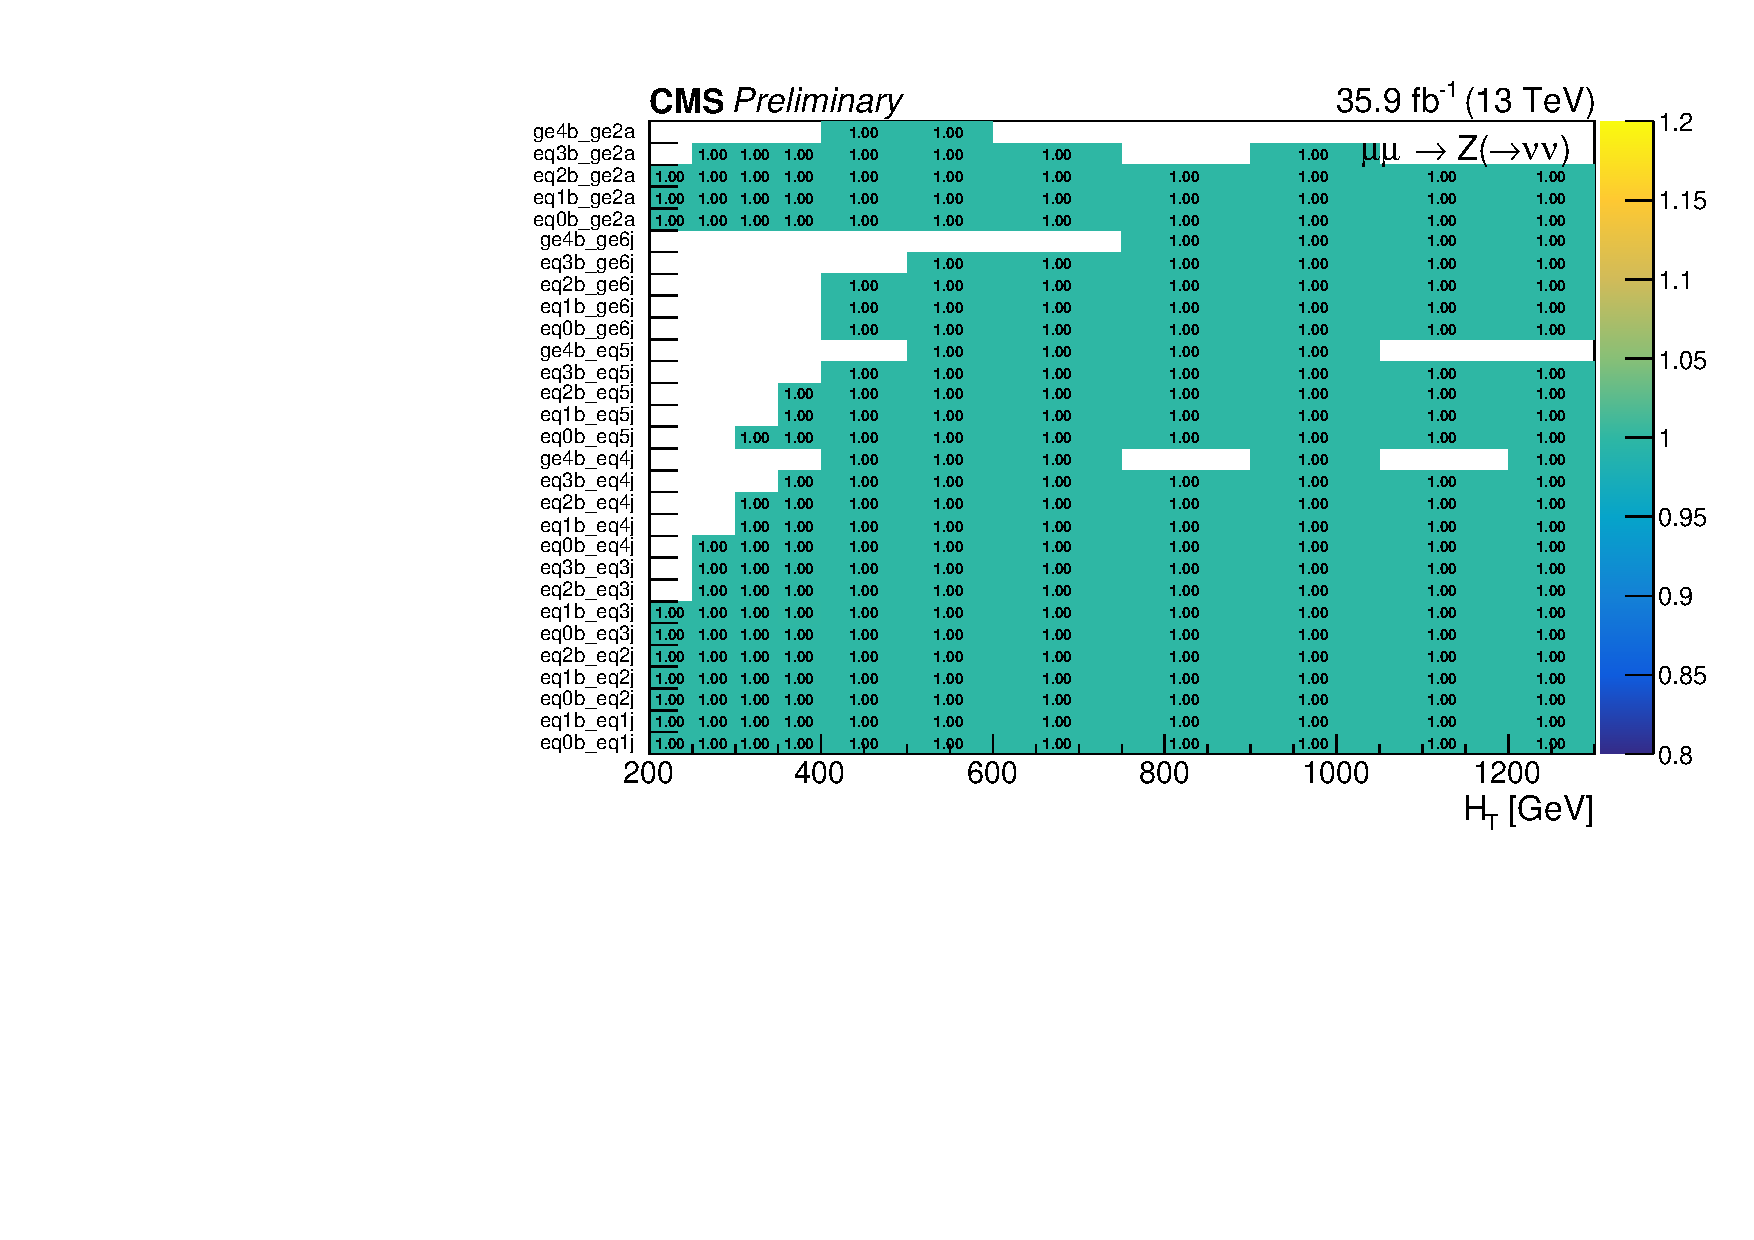
\includegraphics[width=0.5\textwidth]{figs/analysis/transferfactors/tfratio_mumu_Zinv_2d_xsWeightWDown}}\\
	\caption{The ratio of the \Tmutottw (top) and \Tmumutoz (bottom) transfer 
		factors in each \njnbht bin when varying the W cross section correction 
		factors by $+1\sigma$ (left) and $-1\sigma$ (right) with respect to 
		their nominal values.}
	\label{fig:tfvariations-xsw}
\end{figure}

\begin{figure}[h!]
	\subfloat{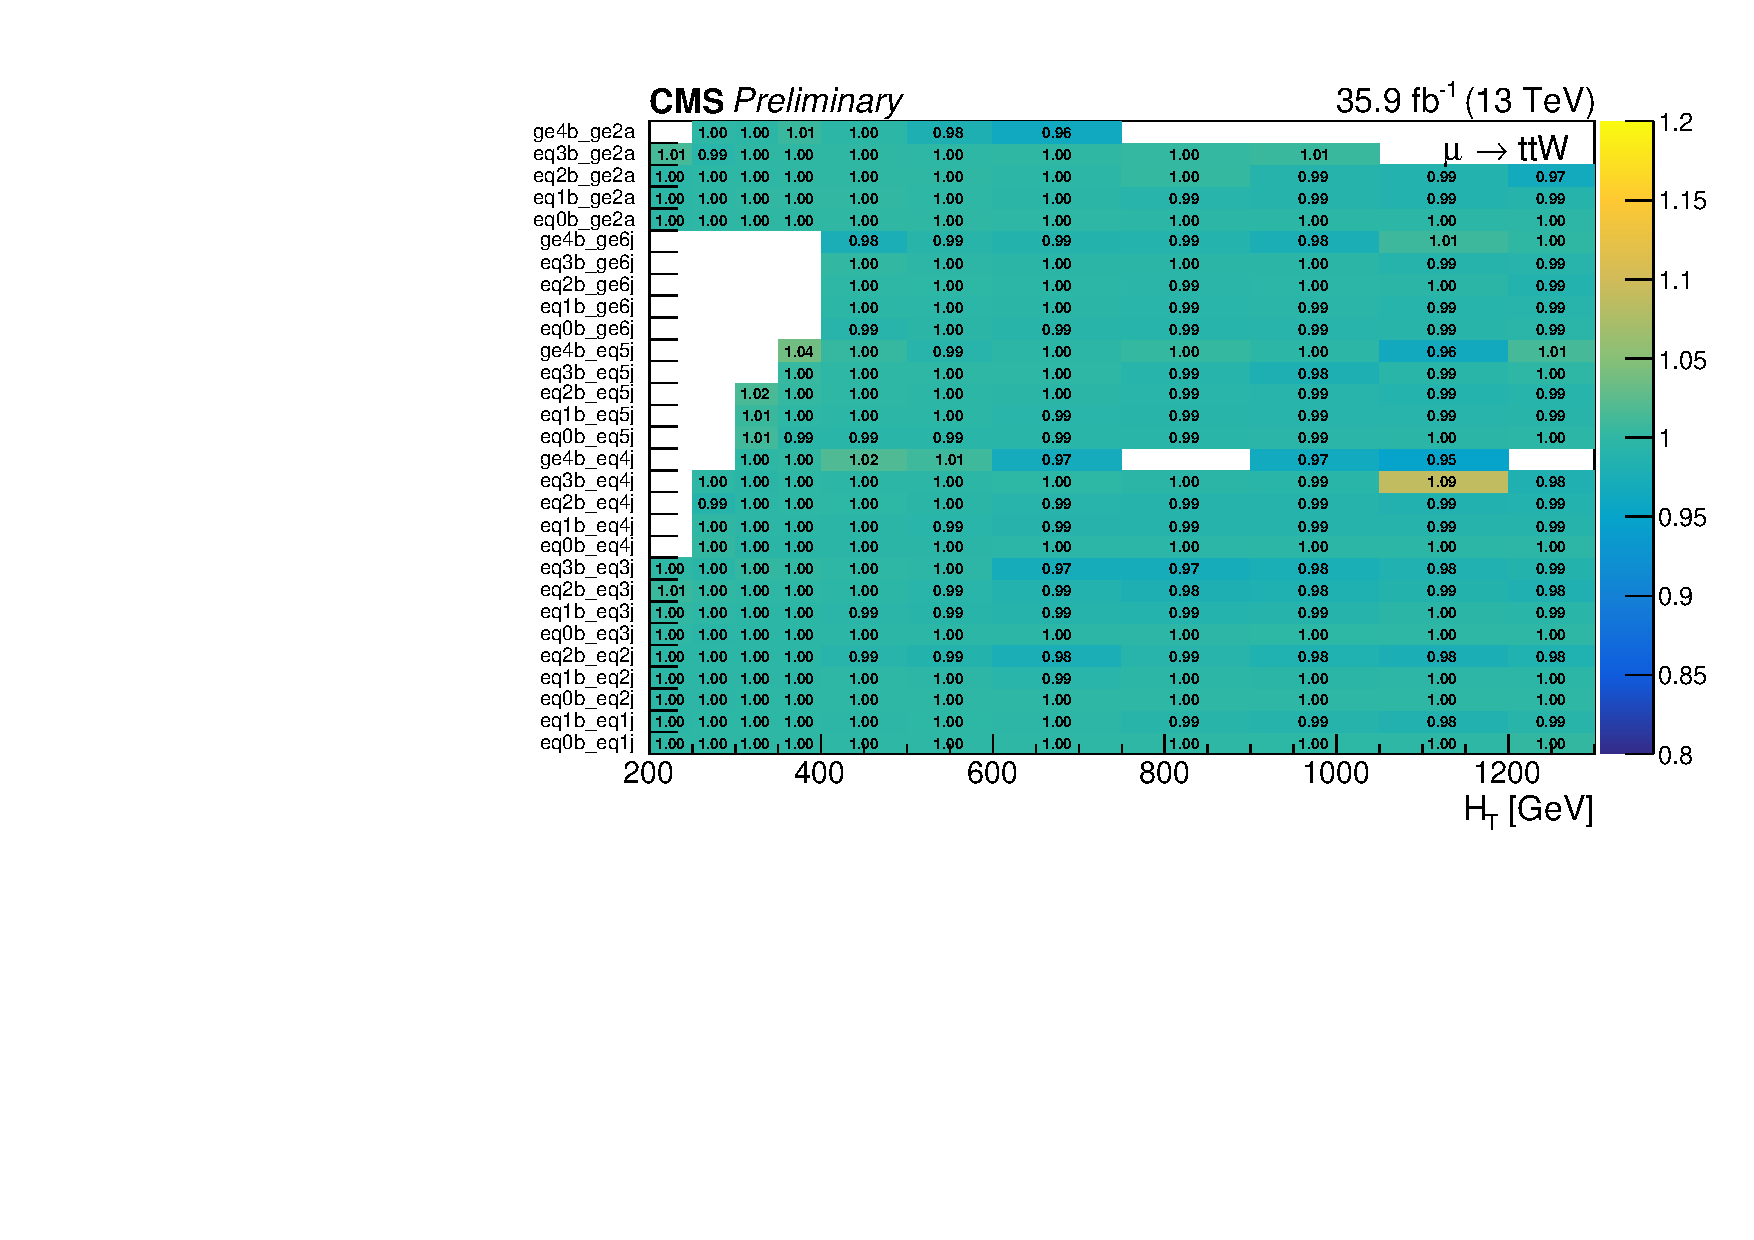
\includegraphics[width=0.5\textwidth]{figs/analysis/transferfactors/tfratio_mu_Ttw_2d_xsWeightTtUp}}~
	\subfloat{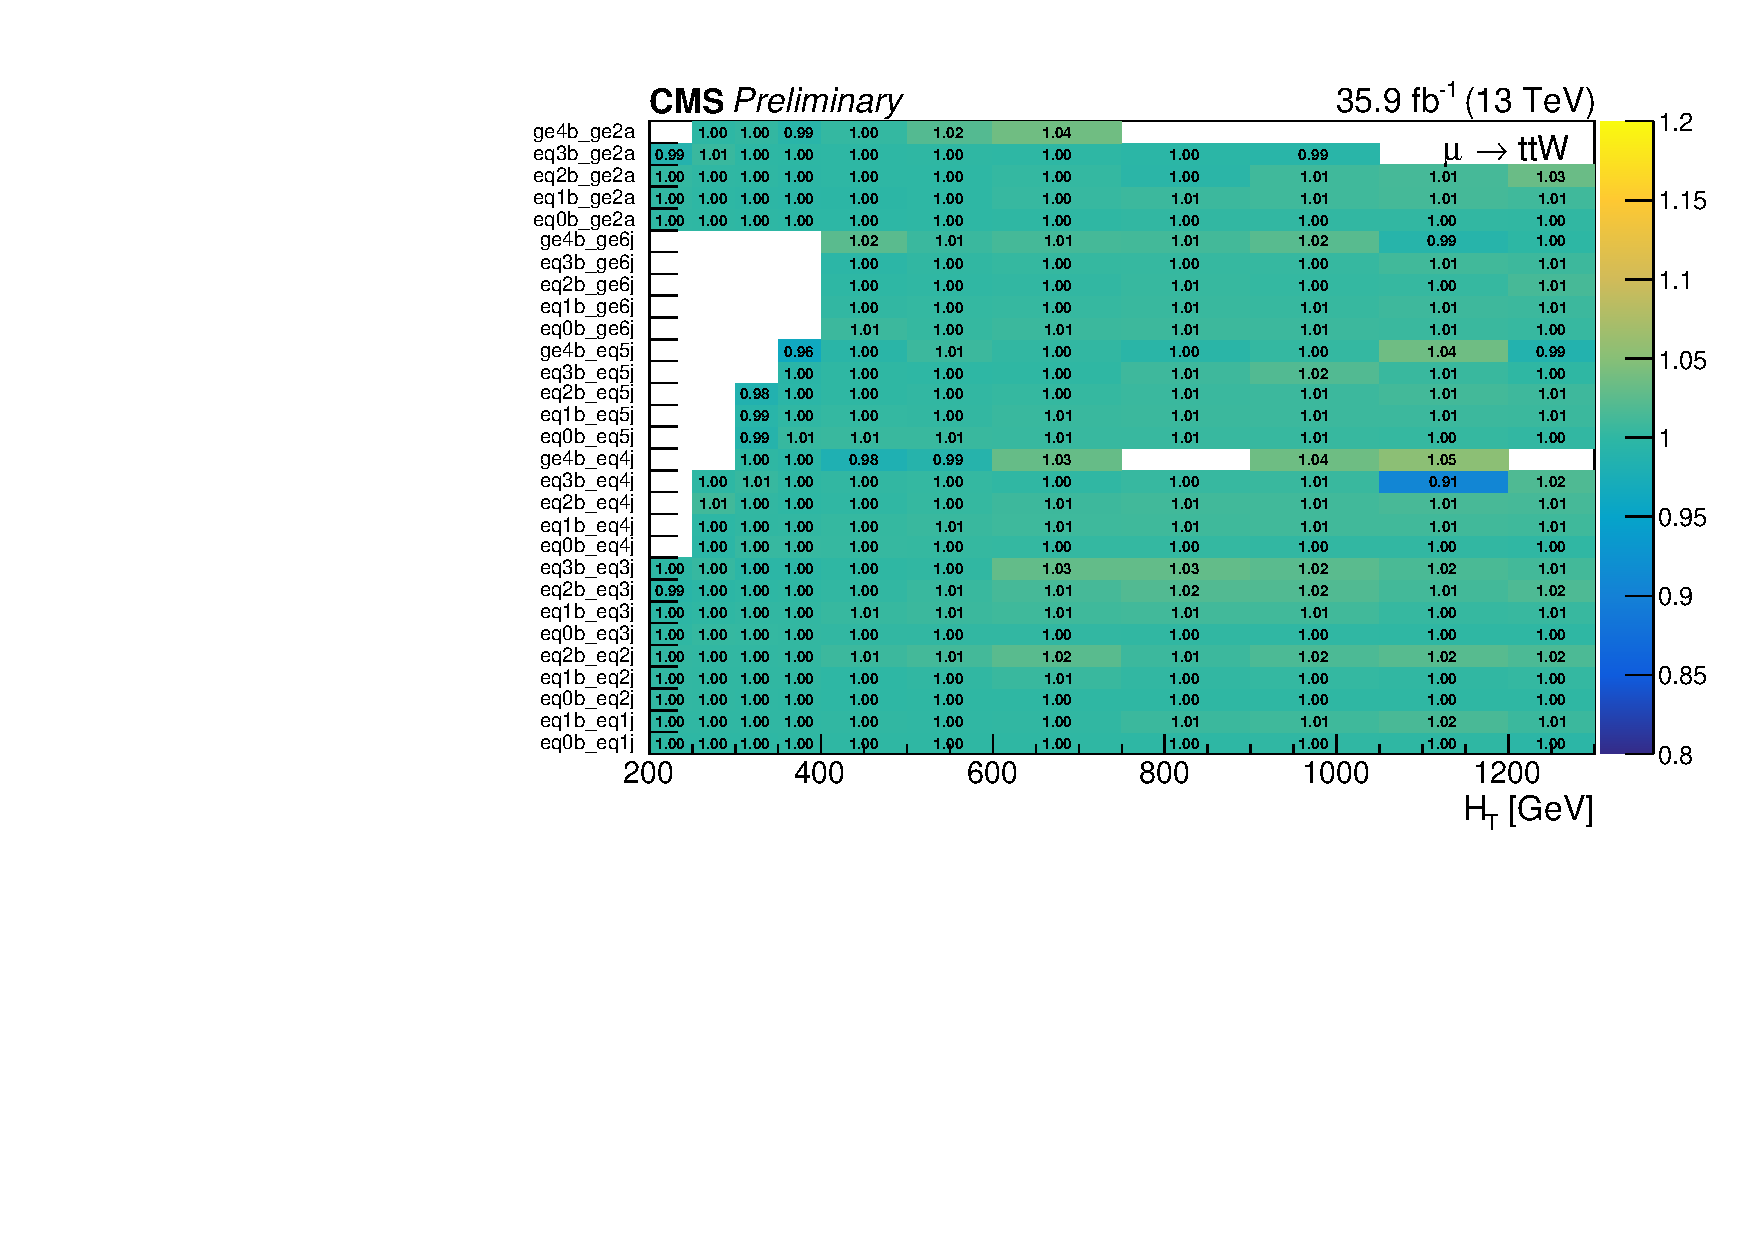
\includegraphics[width=0.5\textwidth]{figs/analysis/transferfactors/tfratio_mu_Ttw_2d_xsWeightTtDown}}\\
	\subfloat{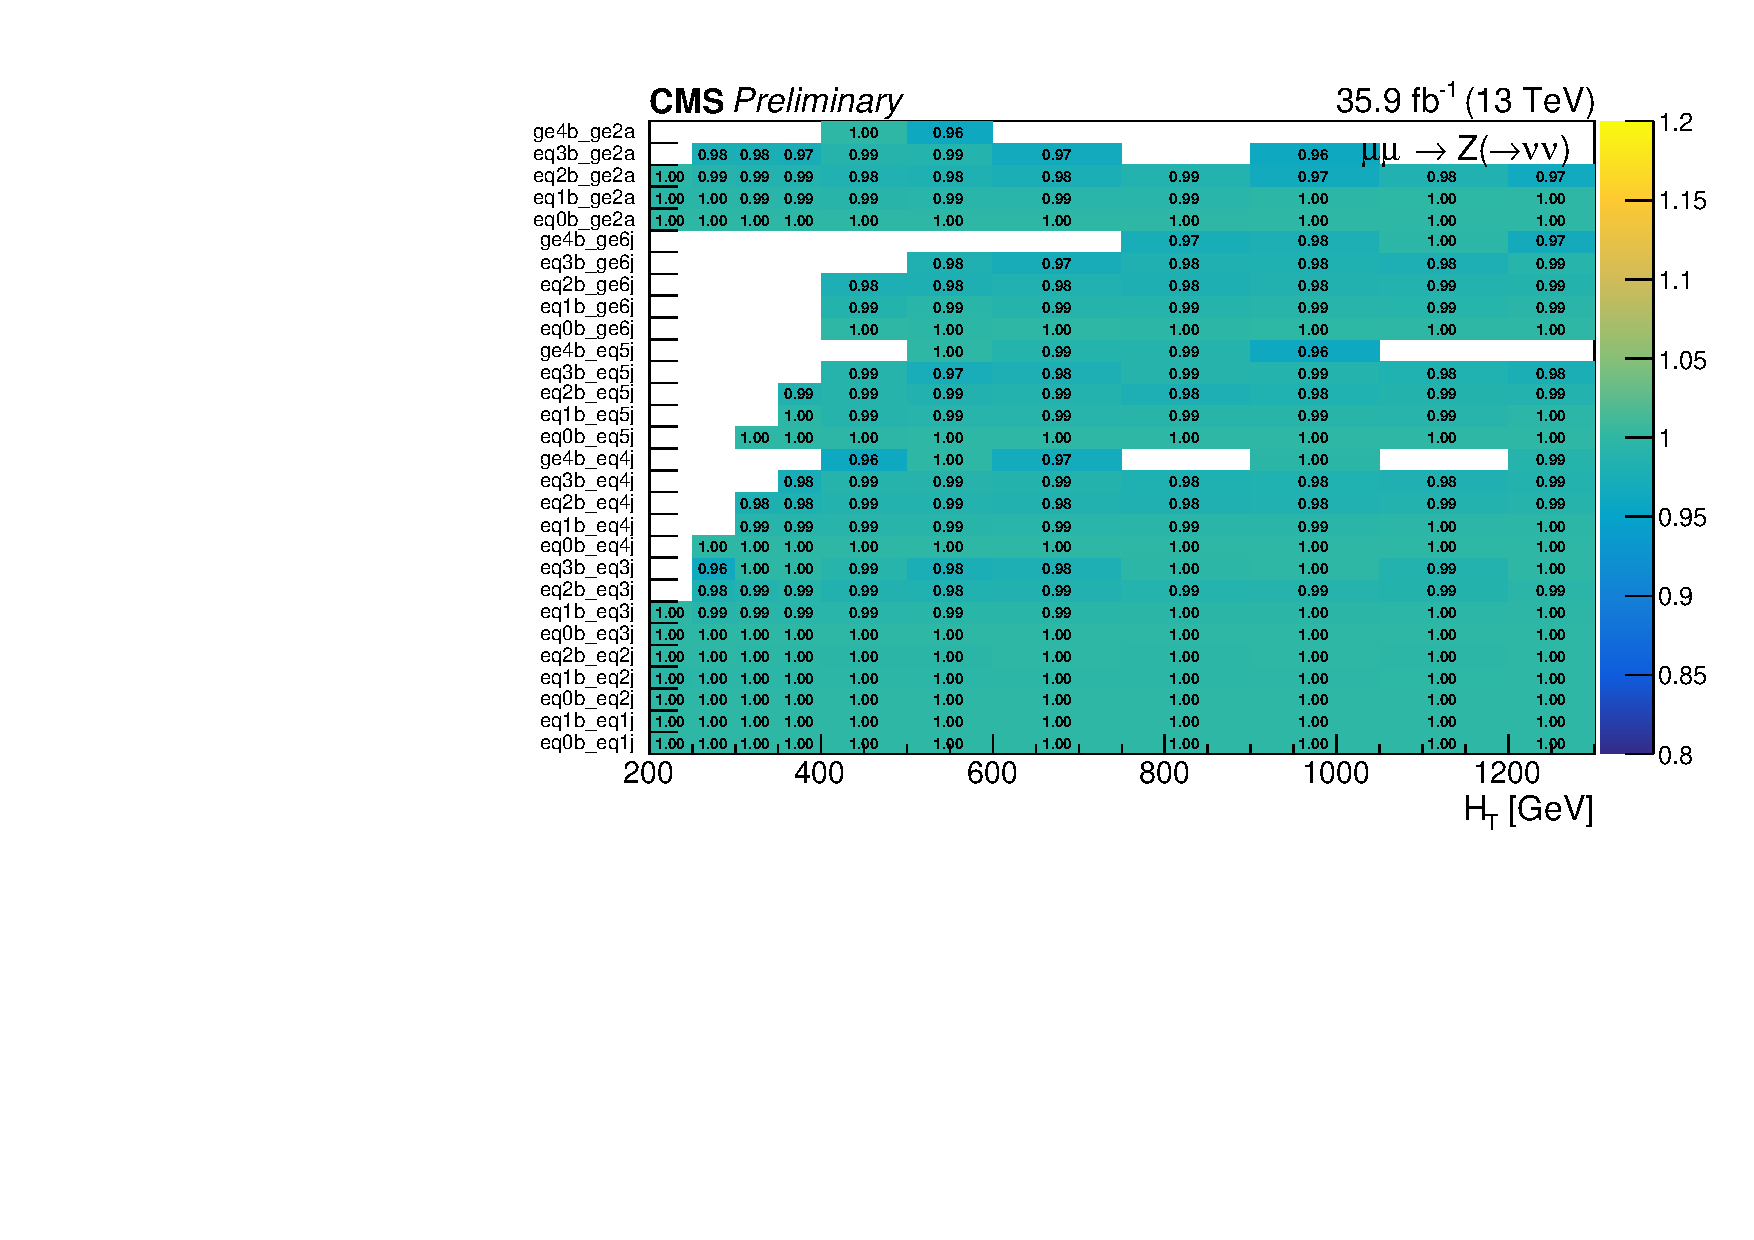
\includegraphics[width=0.5\textwidth]{figs/analysis/transferfactors/tfratio_mumu_Zinv_2d_xsWeightTtUp}}~
	\subfloat{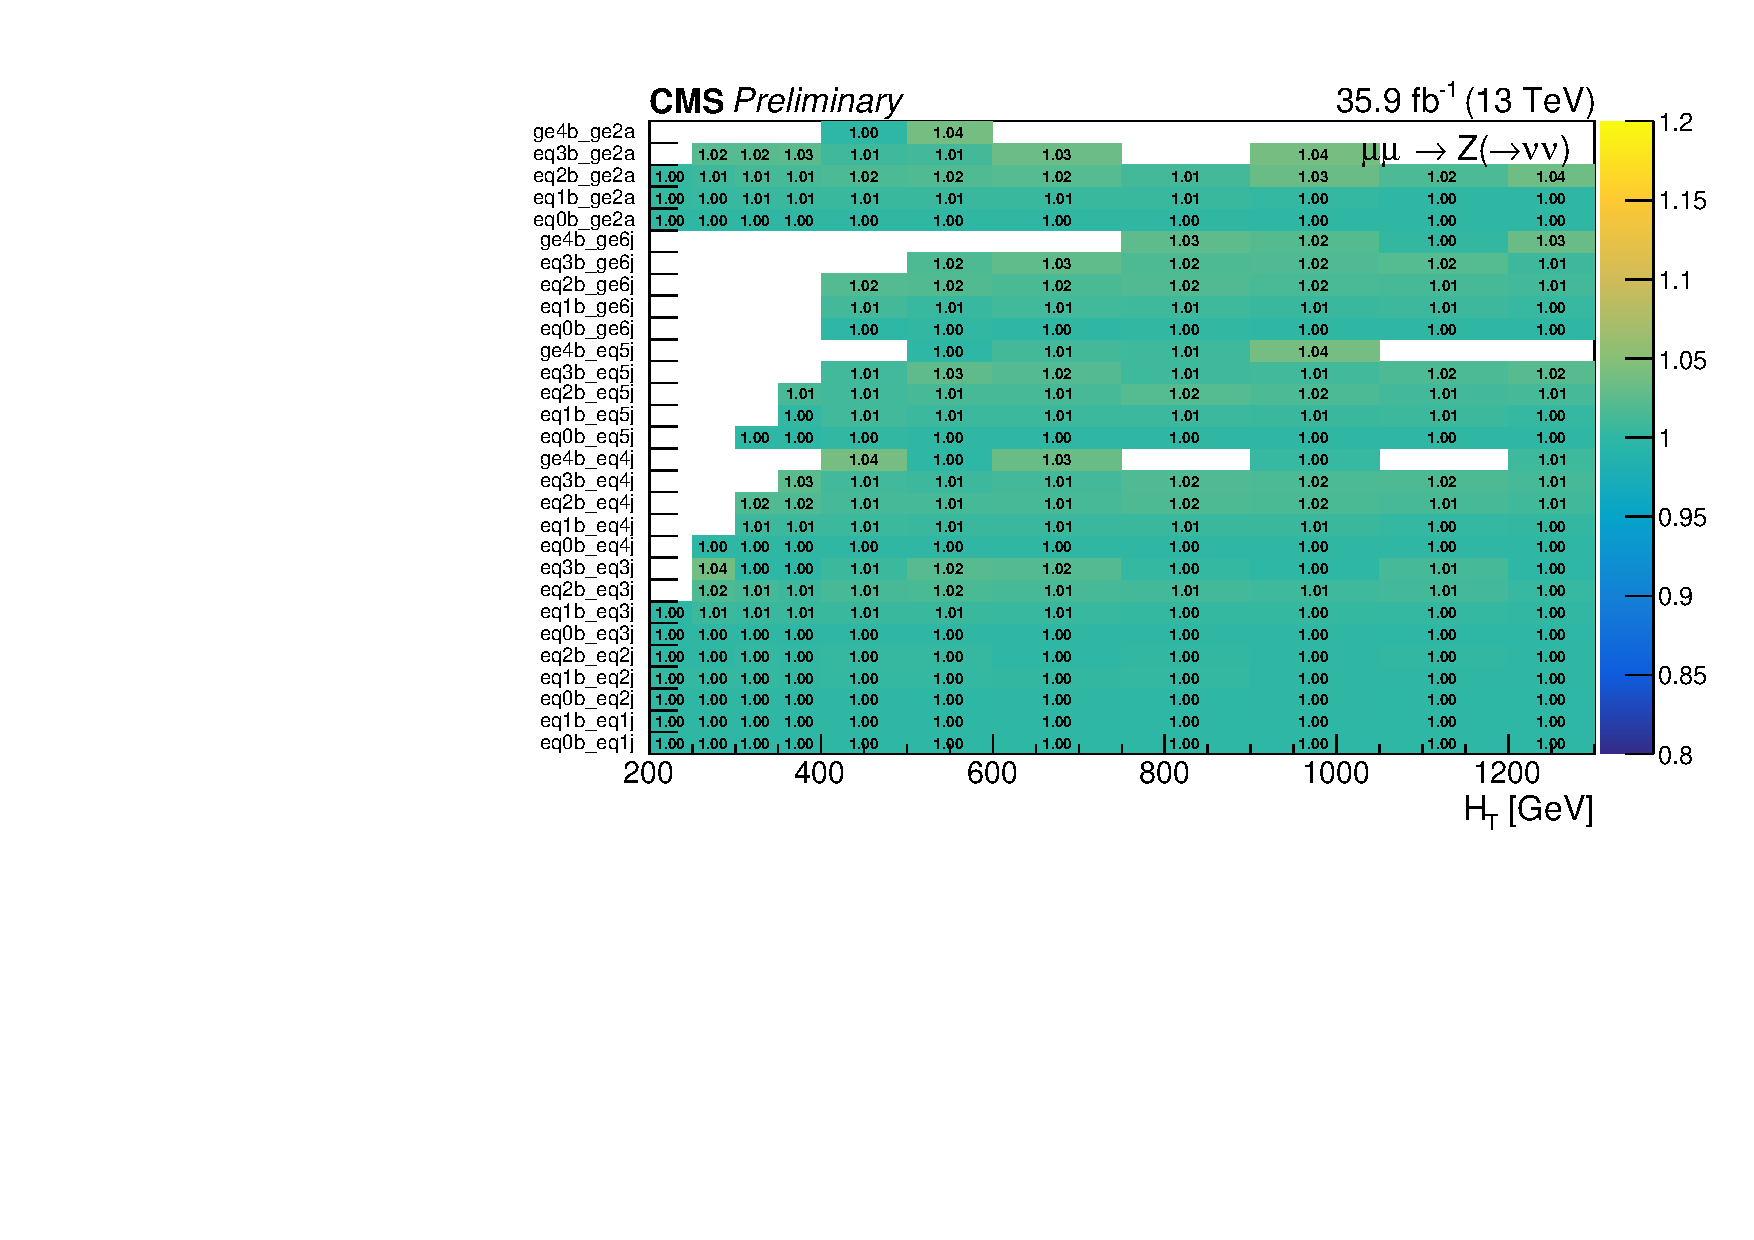
\includegraphics[width=0.5\textwidth]{figs/analysis/transferfactors/tfratio_mumu_Zinv_2d_xsWeightTtDown}}\\
	\caption{The ratio of the \Tmutottw (top) and \Tmumutoz (bottom) transfer 
		factors in each \njnbht bin when varying the \ttbar cross section 
		correction factors by $+1\sigma$ (left) and $-1\sigma$ (right) with 
		respect to 
		their nominal values.}
	\label{fig:tfvariations-xstt}
\end{figure}



\chapter{Appendix: Results and interpretation}
\label{app:results}

\section{Comparison of expected background and observed data}
\label{app:results-results}
This appendix shows the results of the maximum likelihood fit to the control 
regions under the background-only hypothesis, as discussed in 
Sec.~\ref{sec:results-results}, in tabulated form.

\clearpage
\begin{table}[!h]
	\caption{
		Observed data counts and background expectations from the 
		background-only likelihood fit to the control regions, for the 
		$\njet=1$ category. The uncertainties in the background expectations 
		include statistical as well as systematic contributions. 
	}
	\label{tab:cronly_sr_result-eq1j}
	\scriptsize
	\centering
	\begin{tabular}{rrlrrcl}
		\hline
		\njet\T\B & \nb & \scalht [GeV] & Data & \multicolumn{3}{c}{SM} \\ 
		\hline
		1\T & 0 & $ 200- 400$ & 291353 & 254856.1 &$\pm$& 30252.2 \\
		1\T & 0 & $ 400- 600$ &   8572 &   7342.2 &$\pm$&  610.4 \\
		1\T & 0 & $ 600- 900$ &    878 &    680.1 &$\pm$&  206.4 \\
		1\T & 0 & $ 900- \infty$ &     57 &     56.9 &$\pm$&   31.6 \\
		1\T & 1 & $ 200- 400$ &  11072 &   8864.3 &$\pm$& 1044.9 \\
		1\T & 1 & $ 400- 600$ &    406 &    334.6 &$\pm$&   32.4 \\
		1\T & 1 & $ 600- \infty$ &     71 &     41.5 &$\pm$&   13.1 \\
		\hline
	\end{tabular}
\end{table}

\clearpage
\begin{table}[!h]
	\caption{
		Observed data counts and background expectations from the 
		background-only likelihood fit to the control regions, for the 
		$\njet\ge2a$ category. The uncertainties in the background expectations 
		include statistical as well as systematic contributions.  
	}
	\label{tab:cronly_sr_result-ge2a}
	\scriptsize
	\centering
	\begin{tabular}{rrllrrcl}
		\hline
		\njet\T\B & \nb & \scalht [GeV] & \mht [GeV] & Data & 
		\multicolumn{3}{c}{SM} \\ 
		\hline
		$\geq 2${a}\T & 0 & $ 200- 400$ & $200-\infty$ & 116868 & 101411.4 
		&$\pm$& 14127.9 \\
		$\geq 2${a}\T & 0 & $ 400- 600$ & $200-400$ &   2932 &   2909.4 
		&$\pm$&  396.2 \\
		$\geq 2${a} & 0 & $ 400- 600$ & $400-\infty$ &   2800 &   2582.2 
		&$\pm$&  345.7 \\
		$\geq 2${a}\T & 0 & $ 600- 900$ & $200-400$ &     31 &     22.7 
		&$\pm$&    5.2 \\
		$\geq 2${a} & 0 & $ 600- 900$ & $400-600$ &     75 &     63.8 
		&$\pm$&   12.3 \\
		$\geq 2${a} & 0 & $ 600- 900$ & $600-\infty$ &    211 &    198.9 
		&$\pm$&   62.8 \\
		$\geq 2${a}\T & 0 & $ 900- \infty$ & $200-900$ &     28 &     31.8 
		&$\pm$&   12.5 \\
		$\geq 2${a} & 0 & $ 900- \infty$ & $900-\infty$ &     54 &     50.3 
		&$\pm$&   32.0 \\
		$\geq 2${a}\T & 1 & $ 200- 400$ & $200-\infty$ &  16307 &  13333.6 
		&$\pm$& 1563.7 \\
		$\geq 2${a}\T & 1 & $ 400- 600$ & $200-400$ &   1042 &    969.1 
		&$\pm$&  129.2 \\
		$\geq 2${a} & 1 & $ 400- 600$ & $400-\infty$ &    310 &    275.8 
		&$\pm$&   36.0 \\
		$\geq 2${a}\T & 1 & $ 600- 900$ & $200-400$ &      8 &     13.7 
		&$\pm$&    2.7 \\
		$\geq 2${a} & 1 & $ 600- 900$ & $400-600$ &     12 &     11.4 
		&$\pm$&    1.8 \\
		$\geq 2${a} & 1 & $ 600- 900$ & $600-\infty$ &     26 &     21.5 
		&$\pm$&    6.4 \\
		$\geq 2${a}\T & 1 & $ 900- \infty$ & $200-900$ &      5 &      3.9 
		&$\pm$&    1.5 \\
		$\geq 2${a} & 1 & $ 900- \infty$ & $900-\infty$ &      7 &      6.3 
		&$\pm$&    4.0 \\
		$\geq 2${a}\T & 2 & $ 200- 400$ & $200-\infty$ &   2200 &   1856.5 
		&$\pm$&  229.0 \\
		$\geq 2${a}\T & 2 & $ 400- 600$ & $200-400$ &    410 &    373.9 
		&$\pm$&   52.5 \\
		$\geq 2${a} & 2 & $ 400- 600$ & $400-\infty$ &     35 &     23.9 
		&$\pm$&    3.4 \\
		$\geq 2${a}\T & 2 & $ 600- 900$ & $200-400$ &      4 &      5.9 
		&$\pm$&    1.2 \\
		$\geq 2${a} & 2 & $ 600- 900$ & $400-600$ &      4 &      2.3 
		&$\pm$&    0.4 \\
		$\geq 2${a} & 2 & $ 600- 900$ & $600-\infty$ &      2 &      1.7 
		&$\pm$&    0.5 \\
		$\geq 2${a}\T & 2 & $ 900- \infty$ & $200-900$ &      1 &      0.6 
		&$\pm$&    0.1 \\
		$\geq 2${a} & 2 & $ 900- \infty$ & $900-\infty$ &      0 &      0.4 
		&$\pm$&    0.3 \\
		$\geq 2${a}\T & 3 & $ 200- 400$ & $200-\infty$ &     92 &     70.7 
		&$\pm$&   10.0 \\
		$\geq 2${a}\T & 3 & $ 400- 600$ & $200-400$ &     38 &     34.4 
		&$\pm$&    5.4 \\
		$\geq 2${a} & 3 & $ 400- 600$ & $400-\infty$ &      2 &      0.6 
		&$\pm$&    0.1 \\
		$\geq 2${a}\T & 3 & $ 600- \infty$ & $200-400$ &      1 &      0.9 
		&$\pm$&    0.2 \\
		$\geq 2${a} & 3 & $ 600- \infty$ & $400-600$ &      0 &      0.2 
		&$\pm$&    0.0 \\
		$\geq 2${a} & 3 & $ 600- \infty$ & $600-\infty$ &      0 &      0.1 
		&$\pm$&    0.0 \\
		\hline
	\end{tabular}
\end{table}

\clearpage
\begin{table}[!h]
	\caption{
		Observed data counts and background expectations from the 
		background-only likelihood fit to the control regions, for the 
		$\njet=2$ category. The uncertainties in the background expectations 
		include statistical as well as systematic contributions. 
	}
	\label{tab:cronly_sr_result-eq2j}
	\scriptsize
	\centering
	\begin{tabular}{rrllrrcl}
		\hline
		\njet\T\B & \nb & \scalht [GeV] & \mht [GeV] & Data & 
		\multicolumn{3}{c}{SM} \\ 
		\hline
		2\T & 0 & $ 200- 400$ & $200-\infty$ &  34934 &  29224.5 &$\pm$& 6798.6 
		\\
		2\T & 0 & $ 400- 600$ & $200-400$ &   3468 &   3274.3 &$\pm$&  759.7 \\
		2 & 0 & $ 400- 600$ & $400-\infty$ &   2568 &   2176.9 &$\pm$&  560.2 \\
		2\T & 0 & $ 600- 900$ & $200-400$ &    226 &    276.7 &$\pm$&   74.0 \\
		2 & 0 & $ 600- 900$ & $400-600$ &    253 &    268.4 &$\pm$&   65.1 \\
		2 & 0 & $ 600- 900$ & $600-\infty$ &    303 &    284.6 &$\pm$&  110.9 \\
		2\T & 0 & $ 900-1200$ & $200-400$ &    165 &    179.3 &$\pm$&   54.6 \\
		2 & 0 & $ 900-1200$ & $400-600$ &    125 &    130.9 &$\pm$&   34.6 \\
		2 & 0 & $ 900-1200$ & $600-900$ &     97 &     78.7 &$\pm$&   35.5 \\
		2 & 0 & $ 900-1200$ & $900-\infty$ &     25 &     29.3 &$\pm$&   19.3 \\
		2\T & 0 & $1200- \infty$ & $200-400$ &      9 &     11.8 &$\pm$&    5.1 
		\\
		2 & 0 & $1200- \infty$ & $400-600$ &     26 &     33.4 &$\pm$&    9.7 \\
		2 & 0 & $1200- \infty$ & $600-900$ &     22 &     28.0 &$\pm$&   12.9 \\
		2 & 0 & $1200- \infty$ & $900-\infty$ &     19 &     20.9 &$\pm$&   
		16.7 \\
		2\T & 1 & $ 200- 400$ & $200-\infty$ &   3850 &   3006.6 &$\pm$&  674.9 
		\\
		2\T & 1 & $ 400- 600$ & $200-400$ &    327 &    277.4 &$\pm$&   65.3 \\
		2 & 1 & $ 400- 600$ & $400-\infty$ &    240 &    219.3 &$\pm$&   55.1 \\
		2\T & 1 & $ 600- 900$ & $200-400$ &     22 &     26.9 &$\pm$&    7.1 \\
		2 & 1 & $ 600- 900$ & $400-600$ &     39 &     25.5 &$\pm$&    6.3 \\
		2 & 1 & $ 600- 900$ & $600-\infty$ &     31 &     27.1 &$\pm$&   10.1 \\
		2\T & 1 & $ 900-1200$ & $200-400$ &     17 &     19.3 &$\pm$&    5.8 \\
		2 & 1 & $ 900-1200$ & $400-600$ &     15 &     14.9 &$\pm$&    4.0 \\
		2 & 1 & $ 900-1200$ & $600-900$ &     12 &      7.4 &$\pm$&    3.3 \\
		2 & 1 & $ 900-1200$ & $900-\infty$ &      6 &      3.2 &$\pm$&    2.1 \\
		2\T & 1 & $1200- \infty$ & $200-400$ &      1 &      1.1 &$\pm$&    0.5 
		\\
		2 & 1 & $1200- \infty$ & $400-600$ &      6 &      3.4 &$\pm$&    1.0 \\
		2 & 1 & $1200- \infty$ & $600-900$ &      1 &      2.1 &$\pm$&    0.9 \\
		2 & 1 & $1200- \infty$ & $900-\infty$ &      4 &      2.0 &$\pm$&    
		1.6 \\
		2\T & 2 & $ 200- 400$ & $200-\infty$ &    254 &    196.1 &$\pm$&   44.4 
		\\
		2\T & 2 & $ 400- 600$ & $200-400$ &     22 &     13.2 &$\pm$&    3.2 \\
		2 & 2 & $ 400- 600$ & $400-\infty$ &     18 &     15.2 &$\pm$&    3.8 \\
		2\T & 2 & $ 600- \infty$ & $200-400$ &      1 &      1.8 &$\pm$&    0.5 
		\\
		2 & 2 & $ 600- \infty$ & $400-600$ &      2 &      1.9 &$\pm$&    0.5 \\
		2 & 2 & $ 600- \infty$ & $600-\infty$ &      2 &      2.3 &$\pm$&    
		0.9 \\
		\hline
	\end{tabular}
\end{table}

\clearpage
\begin{table}[!h]
	\caption{
		Observed data counts and background expectations from the 
		background-only likelihood fit to the control regions, for the 
		$\njet=3$ category. The uncertainties in the background expectations 
		include statistical as well as systematic contributions. 
	}
	\label{tab:cronly_sr_result-eq3j}
	\scriptsize
	\centering
	\begin{tabular}{rrllrrcl}
		\hline
		\njet\T\B & \nb & \scalht [GeV] & \mht [GeV] & Data & 
		\multicolumn{3}{c}{SM} \\ 
		\hline
		3\T & 0 & $ 200- 400$ & $200-\infty$ &  11815 &  10504.3 &$\pm$& 1860.3 
		\\
		3\T & 0 & $ 400- 600$ & $200-400$ &   7120 &   6666.9 &$\pm$& 1143.0 \\
		3 & 0 & $ 400- 600$ & $400-\infty$ &   1463 &   1391.0 &$\pm$&  288.2 \\
		3\T & 0 & $ 600- 900$ & $200-400$ &    668 &    698.5 &$\pm$&  132.2 \\
		3 & 0 & $ 600- 900$ & $400-600$ &    593 &    582.0 &$\pm$&  123.5 \\
		3 & 0 & $ 600- 900$ & $600-\infty$ &    246 &    231.4 &$\pm$&   91.2 \\
		3\T & 0 & $ 900-1200$ & $200-400$ &    245 &    275.3 &$\pm$&   47.6 \\
		3 & 0 & $ 900-1200$ & $400-600$ &    164 &    182.3 &$\pm$&   31.1 \\
		3 & 0 & $ 900-1200$ & $600-900$ &    101 &    109.8 &$\pm$&   42.1 \\
		3 & 0 & $ 900-1200$ & $900-\infty$ &     19 &     28.2 &$\pm$&   16.4 \\
		3\T & 0 & $1200- \infty$ & $200-400$ &     21 &     22.5 &$\pm$&    6.5 
		\\
		3 & 0 & $1200- \infty$ & $400-600$ &     28 &     54.2 &$\pm$&   11.0 \\
		3 & 0 & $1200- \infty$ & $600-900$ &     31 &     36.1 &$\pm$&   13.3 \\
		3 & 0 & $1200- \infty$ & $900-\infty$ &     17 &     22.0 &$\pm$&   
		15.6 \\
		3\T & 1 & $ 200- 400$ & $200-\infty$ &   2703 &   2242.6 &$\pm$&  400.0 
		\\
		3\T & 1 & $ 400- 600$ & $200-400$ &   1212 &   1125.8 &$\pm$&  197.2 \\
		3 & 1 & $ 400- 600$ & $400-\infty$ &    301 &    222.4 &$\pm$&   42.5 \\
		3\T & 1 & $ 600- 900$ & $200-400$ &    110 &     94.6 &$\pm$&   18.3 \\
		3 & 1 & $ 600- 900$ & $400-600$ &     96 &     77.9 &$\pm$&   16.2 \\
		3 & 1 & $ 600- 900$ & $600-\infty$ &     42 &     32.7 &$\pm$&   12.4 \\
		3\T & 1 & $ 900-1200$ & $200-400$ &     39 &     41.2 &$\pm$&    7.5 \\
		3 & 1 & $ 900-1200$ & $400-600$ &     24 &     23.9 &$\pm$&    4.1 \\
		3 & 1 & $ 900-1200$ & $600-900$ &     10 &     15.4 &$\pm$&    5.8 \\
		3 & 1 & $ 900-1200$ & $900-\infty$ &      6 &      4.4 &$\pm$&    2.2 \\
		3\T & 1 & $1200- \infty$ & $200-400$ &      3 &      3.4 &$\pm$&    0.9 
		\\
		3 & 1 & $1200- \infty$ & $400-600$ &      5 &      7.5 &$\pm$&    1.6 \\
		3 & 1 & $1200- \infty$ & $600-900$ &      7 &      5.1 &$\pm$&    1.9 \\
		3 & 1 & $1200- \infty$ & $900-\infty$ &      4 &      3.5 &$\pm$&    
		2.4 \\
		3\T & 2 & $ 200- 400$ & $200-\infty$ &    495 &    418.2 &$\pm$&   79.0 
		\\
		3\T & 2 & $ 400- 600$ & $200-400$ &    229 &    208.3 &$\pm$&   38.9 \\
		3 & 2 & $ 400- 600$ & $400-\infty$ &     34 &     27.0 &$\pm$&    5.2 \\
		3\T & 2 & $ 600- 900$ & $200-400$ &     10 &      9.1 &$\pm$&    1.8 \\
		3 & 2 & $ 600- 900$ & $400-600$ &      9 &      9.3 &$\pm$&    1.9 \\
		3 & 2 & $ 600- 900$ & $600-\infty$ &      2 &      3.2 &$\pm$&    1.2 \\
		3\T & 2 & $ 900-1200$ & $200-400$ &      4 &      3.5 &$\pm$&    0.7 \\
		3 & 2 & $ 900-1200$ & $400-600$ &      2 &      1.8 &$\pm$&    0.3 \\
		3 & 2 & $ 900-1200$ & $600-900$ &      2 &      1.3 &$\pm$&    0.5 \\
		3 & 2 & $ 900-1200$ & $900-\infty$ &      0 &      0.4 &$\pm$&    0.2 \\
		3\T & 2 & $1200- \infty$ & $200-400$ &      1 &      0.3 &$\pm$&    0.1 
		\\
		3 & 2 & $1200- \infty$ & $400-600$ &      0 &      0.7 &$\pm$&    0.1 \\
		3 & 2 & $1200- \infty$ & $600-900$ &      0 &      0.4 &$\pm$&    0.2 \\
		3 & 2 & $1200- \infty$ & $900-\infty$ &      0 &      0.3 &$\pm$&    
		0.2 \\
		3\T & 3 & $ 200- 400$ & $200-\infty$ &     16 &     12.1 &$\pm$&    2.5 
		\\
		3\T & 3 & $ 400- 600$ & $200-400$ &     10 &      7.9 &$\pm$&    1.6 \\
		3 & 3 & $ 400- 600$ & $400-\infty$ &      2 &      0.8 &$\pm$&    0.2 \\
		3\T & 3 & $ 600- \infty$ & $200-400$ &      3 &      0.4 &$\pm$&    0.1 
		\\
		3 & 3 & $ 600- \infty$ & $400-600$ &      3 &      0.3 &$\pm$&    0.1 \\
		3 & 3 & $ 600- \infty$ & $600-\infty$ &      0 &      0.2 &$\pm$&    
		0.1 \\
		\hline
	\end{tabular}
\end{table}

\clearpage
\begin{table}[!h]
	\caption{
		Observed data counts and background expectations from the 
		background-only likelihood fit to the control regions, for the 
		$\njet=4$ category. The uncertainties in the background expectations 
		include statistical as well as systematic contributions. 
	}
	\label{tab:cronly_sr_result-eq4j}
	\scriptsize
	\centering
	\begin{tabular}{rrllrrcl}
		\hline
		\njet\T\B & \nb & \scalht [GeV] & \mht [GeV] & Data & 
		\multicolumn{3}{c}{SM} \\ 
		\hline
		4\T & 0 & $ 400- 600$ & $200-400$ &   4324 &   4749.1 &$\pm$&  621.7 \\
		4 & 0 & $ 400- 600$ & $400-\infty$ &    437 &    460.4 &$\pm$&   78.3 \\
		4\T & 0 & $ 600- 900$ & $200-400$ &    751 &    937.0 &$\pm$&  113.5 \\
		4 & 0 & $ 600- 900$ & $400-600$ &    484 &    521.7 &$\pm$&   76.4 \\
		4 & 0 & $ 600- 900$ & $600-\infty$ &    110 &    103.7 &$\pm$&   35.1 \\
		4\T & 0 & $ 900-1200$ & $200-400$ &    186 &    251.2 &$\pm$&   36.7 \\
		4 & 0 & $ 900-1200$ & $400-600$ &    111 &    142.9 &$\pm$&   20.7 \\
		4 & 0 & $ 900-1200$ & $600-900$ &     66 &     71.7 &$\pm$&   25.6 \\
		4 & 0 & $ 900-1200$ & $900-\infty$ &     13 &     10.6 &$\pm$&    5.8 \\
		4\T & 0 & $1200- \infty$ & $200-400$ &     13 &     23.8 &$\pm$&    6.0 
		\\
		4 & 0 & $1200- \infty$ & $400-600$ &     32 &     43.0 &$\pm$&    8.2 \\
		4 & 0 & $1200- \infty$ & $600-900$ &     28 &     26.8 &$\pm$&    9.9 \\
		4 & 0 & $1200- \infty$ & $900-\infty$ &     15 &     13.9 &$\pm$&    
		9.4 \\
		4\T & 1 & $ 400- 600$ & $200-400$ &   1497 &   1444.4 &$\pm$&  191.1 \\
		4 & 1 & $ 400- 600$ & $400-\infty$ &    109 &    109.8 &$\pm$&   16.5 \\
		4\T & 1 & $ 600- 900$ & $200-400$ &    184 &    196.6 &$\pm$&   23.6 \\
		4 & 1 & $ 600- 900$ & $400-600$ &    106 &    100.9 &$\pm$&   14.0 \\
		4 & 1 & $ 600- 900$ & $600-\infty$ &     19 &     17.2 &$\pm$&    5.5 \\
		4\T & 1 & $ 900-1200$ & $200-400$ &     60 &     53.8 &$\pm$&    7.6 \\
		4 & 1 & $ 900-1200$ & $400-600$ &     19 &     27.7 &$\pm$&    4.1 \\
		4 & 1 & $ 900-1200$ & $600-900$ &     11 &     12.3 &$\pm$&    4.2 \\
		4 & 1 & $ 900-1200$ & $900-\infty$ &      1 &      1.8 &$\pm$&    1.0 \\
		4\T & 1 & $1200- \infty$ & $200-400$ &      7 &      5.2 &$\pm$&    1.3 
		\\
		4 & 1 & $1200- \infty$ & $400-600$ &     11 &     10.6 &$\pm$&    2.1 \\
		4 & 1 & $1200- \infty$ & $600-900$ &      7 &      4.8 &$\pm$&    1.7 \\
		4 & 1 & $1200- \infty$ & $900-\infty$ &      4 &      2.9 &$\pm$&    
		1.8 \\
		4\T & 2 & $ 400- 600$ & $200-400$ &    524 &    490.0 &$\pm$&   72.7 \\
		4 & 2 & $ 400- 600$ & $400-\infty$ &     29 &     24.0 &$\pm$&    4.0 \\
		4\T & 2 & $ 600- 900$ & $200-400$ &     50 &     39.2 &$\pm$&    5.0 \\
		4 & 2 & $ 600- 900$ & $400-600$ &     19 &     19.9 &$\pm$&    2.7 \\
		4 & 2 & $ 600- 900$ & $600-\infty$ &      1 &      2.4 &$\pm$&    0.7 \\
		4\T & 2 & $ 900-1200$ & $200-400$ &     10 &      8.7 &$\pm$&    1.2 \\
		4 & 2 & $ 900-1200$ & $400-600$ &      7 &      4.1 &$\pm$&    0.7 \\
		4 & 2 & $ 900-1200$ & $600-900$ &      0 &      1.7 &$\pm$&    0.6 \\
		4 & 2 & $ 900-1200$ & $900-\infty$ &      1 &      0.3 &$\pm$&    0.2 \\
		4\T & 2 & $1200- \infty$ & $200-400$ &      1 &      0.7 &$\pm$&    0.2 
		\\
		4 & 2 & $1200- \infty$ & $400-600$ &      0 &      1.5 &$\pm$&    0.3 \\
		4 & 2 & $1200- \infty$ & $600-900$ &      0 &      0.5 &$\pm$&    0.2 \\
		4 & 2 & $1200- \infty$ & $900-\infty$ &      1 &      0.4 &$\pm$&    
		0.2 \\
		4\T & 3 & $ 400- 600$ & $200-400$ &     35 &     36.8 &$\pm$&    6.0 \\
		4 & 3 & $ 400- 600$ & $400-\infty$ &      1 &      1.6 &$\pm$&    0.3 \\
		4\T & 3 & $ 600- 900$ & $200-400$ &      6 &      2.5 &$\pm$&    0.3 \\
		4 & 3 & $ 600- 900$ & $400-600$ &      0 &      1.2 &$\pm$&    0.2 \\
		4 & 3 & $ 600- 900$ & $600-\infty$ &      0 &      0.2 &$\pm$&    0.0 \\
		4\T & 3 & $ 900- \infty$ & $200-400$ &      0 &      0.7 &$\pm$&    0.1 
		\\
		4 & 3 & $ 900- \infty$ & $400-600$ &      0 &      0.4 &$\pm$&    0.1 \\
		4 & 3 & $ 900- \infty$ & $600-900$ &      0 &      0.1 &$\pm$&    0.0 \\
		4 & 3 & $ 900- \infty$ & $900-\infty$ &      0 &      0.0 &$\pm$&    
		0.0 \\
		\hline
	\end{tabular}
\end{table}

\clearpage
\begin{table}[!h]
	\caption{
		Observed data counts and background expectations from the 
		background-only likelihood fit to the control regions, for the 
		$\njet=5$ category. The uncertainties in the background expectations 
		include statistical as well as systematic contributions. 
	}
	\label{tab:cronly_sr_result-eq5j}
	\scriptsize
	\centering
	\begin{tabular}{rrllrrcl}
		\hline
		\njet\T\B & \nb & \scalht [GeV] & \mht [GeV] & Data & 
		\multicolumn{3}{c}{SM} \\ 
		\hline
		5\T & 0 & $ 400- 600$ & $200-400$ &   1132 &   1250.0 &$\pm$&  197.6 \\
		5 & 0 & $ 400- 600$ & $400-\infty$ &     59 &     74.0 &$\pm$&   16.6 \\
		5\T & 0 & $ 600- 900$ & $200-400$ &    435 &    561.4 &$\pm$&   80.0 \\
		5 & 0 & $ 600- 900$ & $400-600$ &    201 &    197.5 &$\pm$&   35.4 \\
		5 & 0 & $ 600- 900$ & $600-\infty$ &     17 &     25.9 &$\pm$&    9.5 \\
		5\T & 0 & $ 900-1200$ & $200-400$ &    124 &    149.9 &$\pm$&   21.2 \\
		5 & 0 & $ 900-1200$ & $400-600$ &     59 &     68.1 &$\pm$&   10.1 \\
		5 & 0 & $ 900-1200$ & $600-\infty$ &     28 &     30.7 &$\pm$&   11.6 \\
		5\T & 0 & $1200- \infty$ & $200-400$ &      7 &     18.1 &$\pm$&    4.7 
		\\
		5 & 0 & $1200- \infty$ & $400-600$ &     16 &     23.1 &$\pm$&    4.7 \\
		5 & 0 & $1200- \infty$ & $600-900$ &      7 &     13.2 &$\pm$&    5.2 \\
		5 & 0 & $1200- \infty$ & $900-\infty$ &      6 &      6.2 &$\pm$&    
		4.3 \\
		5\T & 1 & $ 400- 600$ & $200-400$ &    591 &    608.6 &$\pm$&  105.2 \\
		5 & 1 & $ 400- 600$ & $400-\infty$ &     22 &     22.0 &$\pm$&    4.5 \\
		5\T & 1 & $ 600- 900$ & $200-400$ &    198 &    194.1 &$\pm$&   29.9 \\
		5 & 1 & $ 600- 900$ & $400-600$ &     50 &     55.2 &$\pm$&    9.2 \\
		5 & 1 & $ 600- 900$ & $600-\infty$ &     11 &      5.9 &$\pm$&    1.9 \\
		5\T & 1 & $ 900-1200$ & $200-400$ &     33 &     41.0 &$\pm$&    5.8 \\
		5 & 1 & $ 900-1200$ & $400-600$ &     15 &     16.9 &$\pm$&    2.4 \\
		5 & 1 & $ 900-1200$ & $600-\infty$ &      9 &      7.0 &$\pm$&    2.4 \\
		5\T & 1 & $1200- \infty$ & $200-400$ &      4 &      4.5 &$\pm$&    1.1 
		\\
		5 & 1 & $1200- \infty$ & $400-600$ &      3 &      6.1 &$\pm$&    1.2 \\
		5 & 1 & $1200- \infty$ & $600-900$ &      5 &      2.8 &$\pm$&    1.0 \\
		5 & 1 & $1200- \infty$ & $900-\infty$ &      2 &      1.6 &$\pm$&    
		1.1 \\
		5\T & 2 & $ 400- 600$ & $200-400$ &    284 &    273.9 &$\pm$&   51.3 \\
		5 & 2 & $ 400- 600$ & $400-\infty$ &     10 &      4.8 &$\pm$&    1.0 \\
		5\T & 2 & $ 600- 900$ & $200-400$ &     63 &     67.5 &$\pm$&   11.6 \\
		5 & 2 & $ 600- 900$ & $400-600$ &     16 &     16.5 &$\pm$&    2.8 \\
		5 & 2 & $ 600- 900$ & $600-\infty$ &      0 &      1.3 &$\pm$&    0.4 \\
		5\T & 2 & $ 900-1200$ & $200-400$ &      5 &     10.5 &$\pm$&    1.6 \\
		5 & 2 & $ 900-1200$ & $400-600$ &      5 &      3.5 &$\pm$&    0.6 \\
		5 & 2 & $ 900-1200$ & $600-\infty$ &      1 &      1.5 &$\pm$&    0.5 \\
		5\T & 2 & $1200- \infty$ & $200-400$ &      0 &      1.0 &$\pm$&    0.2 
		\\
		5 & 2 & $1200- \infty$ & $400-600$ &      2 &      1.2 &$\pm$&    0.2 \\
		5 & 2 & $1200- \infty$ & $600-900$ &      1 &      0.4 &$\pm$&    0.1 \\
		5 & 2 & $1200- \infty$ & $900-\infty$ &      1 &      0.3 &$\pm$&    
		0.2 \\
		5\T & 3 & $ 400- 600$ & $200-400$ &     25 &     28.0 &$\pm$&    5.4 \\
		5 & 3 & $ 400- 600$ & $400-\infty$ &      1 &      0.3 &$\pm$&    0.1 \\
		5\T & 3 & $ 600- 900$ & $200-400$ &      7 &      7.5 &$\pm$&    1.3 \\
		5 & 3 & $ 600- 900$ & $400-600$ &      3 &      1.5 &$\pm$&    0.3 \\
		5 & 3 & $ 600- 900$ & $600-\infty$ &      0 &      0.1 &$\pm$&    0.0 \\
		5\T & 3 & $ 900- \infty$ & $200-400$ &      0 &      1.1 &$\pm$&    0.2 
		\\
		5 & 3 & $ 900- \infty$ & $400-600$ &      0 &      0.4 &$\pm$&    0.1 \\
		5 & 3 & $ 900- \infty$ & $600-\infty$ &      0 &      0.2 &$\pm$&    
		0.1 \\
		5\T & $\geq 4$ & $ 400- \infty$ & $200-400$ &      2 &      1.8 
		&$\pm$&    0.4 \\
		5 & $\geq 4$ & $ 400- \infty$ & $400-\infty$ &      1 &      0.1 
		&$\pm$&    0.0 \\
		\hline
	\end{tabular}
\end{table}

\clearpage
\begin{table}[!h]
	\caption{
		Observed data counts and background expectations from the 
		background-only likelihood fit to the control regions, for the 
		$\njet\ge6$ category. The uncertainties in the background expectations 
		include statistical as well as systematic contributions. 
	}
	\label{tab:cronly_sr_result-ge6j}
	\scriptsize
	\centering
	\begin{tabular}{rrllrrcl}
		\hline
		\njet\T\B & \nb & \scalht [GeV] & \mht [GeV] & Data & 
		\multicolumn{3}{c}{SM} \\ 
		\hline
		$\geq 6$\T & 0 & $ 400- 600$ & $200-\infty$ &    164 &    193.7 
		&$\pm$&   34.3 \\
		$\geq 6$\T & 0 & $ 600- 900$ & $200-400$ &    210 &    278.0 &$\pm$&   
		54.6 \\
		$\geq 6$ & 0 & $ 600- 900$ & $400-\infty$ &     56 &     68.1 &$\pm$&   
		37.3 \\
		$\geq 6$\T & 0 & $ 900-1200$ & $200-400$ &     64 &     94.4 &$\pm$&   
		29.3 \\
		$\geq 6$ & 0 & $ 900-1200$ & $400-600$ &     32 &     34.2 &$\pm$&   
		16.3 \\
		$\geq 6$ & 0 & $ 900-1200$ & $600-\infty$ &      9 &     12.0 &$\pm$&   
		10.7 \\
		$\geq 6$\T & 0 & $1200- \infty$ & $200-400$ &     12 &     18.3 
		&$\pm$&   10.0 \\
		$\geq 6$ & 0 & $1200- \infty$ & $400-600$ &      9 &     16.8 
		&$\pm$&    4.0 \\
		$\geq 6$ & 0 & $1200- \infty$ & $600-900$ &     11 &      8.6 
		&$\pm$&    5.7 \\
		$\geq 6$ & 0 & $1200- \infty$ & $900-\infty$ &      5 &      2.8 
		&$\pm$&    3.3 \\
		$\geq 6$\T & 1 & $ 400- 600$ & $200-\infty$ &    121 &    135.5 
		&$\pm$&   29.0 \\
		$\geq 6$\T & 1 & $ 600- 900$ & $200-400$ &    148 &    154.3 &$\pm$&   
		32.3 \\
		$\geq 6$ & 1 & $ 600- 900$ & $400-\infty$ &     26 &     25.3 
		&$\pm$&    9.8 \\
		$\geq 6$\T & 1 & $ 900-1200$ & $200-400$ &     42 &     41.7 &$\pm$&   
		10.3 \\
		$\geq 6$ & 1 & $ 900-1200$ & $400-600$ &     11 &     12.1 &$\pm$&    
		4.3 \\
		$\geq 6$ & 1 & $ 900-1200$ & $600-\infty$ &      1 &      3.3 
		&$\pm$&    2.6 \\
		$\geq 6$\T & 1 & $1200- \infty$ & $200-400$ &      6 &      7.4 
		&$\pm$&    3.2 \\
		$\geq 6$ & 1 & $1200- \infty$ & $400-600$ &      5 &      5.9 
		&$\pm$&    1.3 \\
		$\geq 6$ & 1 & $1200- \infty$ & $600-900$ &      5 &      2.6 
		&$\pm$&    1.6 \\
		$\geq 6$ & 1 & $1200- \infty$ & $900-\infty$ &      0 &      0.8 
		&$\pm$&    0.9 \\
		$\geq 6$\T & 2 & $ 400- 600$ & $200-\infty$ &     58 &     69.5 
		&$\pm$&   16.1 \\
		$\geq 6$\T & 2 & $ 600- 900$ & $200-400$ &     85 &     74.4 &$\pm$&   
		16.9 \\
		$\geq 6$ & 2 & $ 600- 900$ & $400-\infty$ &      8 &      8.5 
		&$\pm$&    2.7 \\
		$\geq 6$\T & 2 & $ 900-1200$ & $200-400$ &     11 &     17.9 &$\pm$&    
		4.4 \\
		$\geq 6$ & 2 & $ 900-1200$ & $400-600$ &      3 &      4.2 &$\pm$&    
		1.2 \\
		$\geq 6$ & 2 & $ 900-1200$ & $600-\infty$ &      0 &      0.8 
		&$\pm$&    0.6 \\
		$\geq 6$\T & 2 & $1200- \infty$ & $200-400$ &      0 &      2.5 
		&$\pm$&    0.9 \\
		$\geq 6$ & 2 & $1200- \infty$ & $400-600$ &      0 &      1.6 
		&$\pm$&    0.4 \\
		$\geq 6$ & 2 & $1200- \infty$ & $600-900$ &      2 &      0.6 
		&$\pm$&    0.3 \\
		$\geq 6$ & 2 & $1200- \infty$ & $900-\infty$ &      0 &      0.2 
		&$\pm$&    0.2 \\
		$\geq 6$\T & 3 & $ 400- 600$ & $200-\infty$ &     14 &      8.9 
		&$\pm$&    2.2 \\
		$\geq 6$\T & 3 & $ 600- 900$ & $200-400$ &     20 &     11.1 &$\pm$&    
		2.7 \\
		$\geq 6$ & 3 & $ 600- 900$ & $400-\infty$ &      3 &      1.1 
		&$\pm$&    0.4 \\
		$\geq 6$\T & 3 & $ 900-1200$ & $200-400$ &      4 &      3.0 &$\pm$&    
		0.8 \\
		$\geq 6$ & 3 & $ 900-1200$ & $400-600$ &      0 &      0.6 &$\pm$&    
		0.2 \\
		$\geq 6$ & 3 & $ 900-1200$ & $600-\infty$ &      0 &      0.1 
		&$\pm$&    0.1 \\
		$\geq 6$\T & 3 & $1200- \infty$ & $200-400$ &      1 &      0.4 
		&$\pm$&    0.1 \\
		$\geq 6$ & 3 & $1200- \infty$ & $400-600$ &      0 &      0.2 
		&$\pm$&    0.1 \\
		$\geq 6$ & 3 & $1200- \infty$ & $600-900$ &      1 &      0.1 
		&$\pm$&    0.0 \\
		$\geq 6$ & 3 & $1200- \infty$ & $900-\infty$ &      0 &      0.0 
		&$\pm$&    0.0 \\
		$\geq 6$\T & $\geq 4$ & $ 400- 600$ & $200-\infty$ &      4 &      2.5 
		&$\pm$&    0.7 \\
		\hline
	\end{tabular}
\end{table}

\clearpage
\section{Results under likelihood fit to signal and control regions}
\label{app:results-fullfit}
This appendix shows the results of the maximum likelihood fit to the signal and 
control regions under the background-only hypothesis. The same result under a 
fit to the control regions only (excluding the signal region) was shown in 
Sec.~\ref{sec:results-results}.

\begin{figure}[!p]
\centering
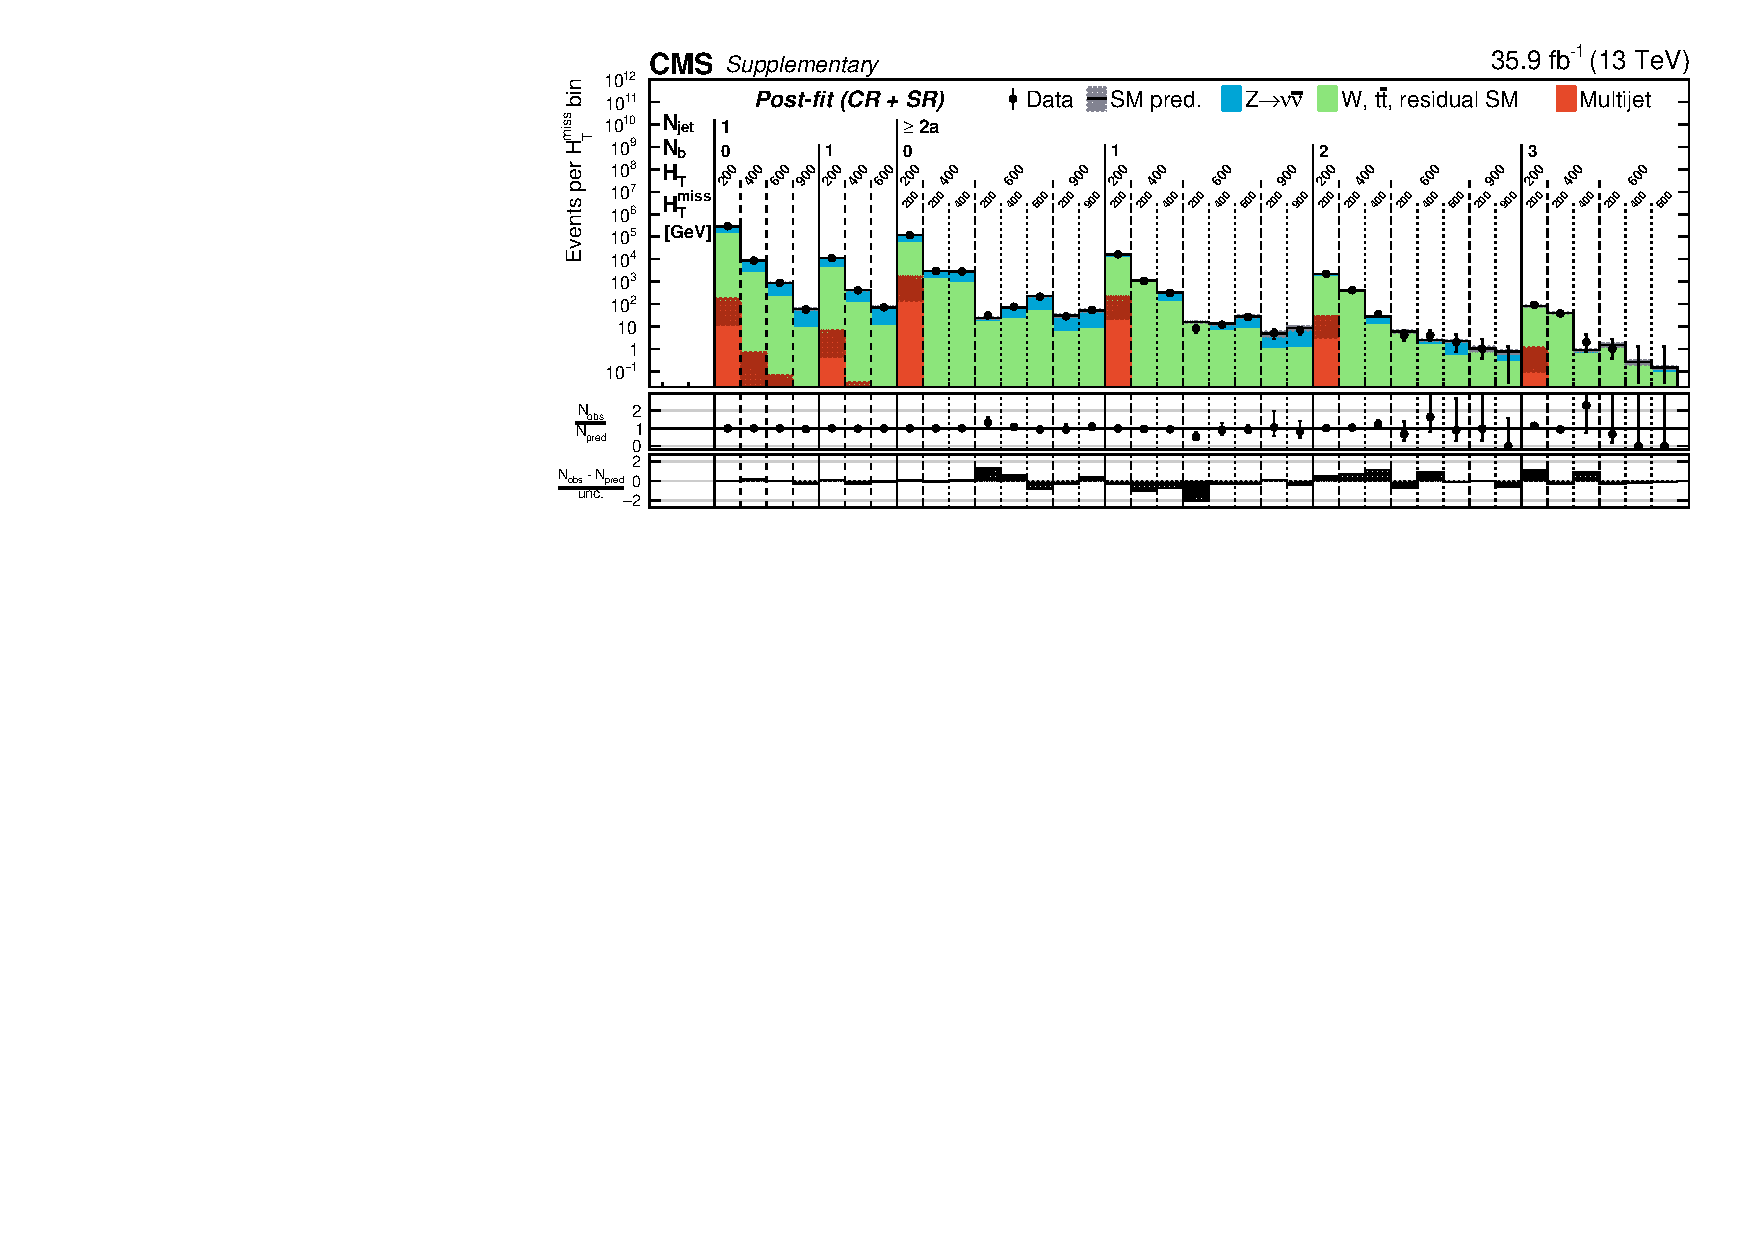
\includegraphics[width=0.99\textwidth, trim=0 0 0 0, 
clip=true]{figs/results/1jet_full.pdf}\\
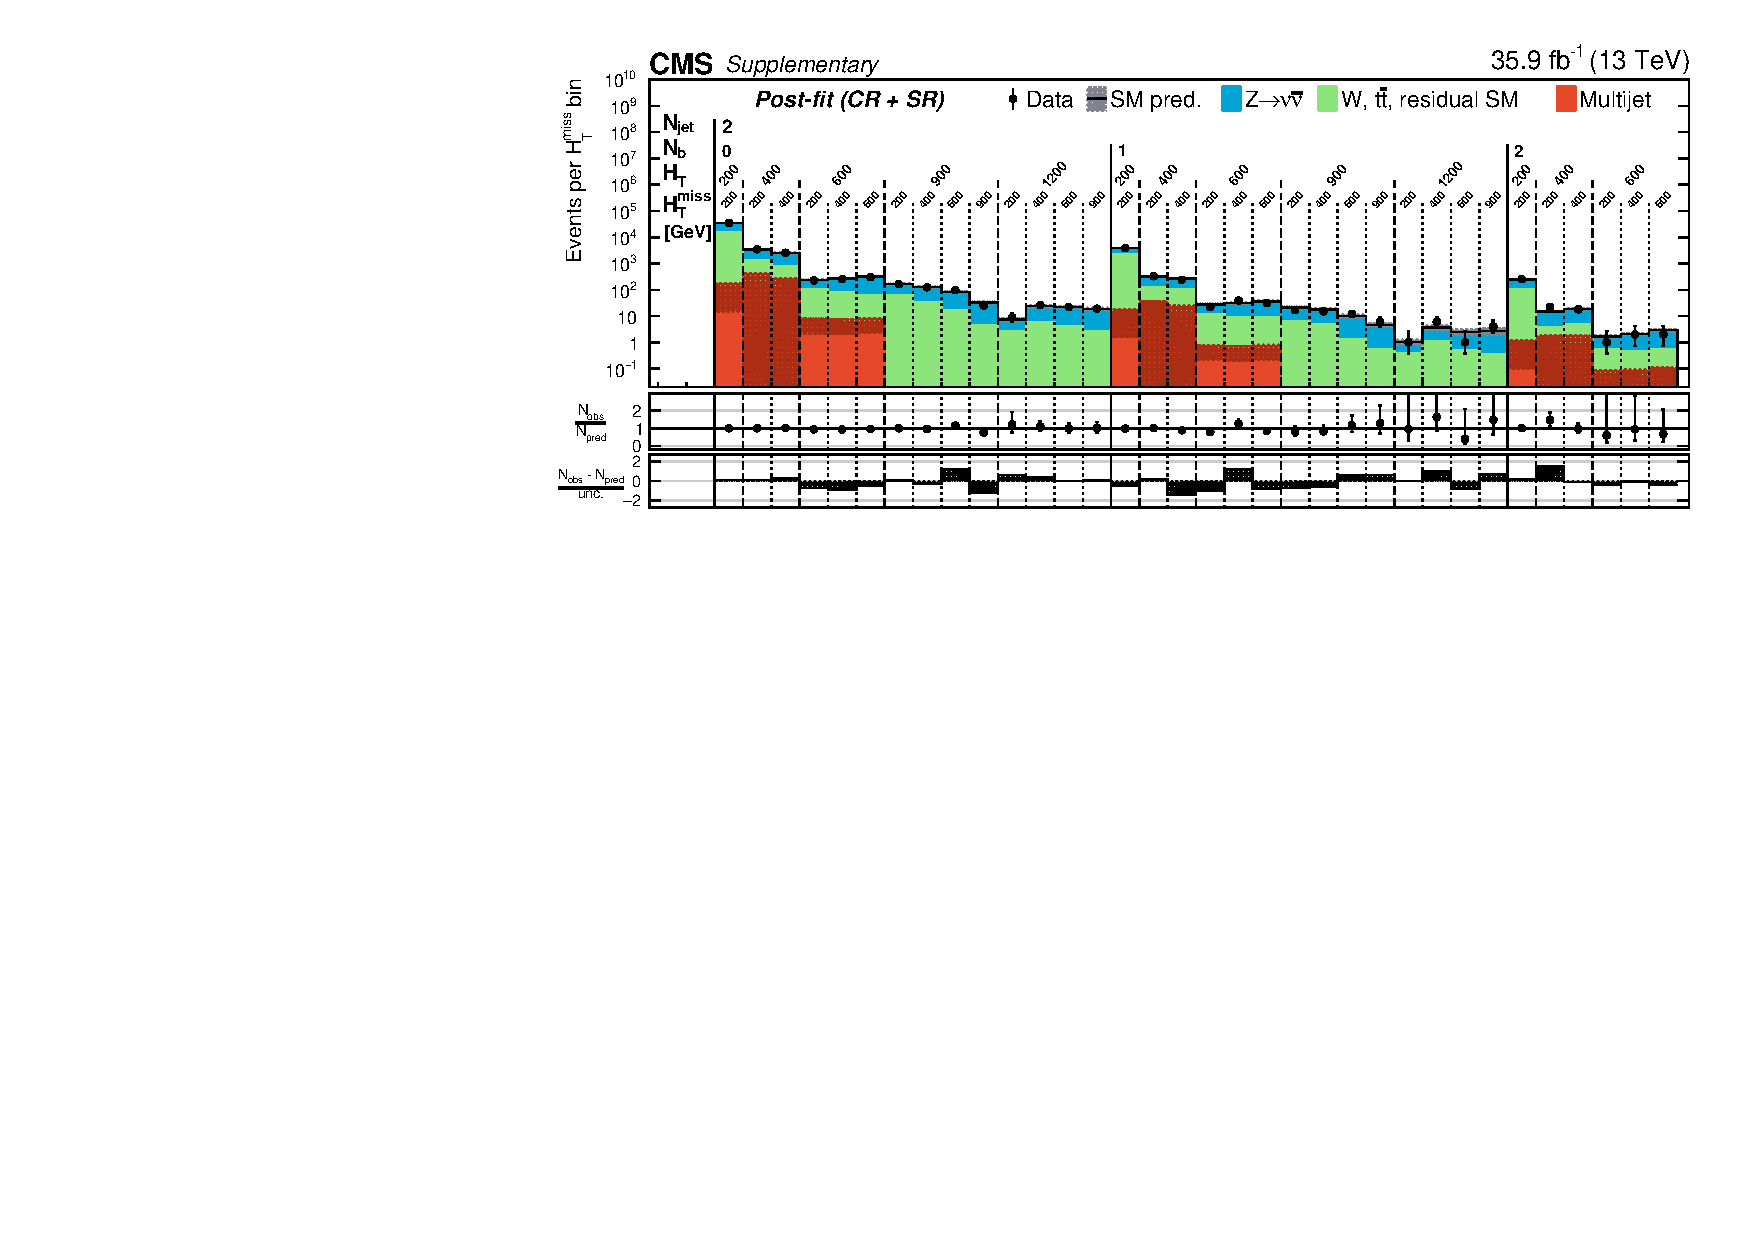
\includegraphics[width=0.99\textwidth, trim=0 0 0 0, 
clip=true]{figs/results/2jet_full.pdf}\\
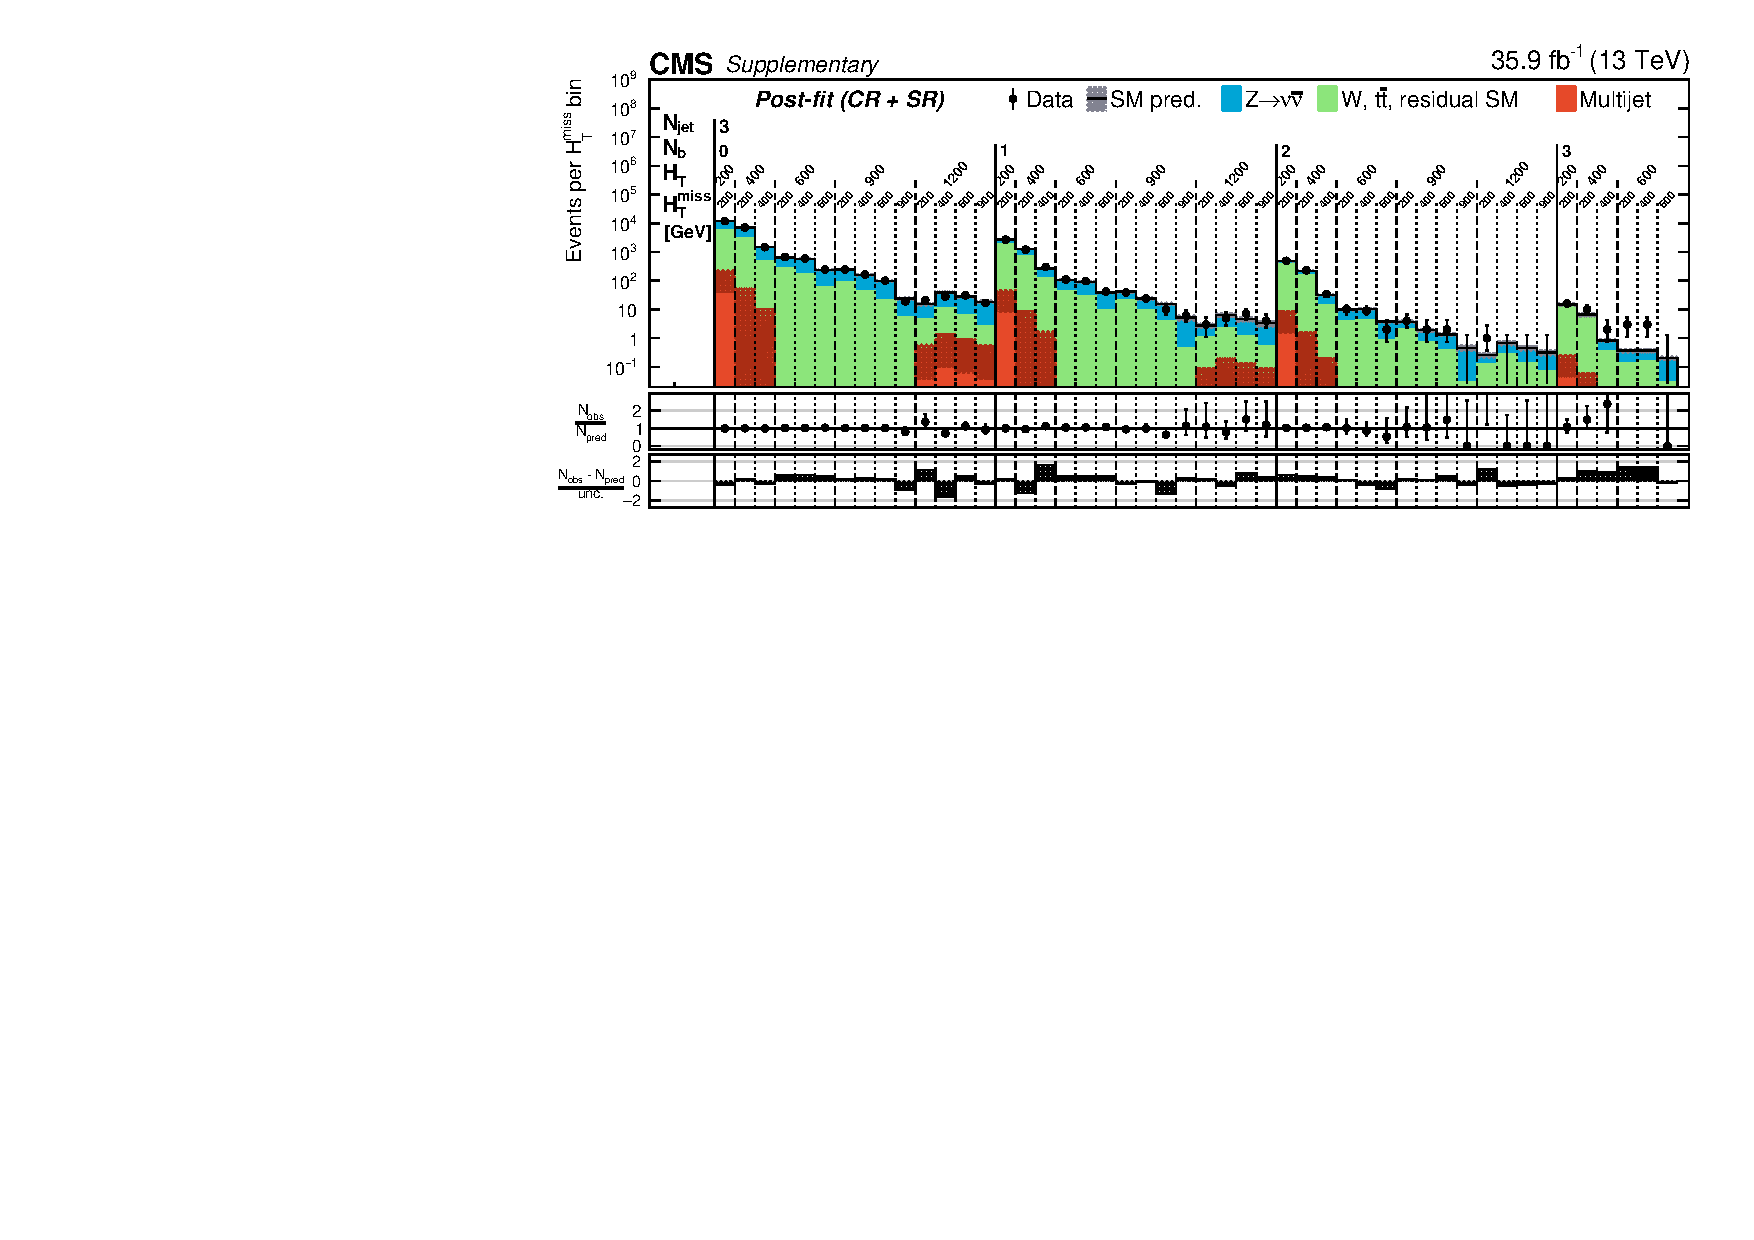
\includegraphics[width=0.99\textwidth, trim=0 0 0 0, 
clip=true]{figs/results/3jet_full.pdf}\\
\caption{Number of events observed (solid markers) and expected number of Z, 
\ttw and QCD background events (histograms, with shaded bands representing the 
statistical and systematic uncertainties) in every \nb, \scalht and \mht bin of 
the jet categories $\njet = 1, \ge2a$ (top), $\njet=2$ (middle), and $\njet=3$ 
(bottom), as determined from the maximum likelihood fit to the signal and 
control regions. 
The centre panel of each sub-figure shows the ratios of the observed and 
expected counts, while the lower panel shows the corresponding z-score, as 
defined in the text.}
\label{fig:results1-fullfit}
\end{figure}

\begin{figure}[!p]
\centering
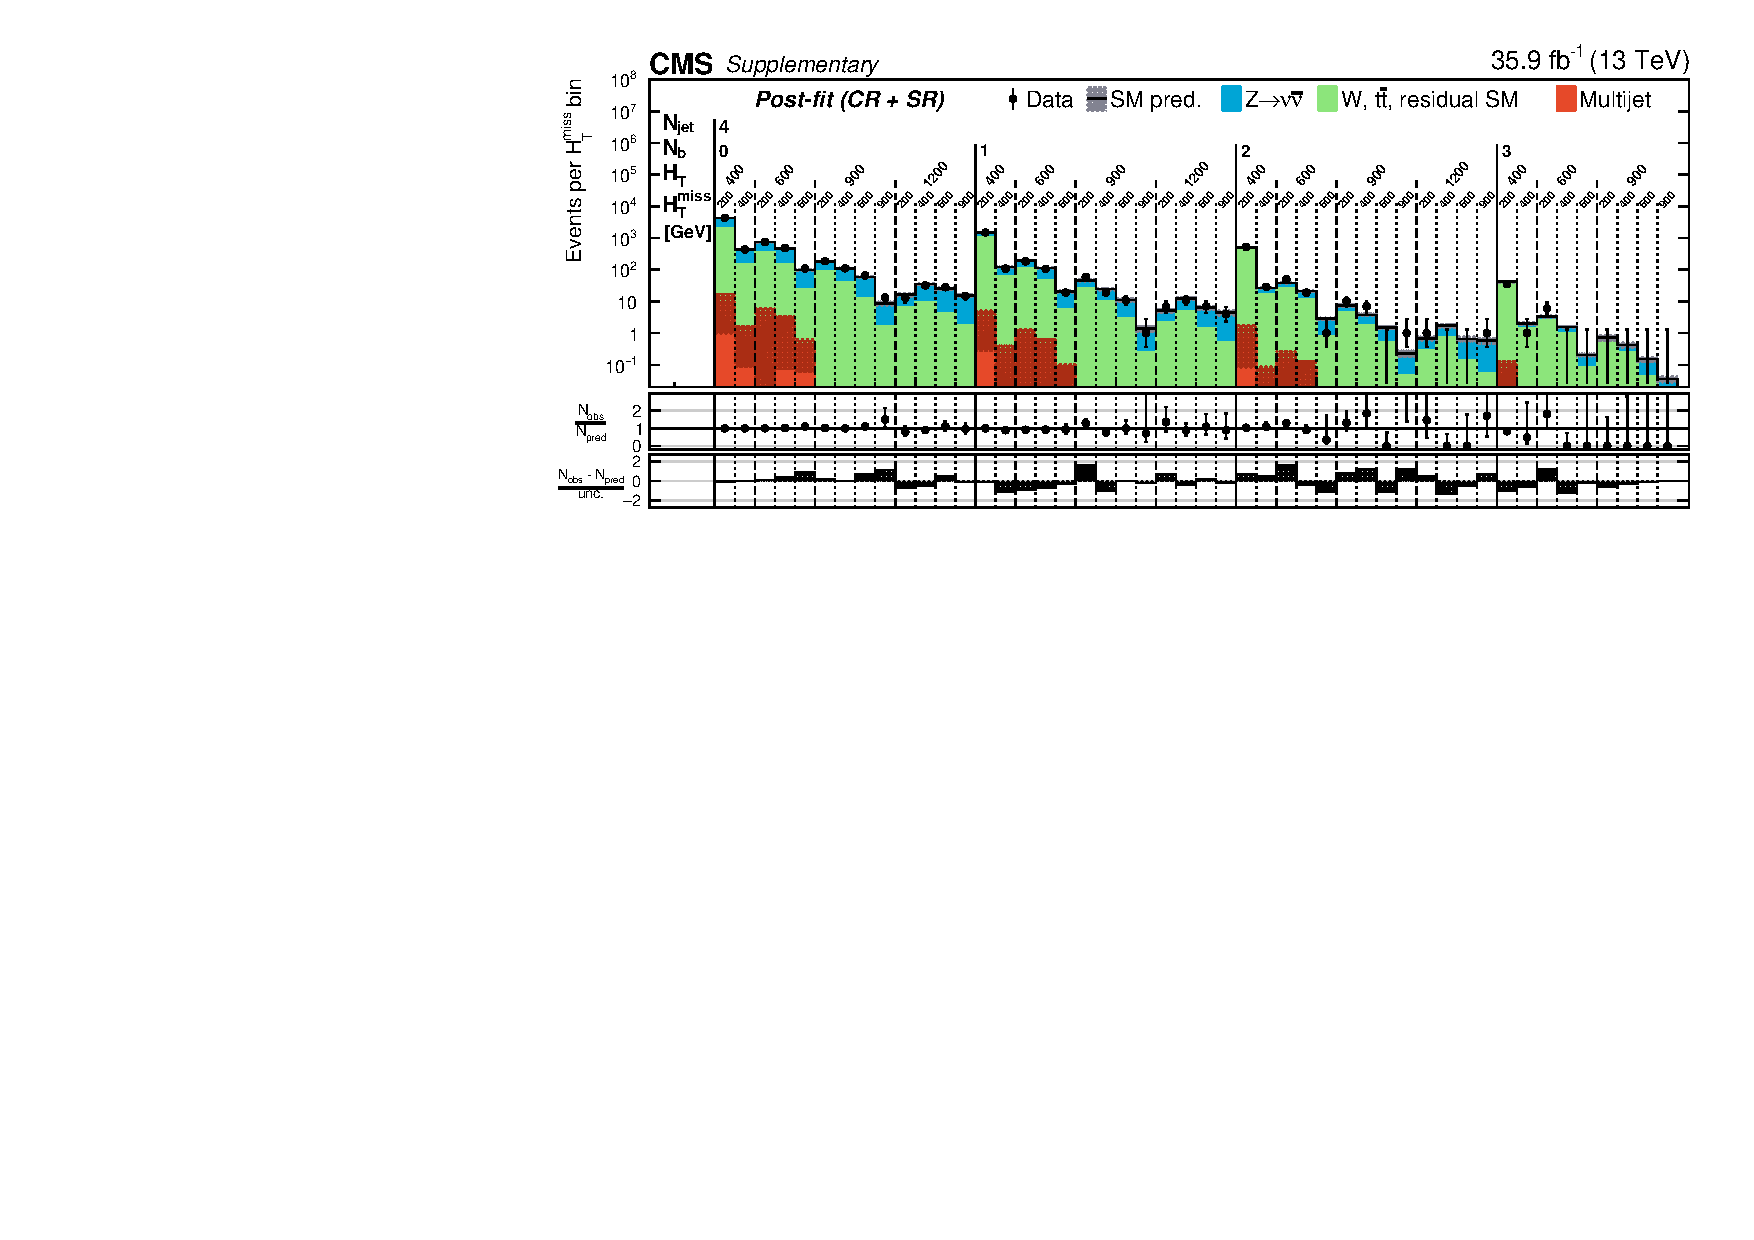
\includegraphics[width=0.99\textwidth, trim=0 0 0 0, 
clip=true]{figs/results/4jet_full.pdf}\\
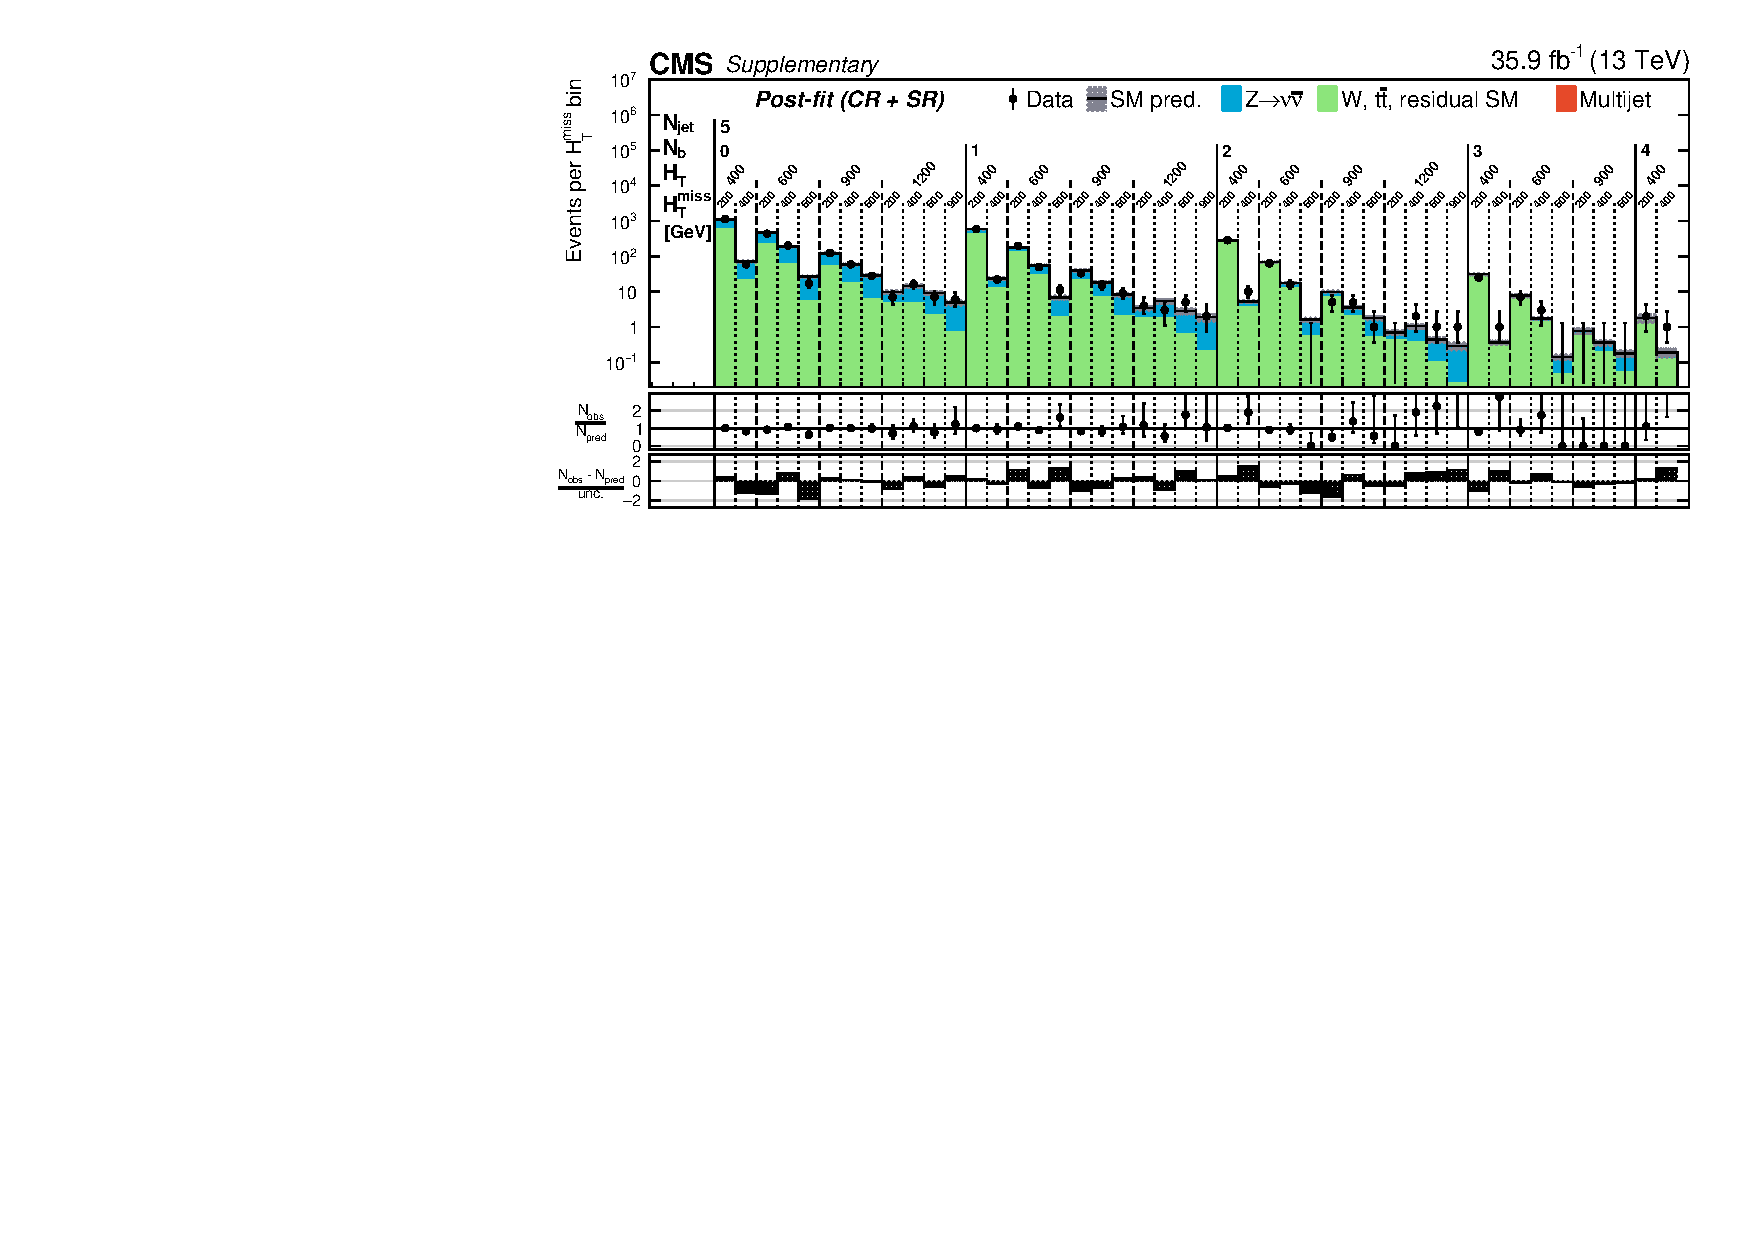
\includegraphics[width=0.99\textwidth, trim=0 0 0 0, 
clip=true]{figs/results/5jet_full.pdf}\\
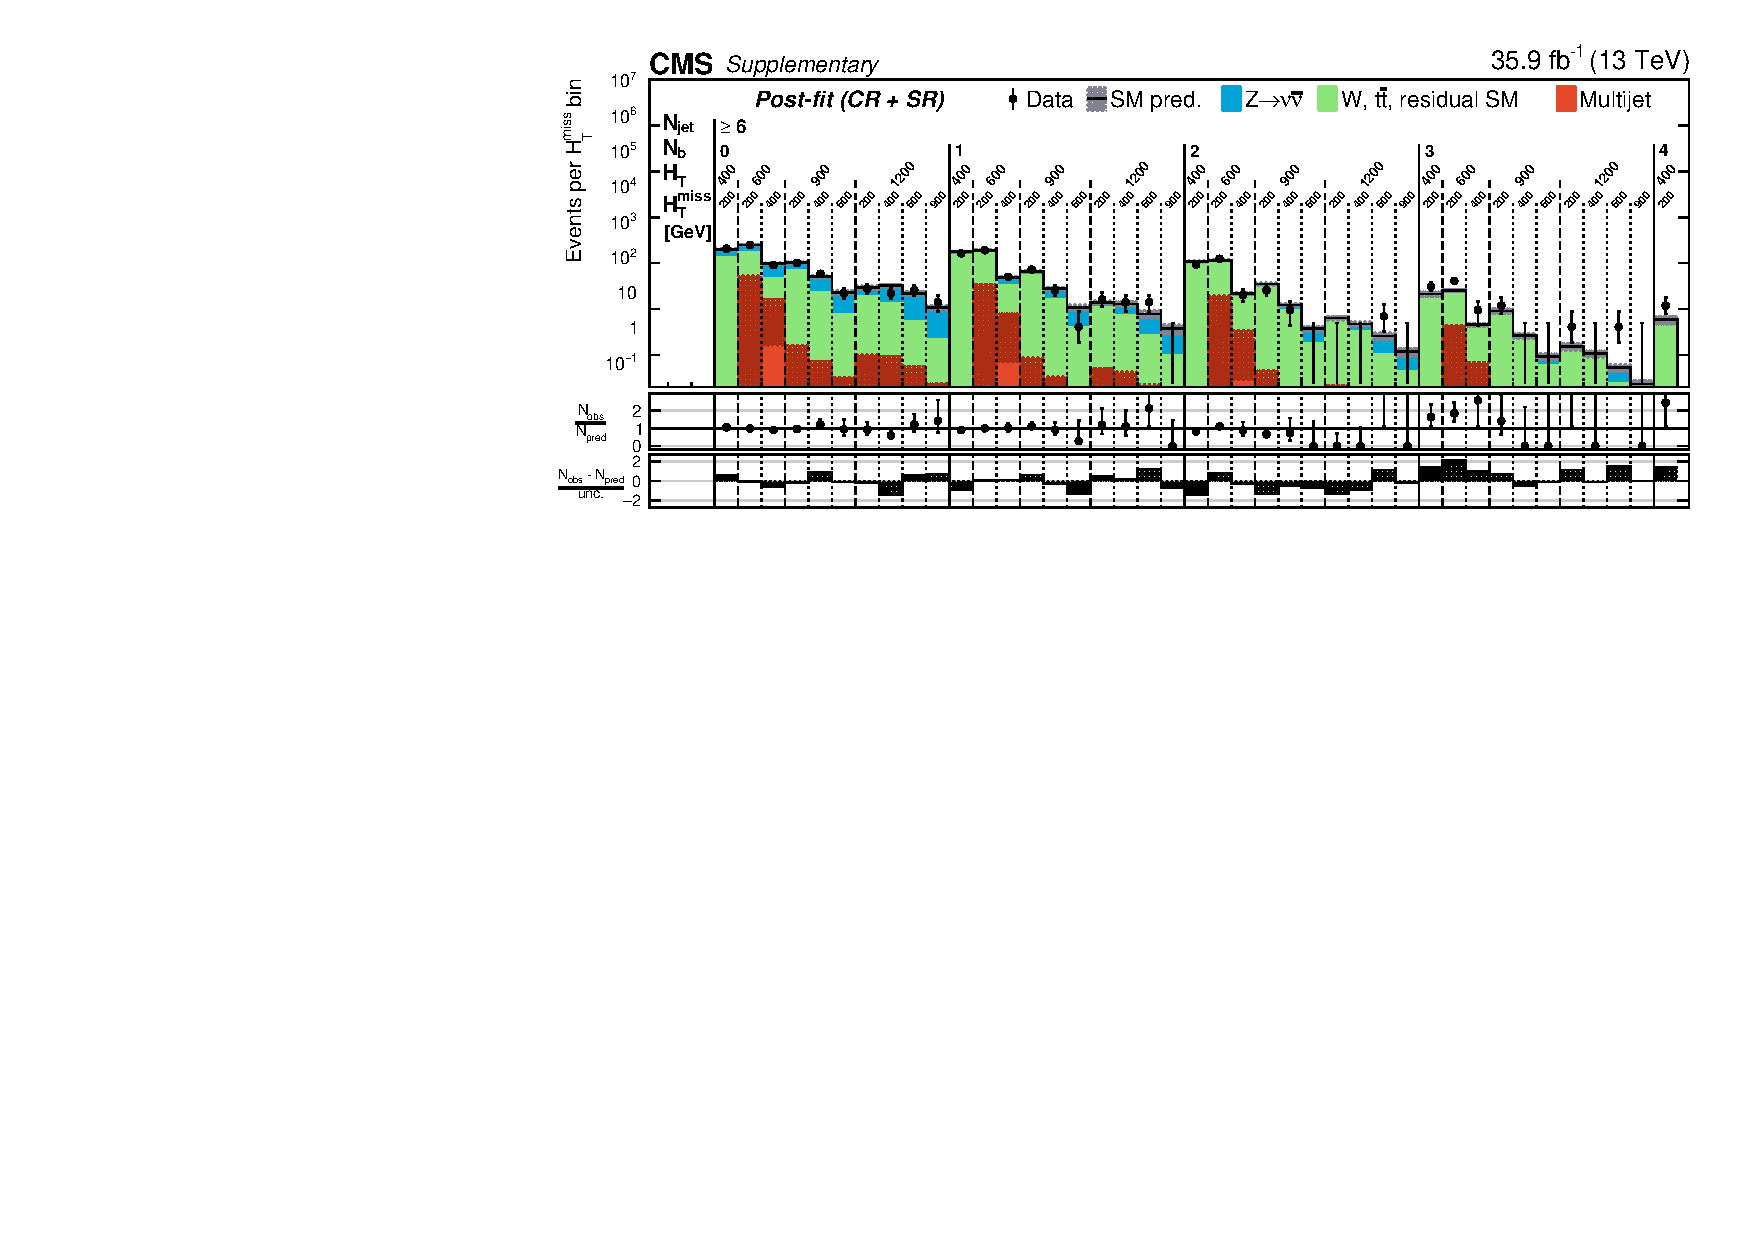
\includegraphics[width=0.99\textwidth, trim=0 0 0 0, 
clip=true]{figs/results/6jet_full.pdf}\\
\caption{Number of events observed (solid markers) and expected number of Z, 
\ttw and QCD background events (histograms, with shaded bands representing the 
statistical and systematic uncertainties) in every \nb, \scalht and \mht bin of 
the jet categories $\njet = 4$ (top), $\njet=5$ (middle), and $\njet\ge6$ 
(bottom), as determined from the background-only maximum likelihood fit to the 
signal and control regions. 
The centre panel of each sub-figure shows the ratios of the observed and 
expected counts, while the lower panel shows the corresponding z-score, as 
defined in the text.}
\label{fig:results2-fullfit}
\end{figure}

\clearpage
\section{Nuisance parameters}
\label{app:nuisances}
This appendix shows the best fit values (and their uncertainties) of the 
nuisance parameters that encode the systematic uncertainties on the background 
estimates under a likelihood fit to the signal and control regions for the 
background-only hypothesis, as discussed in Sec.~\ref{sec:results-results}.

%\begin{figure}[h!]
%	\centering
%	\caption{Rate parameters}
%	
%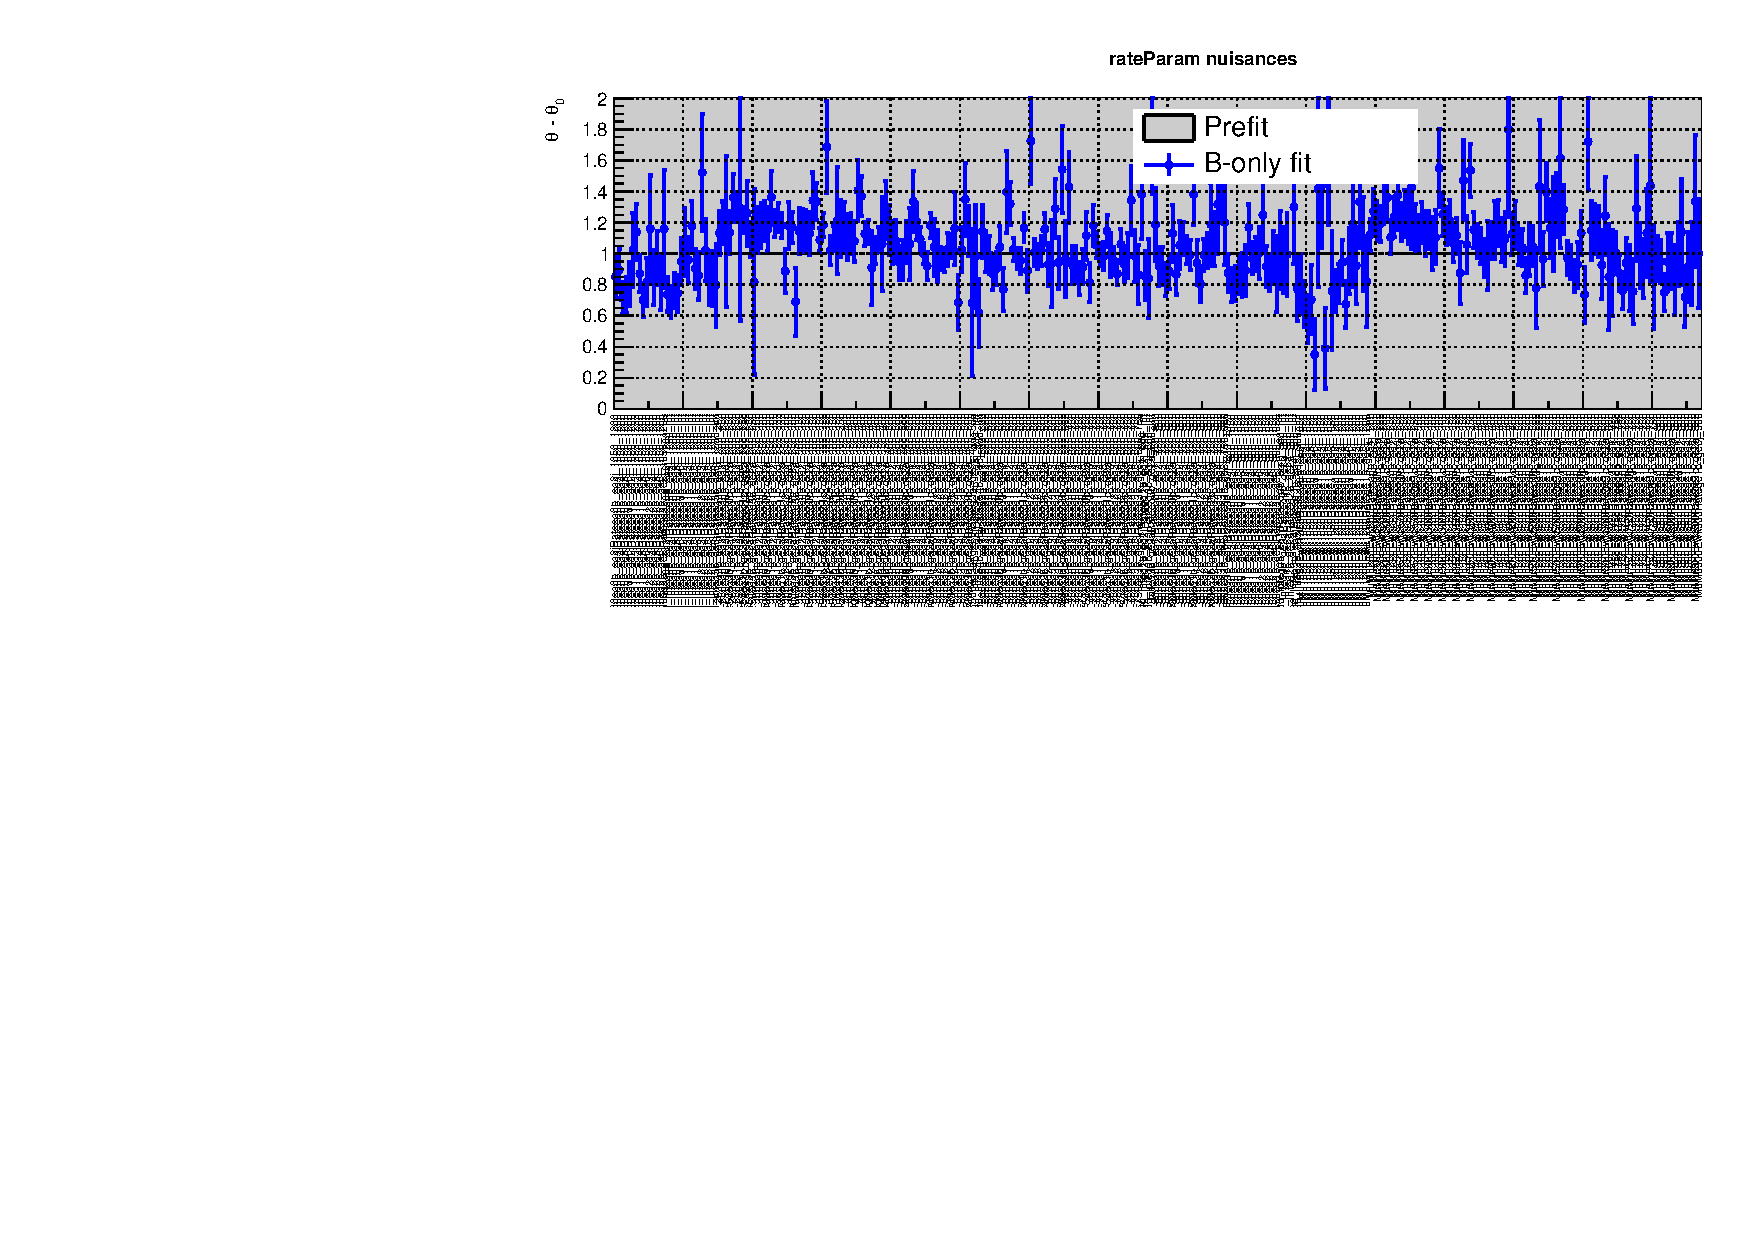
\includegraphics[width=1.\linewidth]{figures/results/36invfb_approval/postfit/nuis/Rates_nuisances}
%\end{figure}

\begin{figure}[h!]
	\centering
	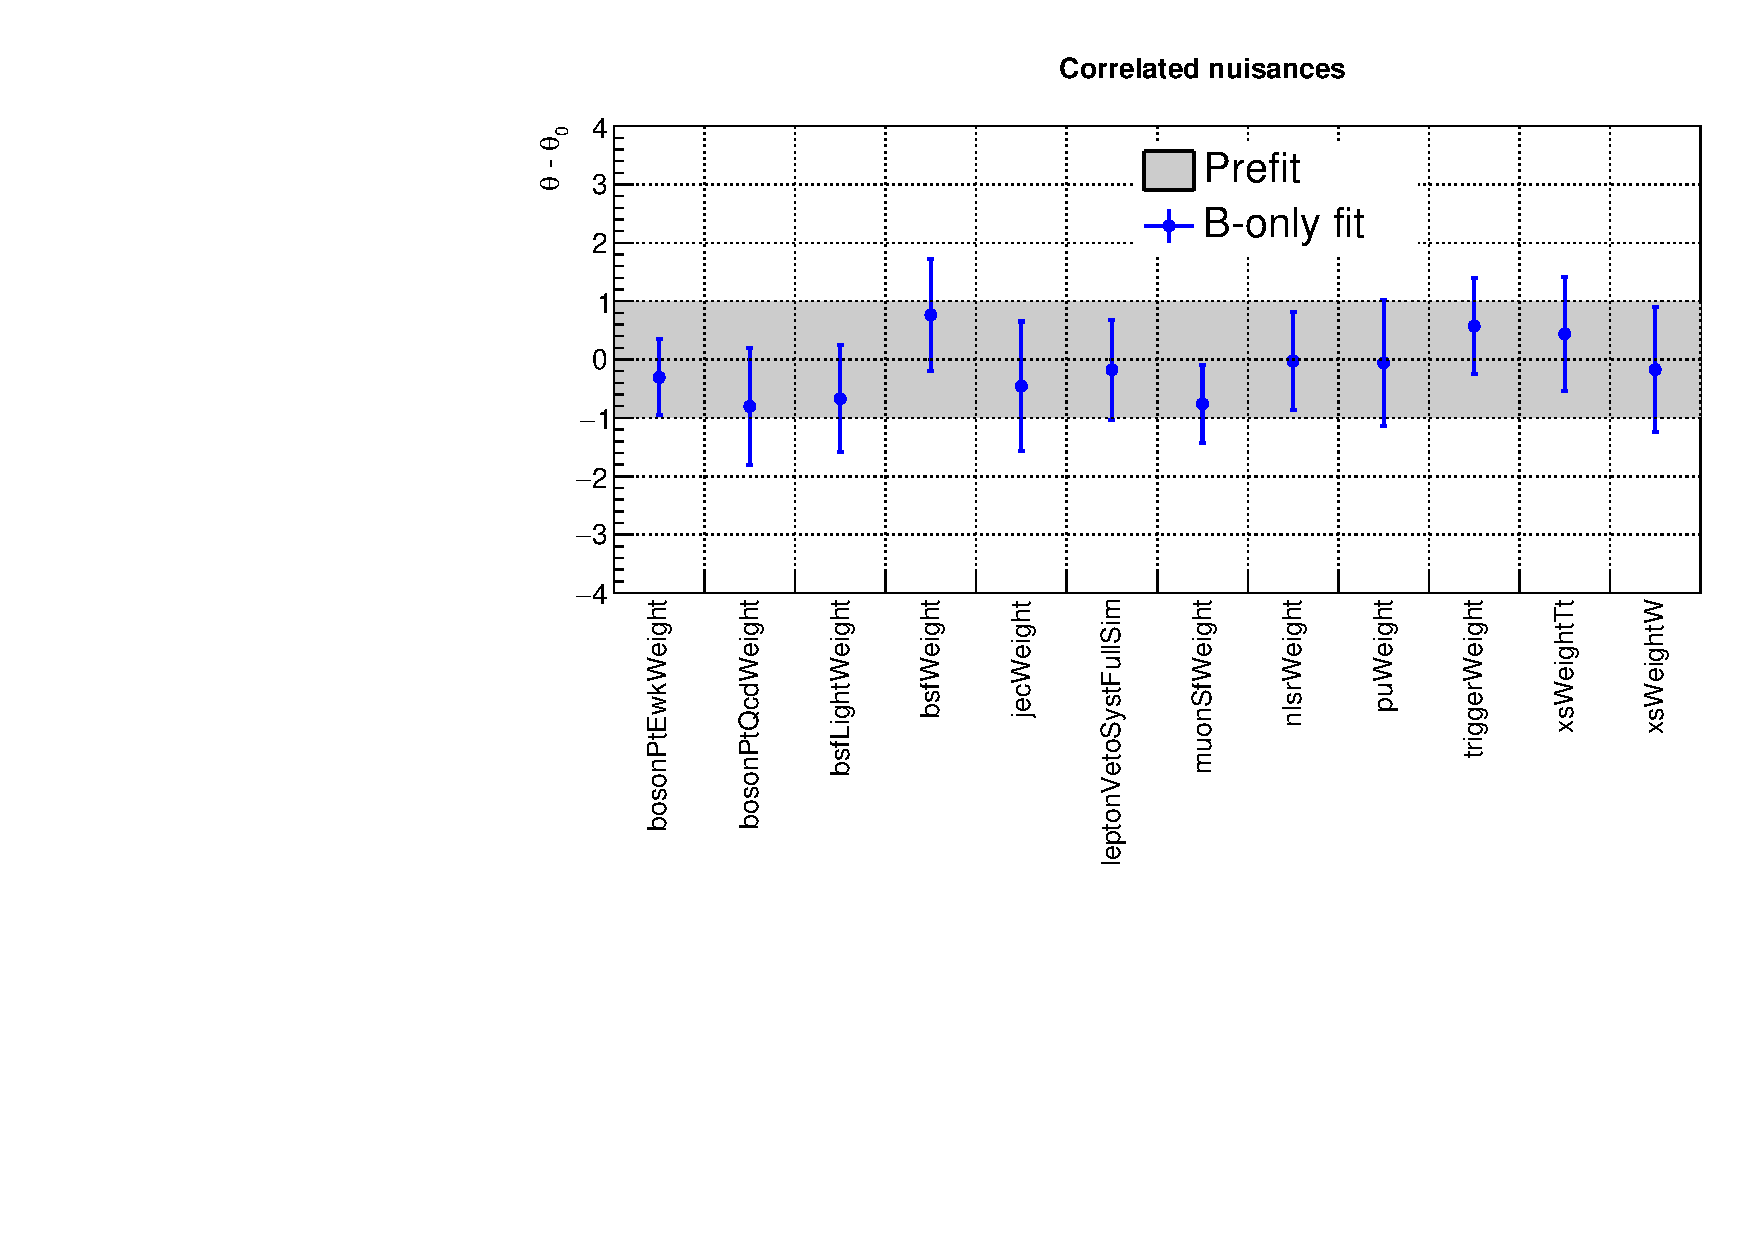
\includegraphics[width=1.\linewidth]{figs/results/nuis/Correlated_nuisances}
	\caption{Maximum likelihood values of the nuisance parameters related to 
	the systematic uncertainties derived from variations in the simulation 
	correction factors, as determined from the background-only fit to the 
	signal and control regions. From left to right: \pt dependent NLO QCD+EWK 
	corrections; b-tagging efficiency for light and heavy quarks; jet energy 
	scale; lepton identification, isolation and trigger; ISR jets; pileup; 
	signal region triggers; W and \ttbar cross sections.}
\end{figure}

%\clearpage
\begin{figure}[h!]
	\centering
	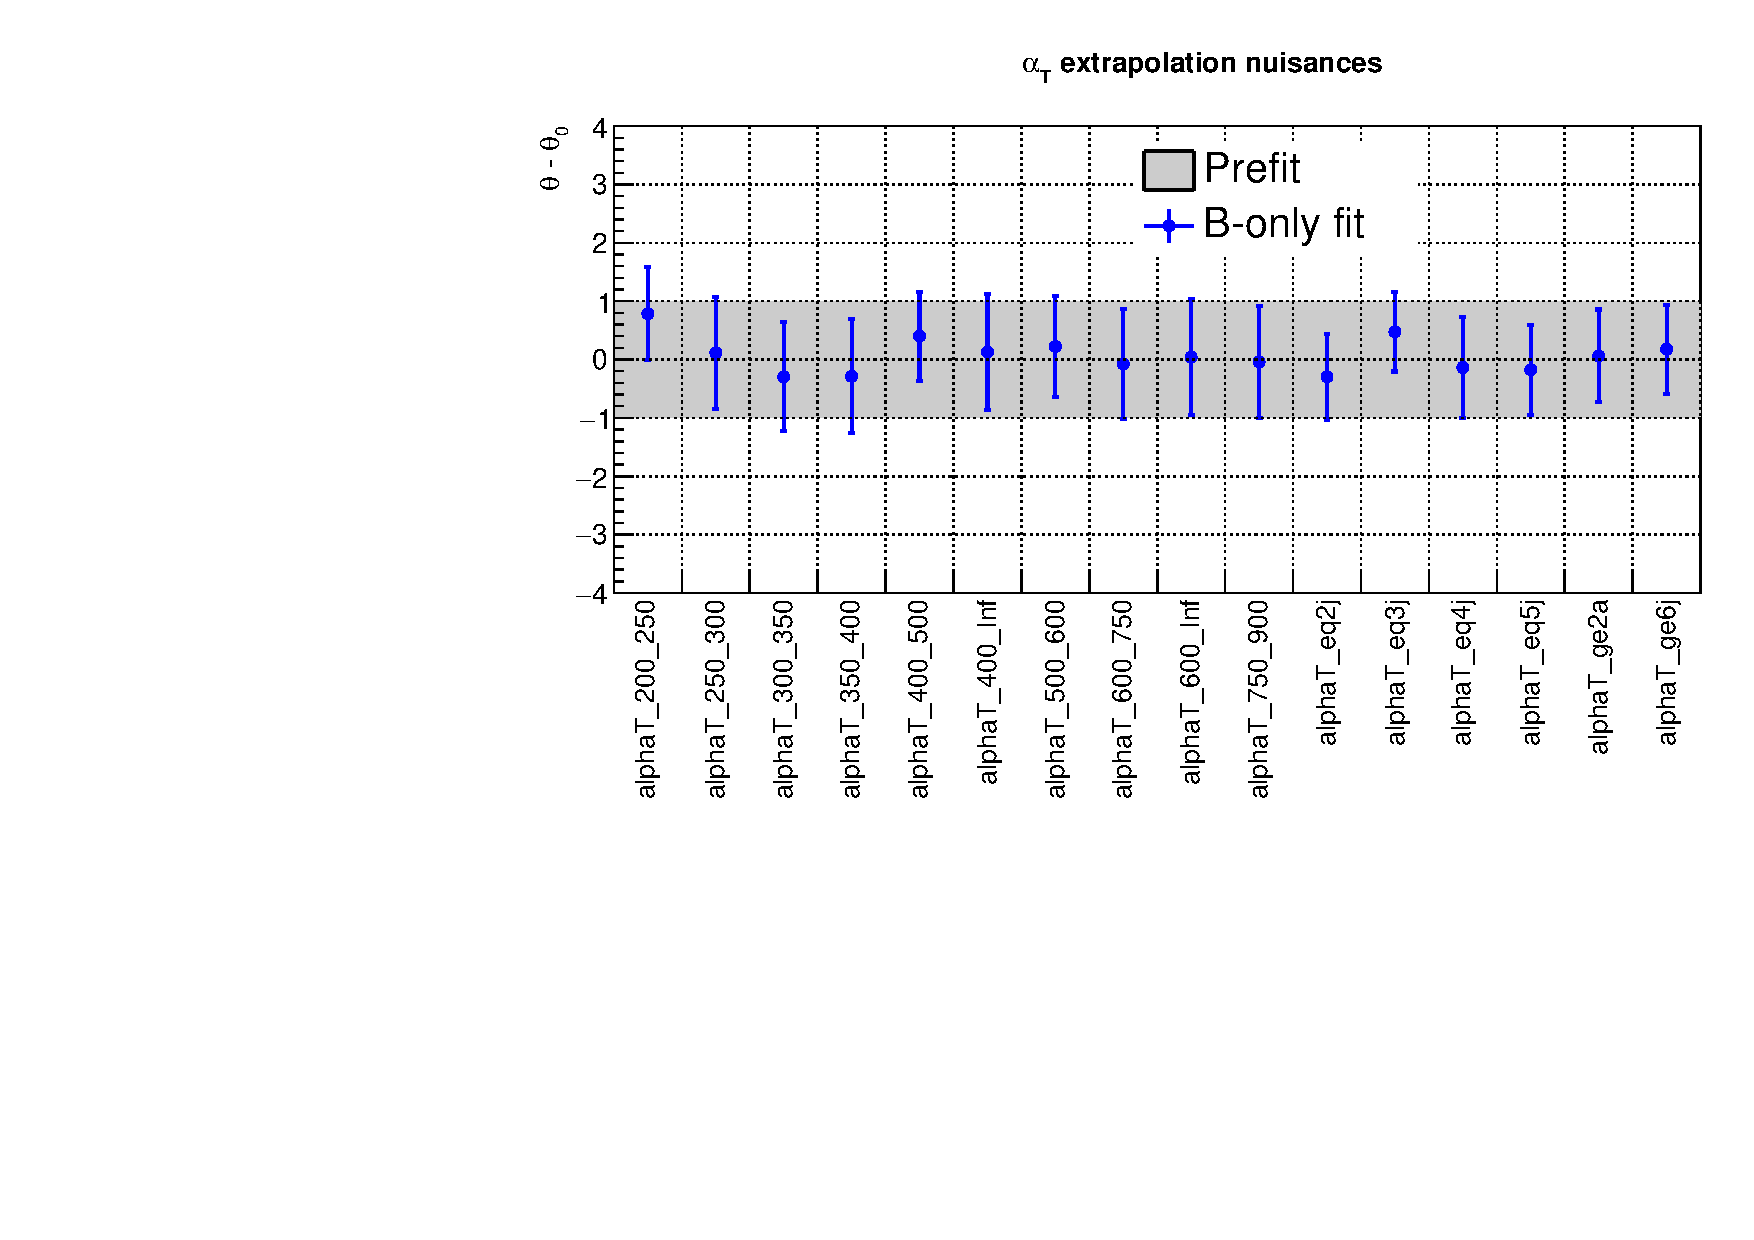
\includegraphics[width=0.8\linewidth]{figs/results/nuis/AlphaT_nuisances}
	\caption{Maximum likelihood values of the nuisance parameters related to 
	the systematic uncertainties derived from the \alphat closure tests, as 
	determined from the background-only fit to the signal and control regions.}
\end{figure}

\begin{figure}[h!]
	\centering
	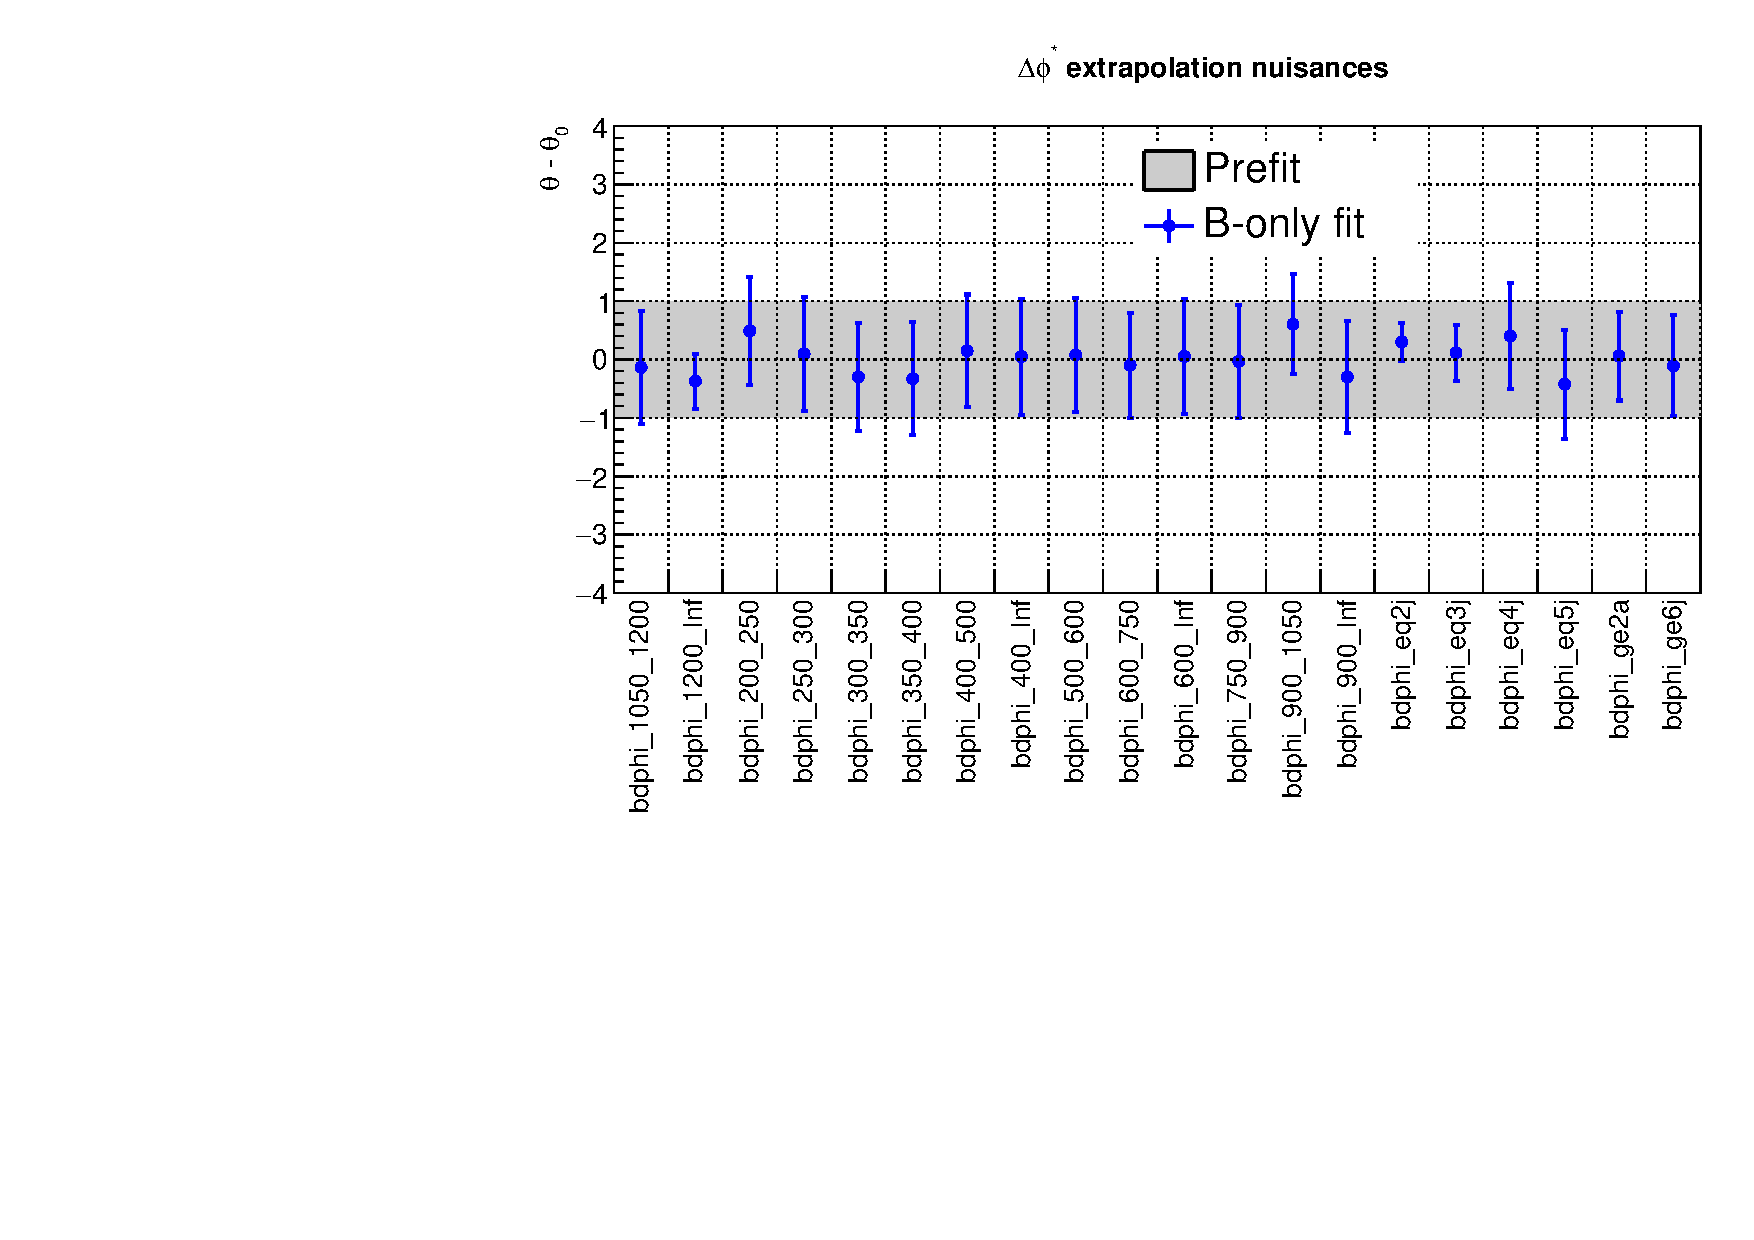
\includegraphics[width=0.8\linewidth]{figs/results/nuis/bDPhi_nuisances}
	\caption{Maximum likelihood values of the nuisance parameters related to 
	the systematic uncertainties derived from the \bdphi closure tests, as 
	determined from the background-only fit to the signal and control regions.}
\end{figure}

%\clearpage
%\begin{figure}[h!]
%	\centering
%	\caption{Systematic uncertainties in single isolated track veto modelling}
%	
%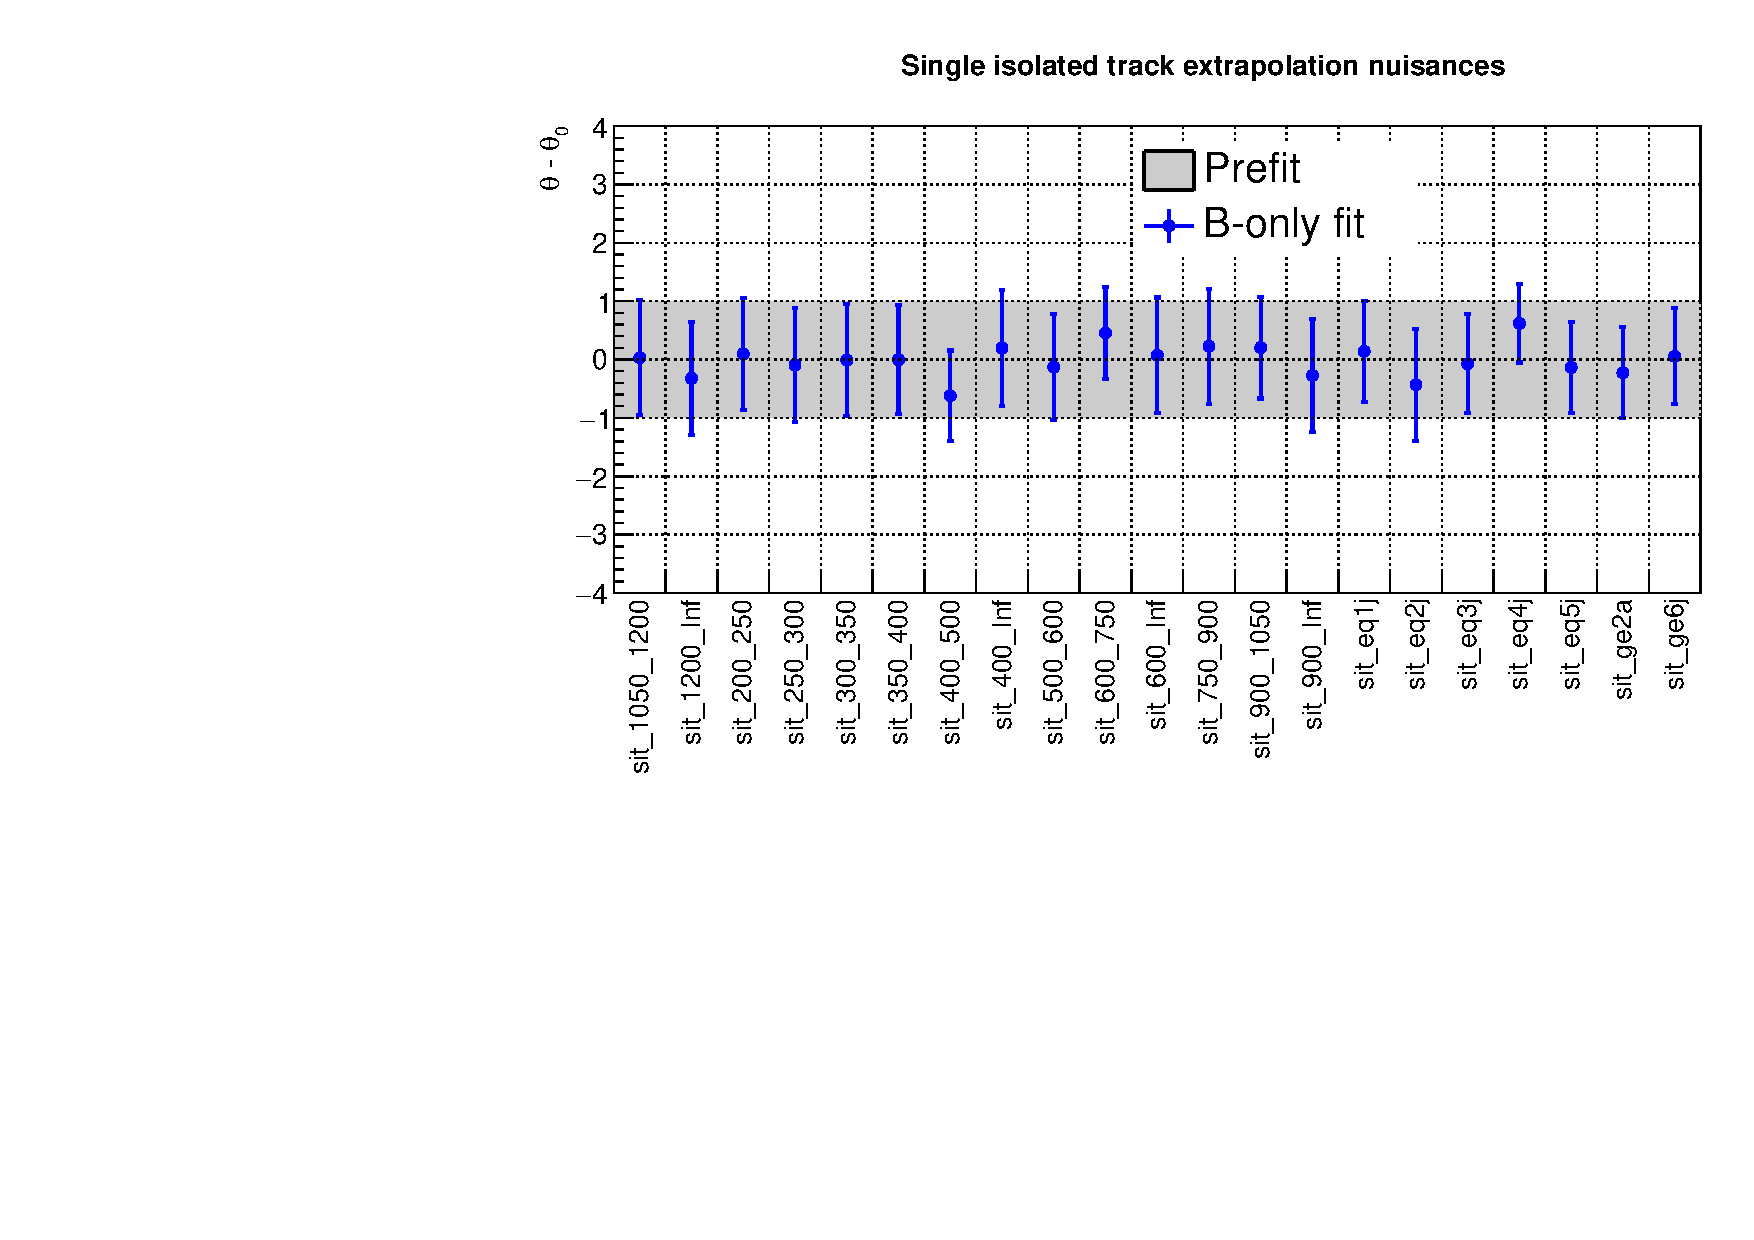
\includegraphics[width=0.8\linewidth]{figures/results/36invfb_approval/postfit/nuis/SIT_nuisances}
%\end{figure}

%\clearpage
\begin{figure}[h!]
	\centering
	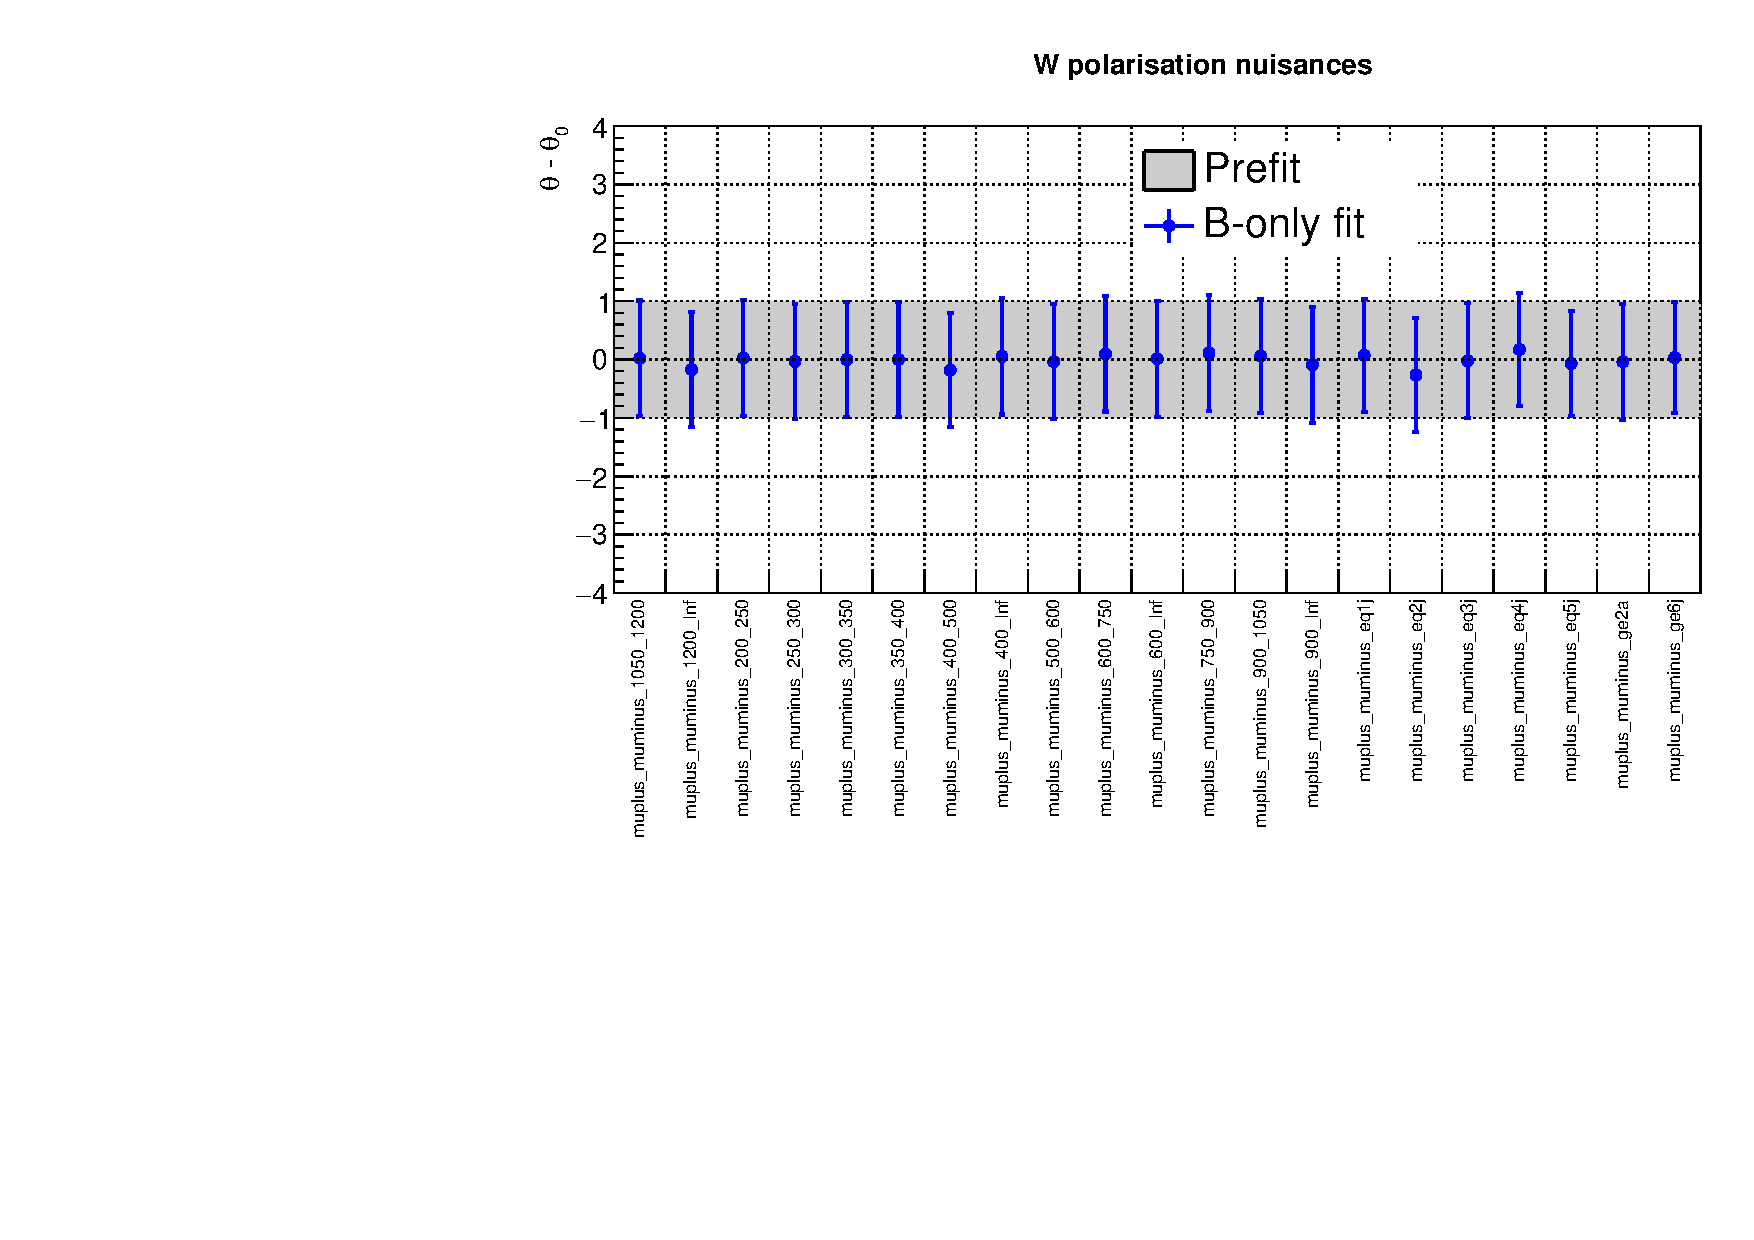
\includegraphics[width=0.8\linewidth]{figs/results/nuis/WPol_nuisances}
	\caption{Maximum likelihood values of the nuisance parameters related to 
	the systematic uncertainties derived from the W$^{+}$/W$^{-}$ closure 
	tests, as determined from the background-only fit to the signal and control 
	regions.}
\end{figure}

%\clearpage
%\begin{figure}[h!]
%	\centering
%	\caption{``MC stat.'' uncertainties for lost lepton background.}
%	
%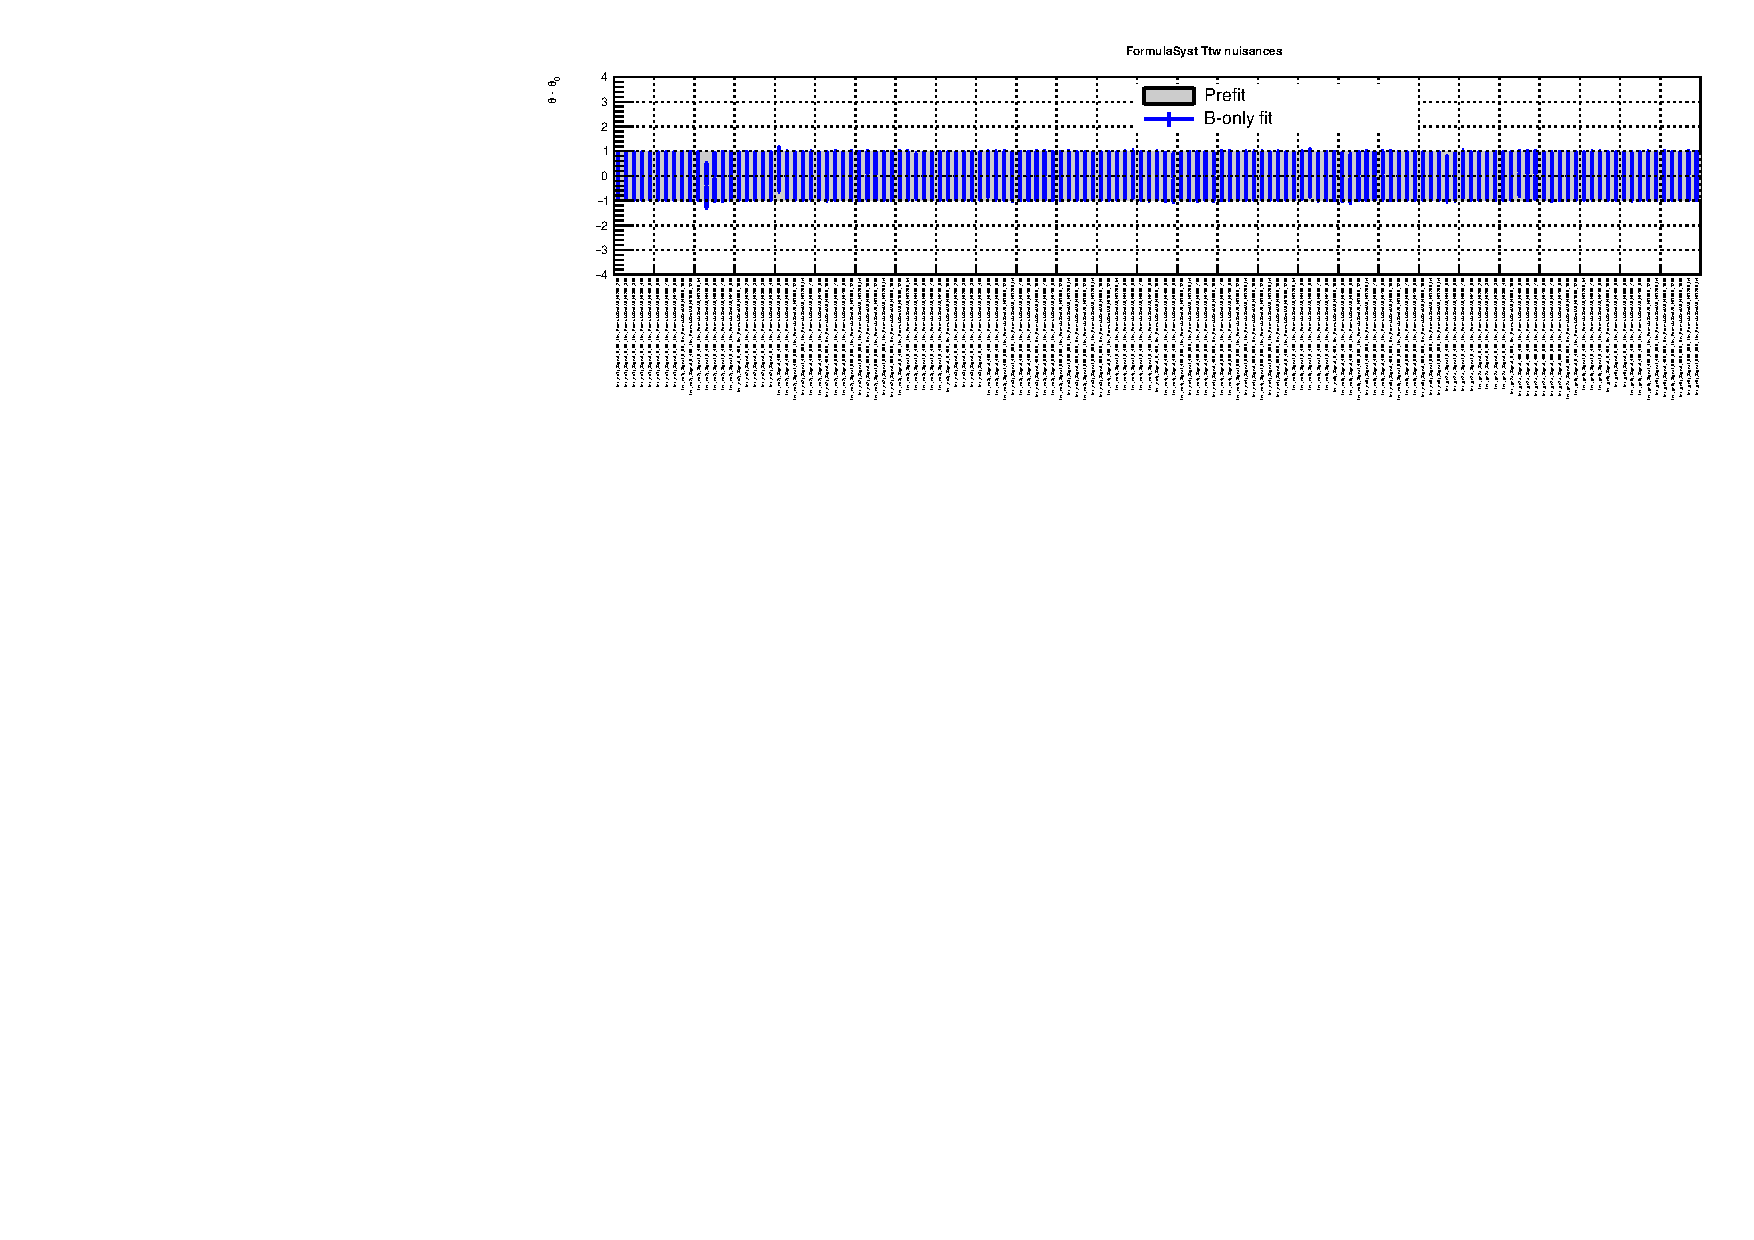
\includegraphics[width=1.\linewidth]{figures/results/36invfb_approval/postfit/nuis/FormulaSystTtw_nuisances}
%\end{figure}

%\begin{figure}[h!]
%	\centering
%	\caption{``MC stat.'' uncertainties for \znunuj background.}
%	
%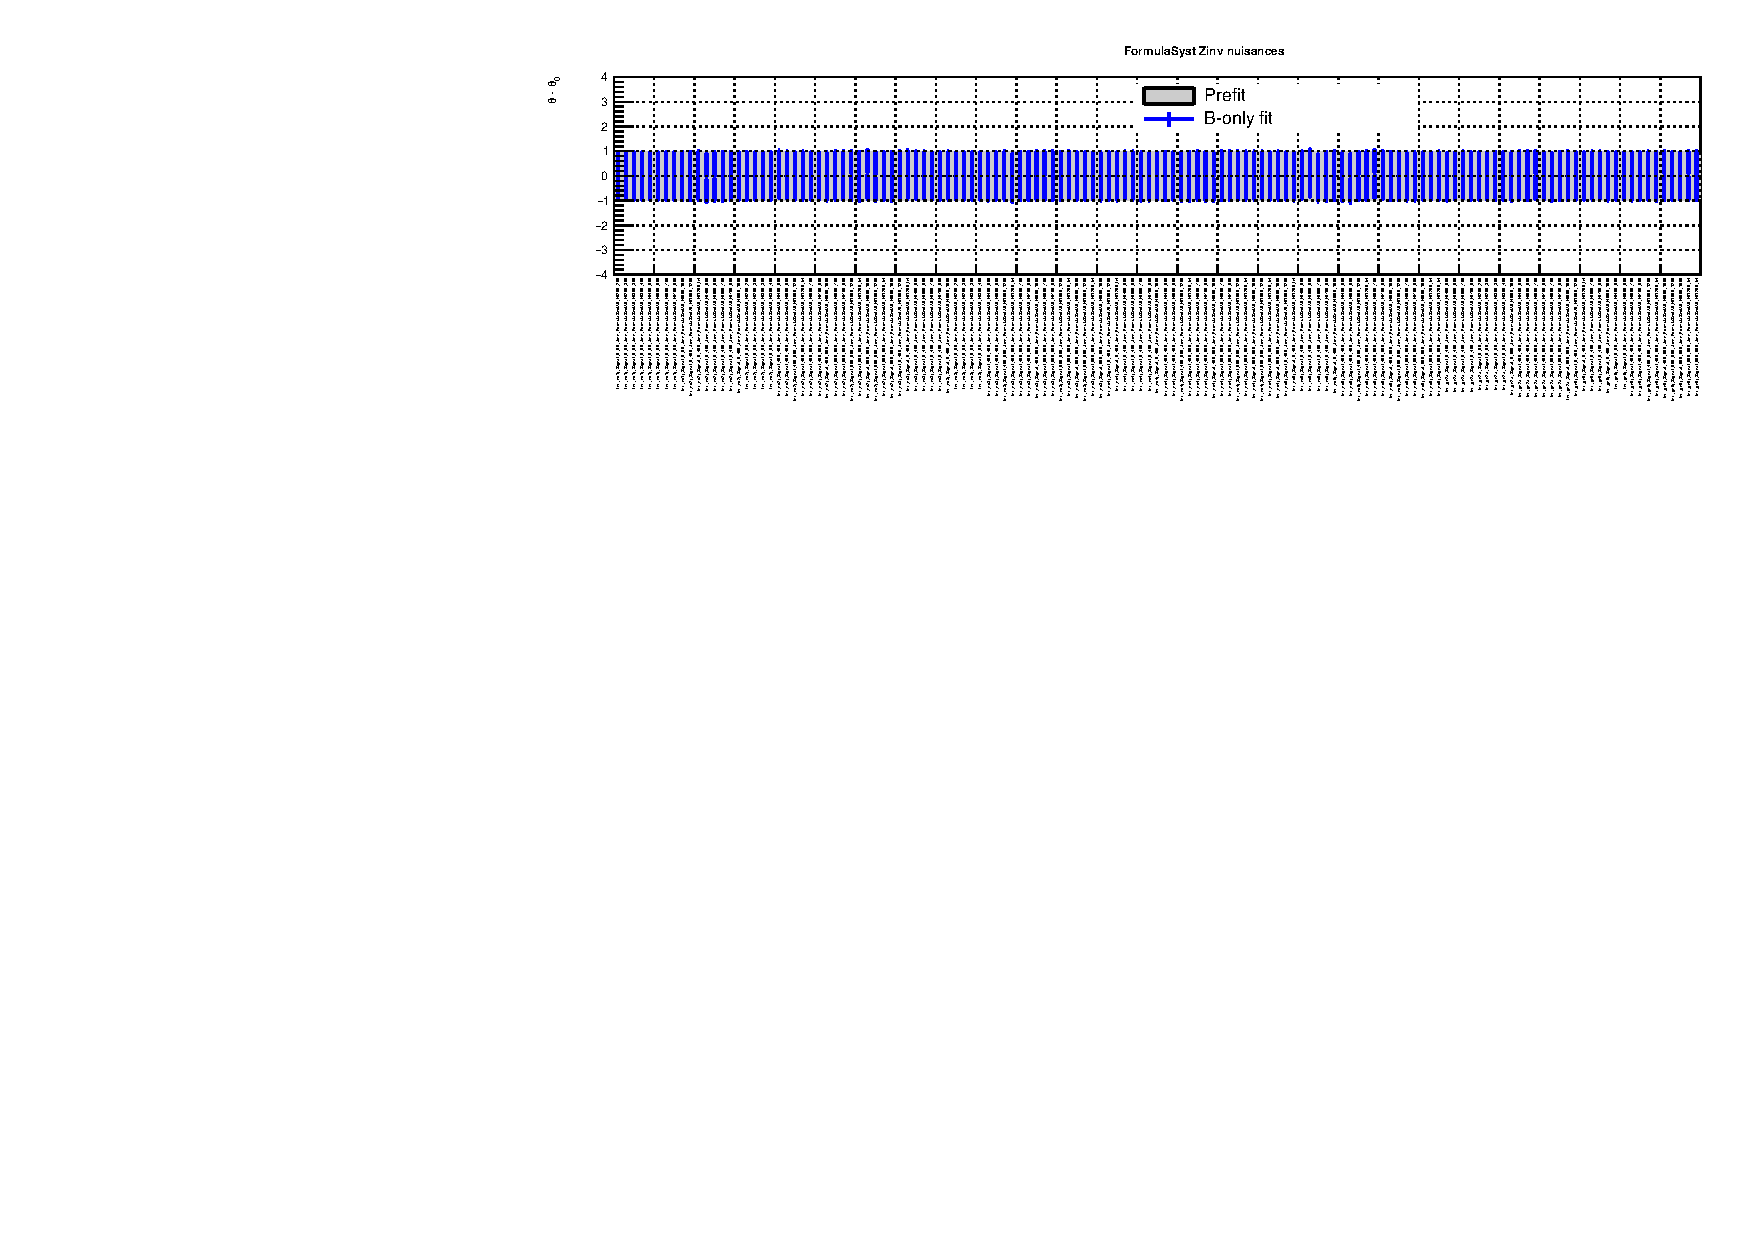
\includegraphics[width=1.\linewidth]{figures/results/36invfb_approval/postfit/nuis/FormulaSystZinv_nuisances}
%\end{figure}

\clearpage
\begin{figure}[h!]
	\centering
	\includegraphics[width=1.\linewidth]{figs/results/nuis/TemplateTtw_ht_nuisances}
	\caption{Maximum likelihood values of the nuisance parameters related to 
	the \scalht-dependent systematic uncertainties on the \mht shape of the 
	\ttw processes, as determined from the background-only fit to the signal 
	and control regions.}
\end{figure}

\begin{figure}[h!]
	\centering
	\includegraphics[width=1.\linewidth]{figs/results/nuis/TemplateTtw_njet_nuisances}
	\caption{Maximum likelihood values of the nuisance parameters related to 
	the \njet-dependent systematic uncertainties on the \mht shape of the \ttw 
	processes, as determined from the background-only fit to the signal and 
	control regions.}
\end{figure}

%\clearpage
\begin{figure}[h!]
	\centering
	\includegraphics[width=1.\linewidth]{figs/results/nuis/TemplateZinv_ht_nuisances}
	\caption{Maximum likelihood values of the nuisance parameters related to 
	the \scalht-dependent systematic uncertainties on the \mht shape of the 
	\znnj process, as determined from the background-only fit to the signal and 
	control regions.}
\end{figure}

\begin{figure}[h!]
	\centering
	\includegraphics[width=1.\linewidth]{figs/results/nuis/TemplateZinv_njet_nuisances}
	\caption{Maximum likelihood values of the nuisance parameters related to 
	the \njet-dependent systematic uncertainties on the \mht shape of the \znnj 
	process, as determined from the background-only fit to the signal and 
	control regions.}
\end{figure}

%\clearpage
\begin{figure}[h!]
	\centering
	\includegraphics[width=1.\linewidth]{figs/results/nuis/qcd_nuisances}
	\caption{Maximum likelihood values of the nuisance parameters related to 
	the systematic uncertainties on the QCD estimation, as determined from the 
	background-only fit to the signal and control regions.}
\end{figure}


%\chapter{Systematics}
%\label{app:systs}
%Hi.